\documentclass[%
 reprint,
%superscriptaddress,
%groupedaddress,
%unsortedaddress,
%runinaddress,
%frontmatterverbose, 
%preprint,
%showpacs,preprintnumbers,
nofootinbib,
nobibnotes,
%bibnotes,
 amsmath,amssymb,
% aps,
%pra,
%prb,
%rmp,
%prstab,
%prstper,
%floatfix,
]{revtex4-1}
%\documentclass{article}
\usepackage{geometry}                % See geometry.pdf to learn the layout options. There are lots.
%\geometry{letterpaper}                   % ... or a4paper or a5paper or ...
%\geometry{landscape}                % Activate for for rotated page geometry
%\usepackage[parfill]{parIEEEabrvskip}    % Activate to begin paragraphs with an empty line rather than an indent
\usepackage{graphicx}
\usepackage{caption}
\usepackage{subcaption}
\usepackage{dcolumn}% Align table columns on decimal point
\usepackage{bm}% bold math
%\usepackage{amssymb}
%\usepackage{amsmath}
\usepackage{epstopdf}
\usepackage{amsthm}

\usepackage{pifont} % check and x marks
\usepackage{color}

\newcommand{\cmark}{\ding{51}}
\newcommand{\xmark}{\ding{55}}

\newcommand{\gcc}{{\tt 403.gcc}~}
\newcommand{\svd}{{\tt dgesdd}~}
\newcommand{\svdone}{{\tt dgesdd}$_1$~}
\newcommand{\svdtwo}{{\tt dgesdd$_2$}~}
\newcommand{\svdthree}{{\tt dgesdd$_3$}~}
\newcommand{\svdfour}{{\tt dgesdd$_4$}~}
\newcommand{\svdfive}{{\tt dgesdd$_5$}~}
\newcommand{\svdsix}{{\tt dgesdd$_6$}~}
\newcommand{\naive}{na\"ive}
\newcommand{\row}{{\tt row\_major}~}
\newcommand{\col}{{\tt col\_major}~}
%\newcommand{\color{red}}{{\color[rgb]{1,0,0}}}

%\parskip=3pt



%\usepackage{authblk}
%\DeclareGraphicsRule{.tif}{png}{.png}{`convert #1 `dirname #1`/`basename #1 .tif`.png}

\newtheorem*{mydef}{Definition}





%Version 1
%\author{
%  \IEEEauthorblockN{Joshua Garland}
%  \IEEEauthorblockA{Dept. of Computer Science\\
%    University of Colorado at Boulder\\
%    Colorado, USA\\
%    Email: joshua.garland@colorado.edu}
%  \and
%  \IEEEauthorblockN{Ryan G.~James}
%  \IEEEauthorblockA{Complexity Sciences Center \& Dept. of Physics\\
%    University of California at Davis\\
%    California, USA\\
%    Email: rgjames@ucdavis.edu}
%    \and
%      \IEEEauthorblockN{Elizabeth Bradley}
%         \IEEEauthorblockA{Santa Fe Institute \\
%    New Mexico, USA\\
%    }
%  \IEEEauthorblockA{Dept. of Computer Science\\
%    University of Colorado at Boulder\\
%    Colorado, USA\\
%    Email: lizb@colorado.edu}
%  }



 %\author{
 %  \IEEEauthorblockN{
 %    Joshua Garland\IEEEauthorrefmark{1},
 %    Ryan G.~James\IEEEauthorrefmark{1} and
 %    Elizabeth Bradley\IEEEauthorrefmark{1}\IEEEauthorrefmark{2}}
 %  \IEEEauthorblockA{
 %    \IEEEauthorrefmark{1}Dept. of Computer Science
 %    University of Colorado, Boulder, Colorado 80309-0430 USA\\
 %    Email: joshua.garland@colorado.edu, ryan.james@colorado.edu}
 %  \IEEEauthorblockA{
 %    \IEEEauthorrefmark{2}Santa Fe Institute, 1399 Hyde Park Road, Santa Fe, New Mexico 87501  USA\\
 %    Email: lizb@colorado.edu}
 %  % \IEEEauthorblockA{
 %  %   \IEEEauthorrefmark{3}Complexity Sciences Center \& Physics Dept., University of California, Davis, %California 95616 USA\\
%   %   Email: rgjames@ucdavis.edu}
% }

\begin{document}


\preprint{APS/123-QED}

%\title{Manuscript Title}% Force line breaks with \\
%\thanks{A footnote to the article title}%

\title{Determinism, Complexity, and Predictability in Computer Performance\\
Quantifying structured complexity and its role in predictability: With applications to predicting computer performance.
\\ Quantifying Predictability through Structural Complexity \\
{\color{green}Quantifying Predictability through Structural Complexity} 
\\ Quantifying Predictability using Structural Complexity 
\\Decoding Predictability in Complicated Real-Valued Time Series: The balance between complexity and temporal structure
\\Decoding Complicated Time Series: The balance between complexity and temporal structure and the implications for predictability
}



%\author[1]{Joshua Garland %\thanks{joshua.garland@colorado.edu}}
%\author[1]{Ryan James \thanks{ryan.james@colorado.edu}}
%\author[1,2]{Elizabeth Bradley \thanks{lizb@colorado.edu}}
%\affil[1]{Department of Computer Science\\
%  University of Colorado at Boulder\\
%  Colorado, USA
%}
%\affil[2]{Santa Fe Institute\\
%  New Mexico, USA
%}



\author{Joshua Garland}\email{joshua.garland@colorado.edu}
\author{Ryan James}%
 \email{ryan.james@colorado.edu}
\affiliation{%
 Department of Computer Science, University of Colorado at Boulder. Colorado, USA}%
%\collaboration{MUSO Collaboration}%\noaffiliation
\author{Elizabeth Bradley}\email{lizb@colorado.edu}
\affiliation{
 Department of Computer Science, University of Colorado at Boulder. Colorado, USA
}%
\affiliation{
 Santa Fe Institute, New Mexico, USA\\
 %This line break forced% with \\
}%



\date{\today}% It is always \today, today,
             %  but any date may be explicitly specified

\begin{abstract}
[[Joshua: Needs to be rewritten to be more general and use computers as the application not the focus, should be done after we have a first draft of the paper]]  Computers are deterministic dynamical systems \cite{mytkowicz09}.
  Among other things, that implies that one should be able to use
  deterministic forecast rules to predict aspects of their behavior.
  That statement is sometimes---but not always---true. The memory and
  processor loads of some simple programs are easy to predict, for
  example, but those of more-complex programs like \gcc are not.
%%%%%%%%%%%%%%%%%%%%%%
%% I had to change all the \verb|blah| entries because they caused
%% latex to barf if they were in figure captions.  Odd bug.
%%%%%%%%%%%%%%%%%%%%%%
  The goal of this paper is to determine why that is the case. We
  conjecture that, in practice, complexity can effectively overwhelm
  the predictive power of deterministic forecast models. To explore
  that, we build models of a number of performance traces from
  different programs running on different Intel-based computers. We
  then calculate the \emph{permutation entropy}---a temporal entropy
  metric that uses ordinal analysis---of those traces and correlate
  those values against the prediction success.
\begin{description}
\item[Usage]
Secondary publications and information retrieval purposes.
\item[PACS numbers]
May be entered using the \verb+\pacs{#1}+ command.
\item[Structure]
You may use the \texttt{description} environment to structure your abstract;
use the optional argument of the \verb+\item+ command to give the category of each item. 
\end{description}
\end{abstract}

\pacs{Valid PACS appear here}% PACS, the Physics and Astronomy
                             % Classification Scheme.
%\keywords{Suggested keywords}%Use showkeys class option if keyword
                              %display desired
\maketitle



\section{Introduction}\label{sec:intro}

BRAINSTORMING 
\begin{itemize}
\item Complexity need not be hard to predict (can point at the simple predictions paper) [[move to introduction]]
\item random walk for example is best predicted by guess what just happend[[move to introduction]]
\item The kind of complexity present matters, i.e., that is whether the complexity is structured or not.[[use here and mention in intro]] 






\item \col brings about the point nicely that some prediction strategies cannot utilize the processes internal information transfer method. That is a nonlinear internal information transfer system cannot be predicted effectively with a linear strategy. This gives a practitioner leverage on when to give up and when to keep working. [[use in this section as bridge to next section]]

\end{itemize}



%\begin{it}
%Paragraph on computer performance, including citations to Todd paper
%and summary of the results that indicate that they're deterministic
%nonlinear dynamical systems.  Given that, we should be able to
%predict.  What benefits would accrue if we could do so: power mgmt,
%end world hunger [[this is my primary goal everyday :)]], etc.
%\end{it}
Things to add to introduction
\begin{enumerate}
\item Different kinds of complexity exist in time series and this makes choosing prediction models difficult 
\subitem NOTE: RW and chaos are both complex. One is predictable and one is not.

\item Make an argument that Computer Performance is a great testing ground as it omits signals that completely cover the spectrum of complexity \col \dots \gcc

\item When deterministic structure even complex structure exists that structure can be utilized for prediction. 
\item For noisy real-valued time series distinguishing randomness (WN,RW) complexity from structured nonlinear / chaotic /high period / high dimensional etc complexity is (until now) very hard. 
\subitem for this provide predictions of \gcc and \col side by side and discuss "How can we tell if we did a bad job because the method is inadequate vs the signal being too complex. Lead this into is it possible to tell if there exists structure in a time series to know if we should find a better model or not. Maybe even having 4 predictions. top being ARIMA of the above signals and bottom being LMA of the above signals. Show that one improved and one did not. Is it that we used the wrong method to predict or is it that we simply can't predict the signal better than a random walk due to high levels of internal signal complexity.



\item Introduce the two main contributions of the paper which are outlined at the begining of the results section

\end{enumerate}



Computers are among the most complex engineered artifacts in current
use.  Modern microprocessor chips contain multiple processing units
and multi-layer memories, for instance, and they use complicated
hardware/software strategies to move data and threads of computation
across those resources.  These features---along with all the others
that go into the design of these chips---make the patterns of their
processor loads and memory accesses highly complex and hard to
predict.  Accurate forecasts of these quantities, if one could
construct them, could be used to improve computer design.  If one
could predict that a particular computational thread would be bogged
down for the next 0.6 seconds waiting for data from main memory, for
instance, one could save power by putting that thread on hold for that
time period (e.g., by migrating it to a processing unit whose clock
speed is scaled back).  Computer performance traces are, however, very
complex.  Even a simple ``microkernel,'' like a three-line loop that
repeatedly initializes a matrix in column-major order, can produce
{\sl chaotic} performance traces \cite{mytkowicz09}, as shown in
Figure~\ref{fig:col-ts}, and chaos places fundamental limits on
predictability.
%
 \begin{figure}[htbp]
    \centering
    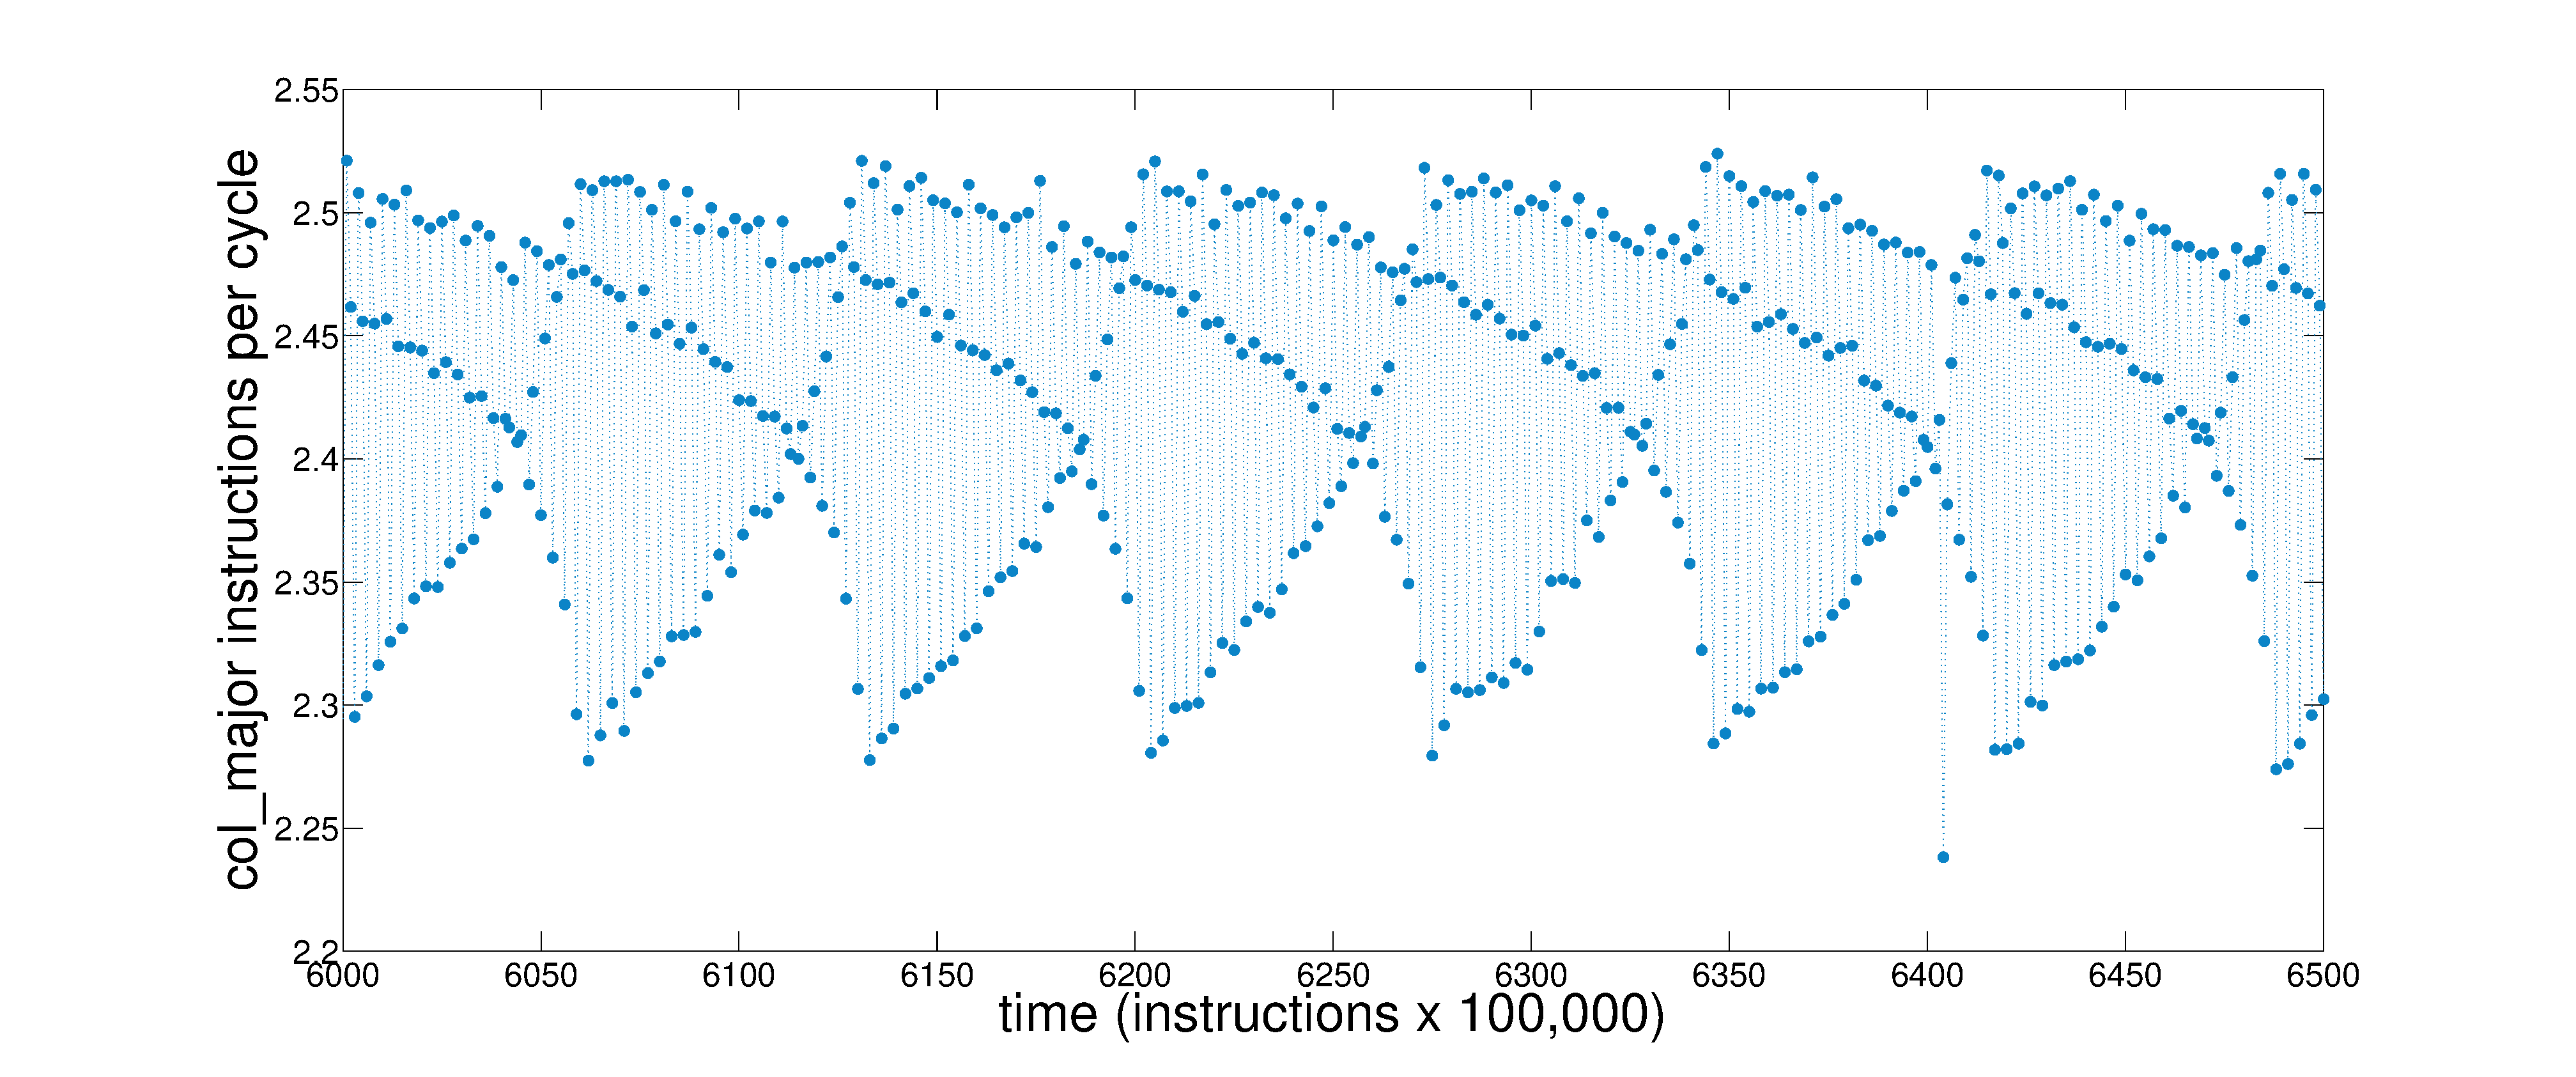
\includegraphics[width=\textwidth]{figs/colshortts}
    % where an .eps filename suffix will be assumed under latex,
    % and a .pdf suffix will be assumed for pdflatex
    \caption{A small snippet of the instructions per cycle(ipc) of {\tt
        \col}, a three-line C program that repeatedly initializes
      a matrix in column-major order, running on an Intel i7\textsuperscript{\textregistered}-based machine.  Even this
      simple program exhibits chaotic performance dynamics.}
   \label{fig:ipc}
  \end{figure}









The computer systems community has applied a variety of prediction
strategies to traces like this, most of which employ regression.  An
appealing alternative builds on the recently established fact that
computers can be effectively modeled as deterministic nonlinear
dynamical systems \cite{mytkowicz09}.  This result implies the
existence of a deterministic forecast rule for those dynamics.  In
particular, one can use \emph{delay-coordinate embedding} to
reconstruct the underlying dynamics of computer performance, then use
the resulting model to forecast the future values of computer
performance metrics such as memory or processor loads
\cite{josh-ida2011}.  In the case of simple microkernels like the one
that produced the trace in Figure~\ref{fig:ipc}, this deterministic
modeling and forecast strategy works very well.  In more-complicated
programs, however, such as speech recognition software or compilers,
this forecast strategy---as well as the traditional methods---break
down quickly.

This paper is a first step in understanding when, why, and how
deterministic forecast strategies fail when they are applied to
deterministic systems.  We focus here on the specific example of
computer performance.  We conjecture that the complexity of traces
from these systems---which results from the inherent dimension,
non-linearity, and non-stationarity of the dynamics, as well as from
measurement issues like noise, aggregation, and finite data
length---can make those deterministic signals \emph{effectively}
unpredictable.  We argue that \emph{permutation entropy}
\cite{bandt2002per}, a method for measuring the entropy of a
real-valued-finite-length time series through ordinal analysis, is an
effective way to explore that conjecture.  We study four
examples---two simple microkernels and two complex programs from the
SPEC benchmark suite---running on different Intel-based machines.  For
each program, we calculate the permutation entropy of the processor
load (instructions per cycle) and memory-use efficiency (cache-miss
rates), then compare that to the prediction accuracy attainable for
that trace using a simple deterministic model.

% paragraph to appease the theoretician in me
It is worth taking a moment to consider the theoretical possibility of
this task. We are not attempting to predict the state of the CPU at an
arbitrary point in the future --- this, at least with perfect
accuracy, would be tantamount to solving the halting problem. What we
are attempting is to predict aspects or functions of the running of
the CPU: instructions executed per second, cache misses per 100,000
instructions, and similar statistics. Prediction of these quantities
at some finite time in the future, even with perfect accuracy, does
not violate the Rice-Shapiro theorem.

% The rest of the paper is organized as follows.
% Section~\ref{sec:compModel} describes the experimental setup, as well
% as the nonlinear modeling and forecast strategies.  In
% Section~\ref{sec:meaComplex}, we review permutation entropy, calculate
% its value for a number of different computer performance traces, and
% compare the results to the prediction accuracy.  In
% Section~\ref{sec:conc}, we discuss these results and their
% implications in regard to our conjecture, and consider future areas of
% research.


\section{Related Work}\label{sec:related}

Attempting to model and characterize predictability is a very old problem which arguably began with Yule in 1927 when he invented AR and many attempts to quantify predicatbility have followed including ....

Entropy though Generating partitions 
works **if** you have generating parition but not if you don't
{\color{blue} Ryan: Please insert here the paragraph and citations defaming binning / partitioning and illustrating the difficulty of generating partitions / biasing of this method without generating partitions, along with relevant citations. }


Redundancy (details in SFI forecasting), relies heavily on either estimating the generating partiion which is hard to do *and* estimating the positive lyap spectrum which is hard to do for noisy systems and impossible for systems that are not deterministic. 

DVS plots, gives pros and cons in (SFI prediction book)

predicting local predictive capacity (radial basis functions stuff, trying to predict error bounds on next forecast based on ensemble uncertainty) but does not aggregate tell you at what level the time series exhibits complexity only locally predictive structure, this actualy gets at the interesting point that different regions of a time series may exhibit differnt levels of complexity which we will illustrate with \svd

Distrubtion of error. For many methods, if your error is not normally distributed this signals that there is stil more predictve structure to that could be used by for example a larger order ARMA process. But if error is normally distributed, this suggests that you have used up all the predictive structure that **that** model can use, this doesn't quantify if preidctuce structure exists that isn't being used by this process. For example, nonlinear structure which is ignored by a linear predictor. 


But this method is differnt becasue it uses no assumption about the underlying model, does not require generating partitions, is applicable to noisy real-valued time series. 


Maybe talk about ``
wpe has been applied to predicting irregularities in brain wave data but no on one has examined it's correlation with predictive structure. "
but kind of puts the cart before the horse



\section{Experimental Methods and Time Series Explanations}

 \begin{enumerate}
 \item  Experimental methods: (how we collect the time series and what the times series areThis should be HPM PAPI, which programs we model
\item programs 
\subitem description of \col
\subitem description of \gcc
\subitem description of \svd 
\subitem description of svd regimes
 \end{enumerate}


\subsection{Time Series Collection}

The time-series data for these experiments was collected on an Intel Core\textsuperscript{\textregistered} i7-2600 running the 2.6.38-8 Linux
kernel.  This Nehalem chip has eight cores running at 3.40GHz and a cache size
of 8192 KB.  We studied three example programs---a simple microkernel(\col) and two complex programs: one from the
SPEC 2006CPU benchmark suite(\gcc), and one from LAPACK(\svd), aggregating and measuring the processor load---instructions per cycle (ipc)---at 100,000-instruction intervals.  To record these measurements,
we used the {\tt libpfm4}, via PAPI
\footnote{Performance Application Programming Interface}\cite{papi-website}, which we have instrumented to stop program execution every 100,00-instructions and read the contents of the CPU's onboard hardware performance monitors (HPMs). HPMs are specialty registers built for this purpose. Obviously using a system to measure itself can cause interference but due diligence was put into monitoring the generating process of these time series without interfering with it in a significant way. For an in-depth explanation of this custom-measurement infrastructure as well as discussion on choice of interrupt rate see 
\cite{zach-IDA10,mytkowicz09,todd-phd}.



\subsection{The Programs}
We study three example programs---a simple microkernel(\col) and two complex programs: one from the
SPEC 2006CPU benchmark suite(\gcc), and one from LAPACK(\svd).
\subsubsection{\col}
\col is a simple three-line C program that repeatedly initializes the top half of matrix in column-major order. While this is a very simple program it has been shown to exhibit very complicated behavior. In fact, in \cite{chaos} it was shown 
\subsubsection{\gcc}

\subsubsection{\svd}
\svd brings up a very interesting point: systems change over time. While it is clear in Figure \ref{fig:sample-ts} (a) and (b) that a single system is being observed, it also appears \emph{visually} that the complexity of these two time series is consistent over time, i.e., while they are both complicated they don't appear to increase or decrease in complexity over the range of the program. \svd (seen in Figure \ref{fig:svd-ts-colored}) is different however, at least visually. Figure \ref{fig:svd-ts-colored} is a single trace of \svd from start to finish, however as time progresses it is clear that something drastically changes in the underlying generating process and the structure of the time series is visually very different from section to section. This is caused by the code of \svd moving between different subroutines. We call these changes in \svd dynamics  \emph{\svd regimes} and we have colored each of the six regimes different colors in Figure \ref{fig:svd-ts-colored}. The advantage to splitting \svd into these regimes is to explore how complexity and predictability evolve over time for a system in drift. In Section \ref{sec:wpeRegime} we explore and validate the choice of these visually selected regime windows extending techniques from \cite{cao2004det}. The purpose of this paper is not to rigorously explore regime detection but to explore quantifying complexity of a time series. As such, making this split simply serves as providing 90 unique time series\footnote{Six Regimes with 15 individual runs each.} to explore. For notational convience we refer to these signals as {\tt dgesdd$_i$} with $i \in \{1\dots6\}$ where $i$ corresponds to a regime of \svd. The regimes are labeled from left to right. 



\begin{figure}[htbp]
  \centering
  \begin{subfigure}[t]{\textwidth}
  \centering
    \includegraphics[width=0.75\textwidth]{figs/colFullTS}
    \caption{\col Time Series}
    \label{fig:col-ts}
  \end{subfigure}%
  \\
  
  \begin{subfigure}[t]{\textwidth}
  \centering
    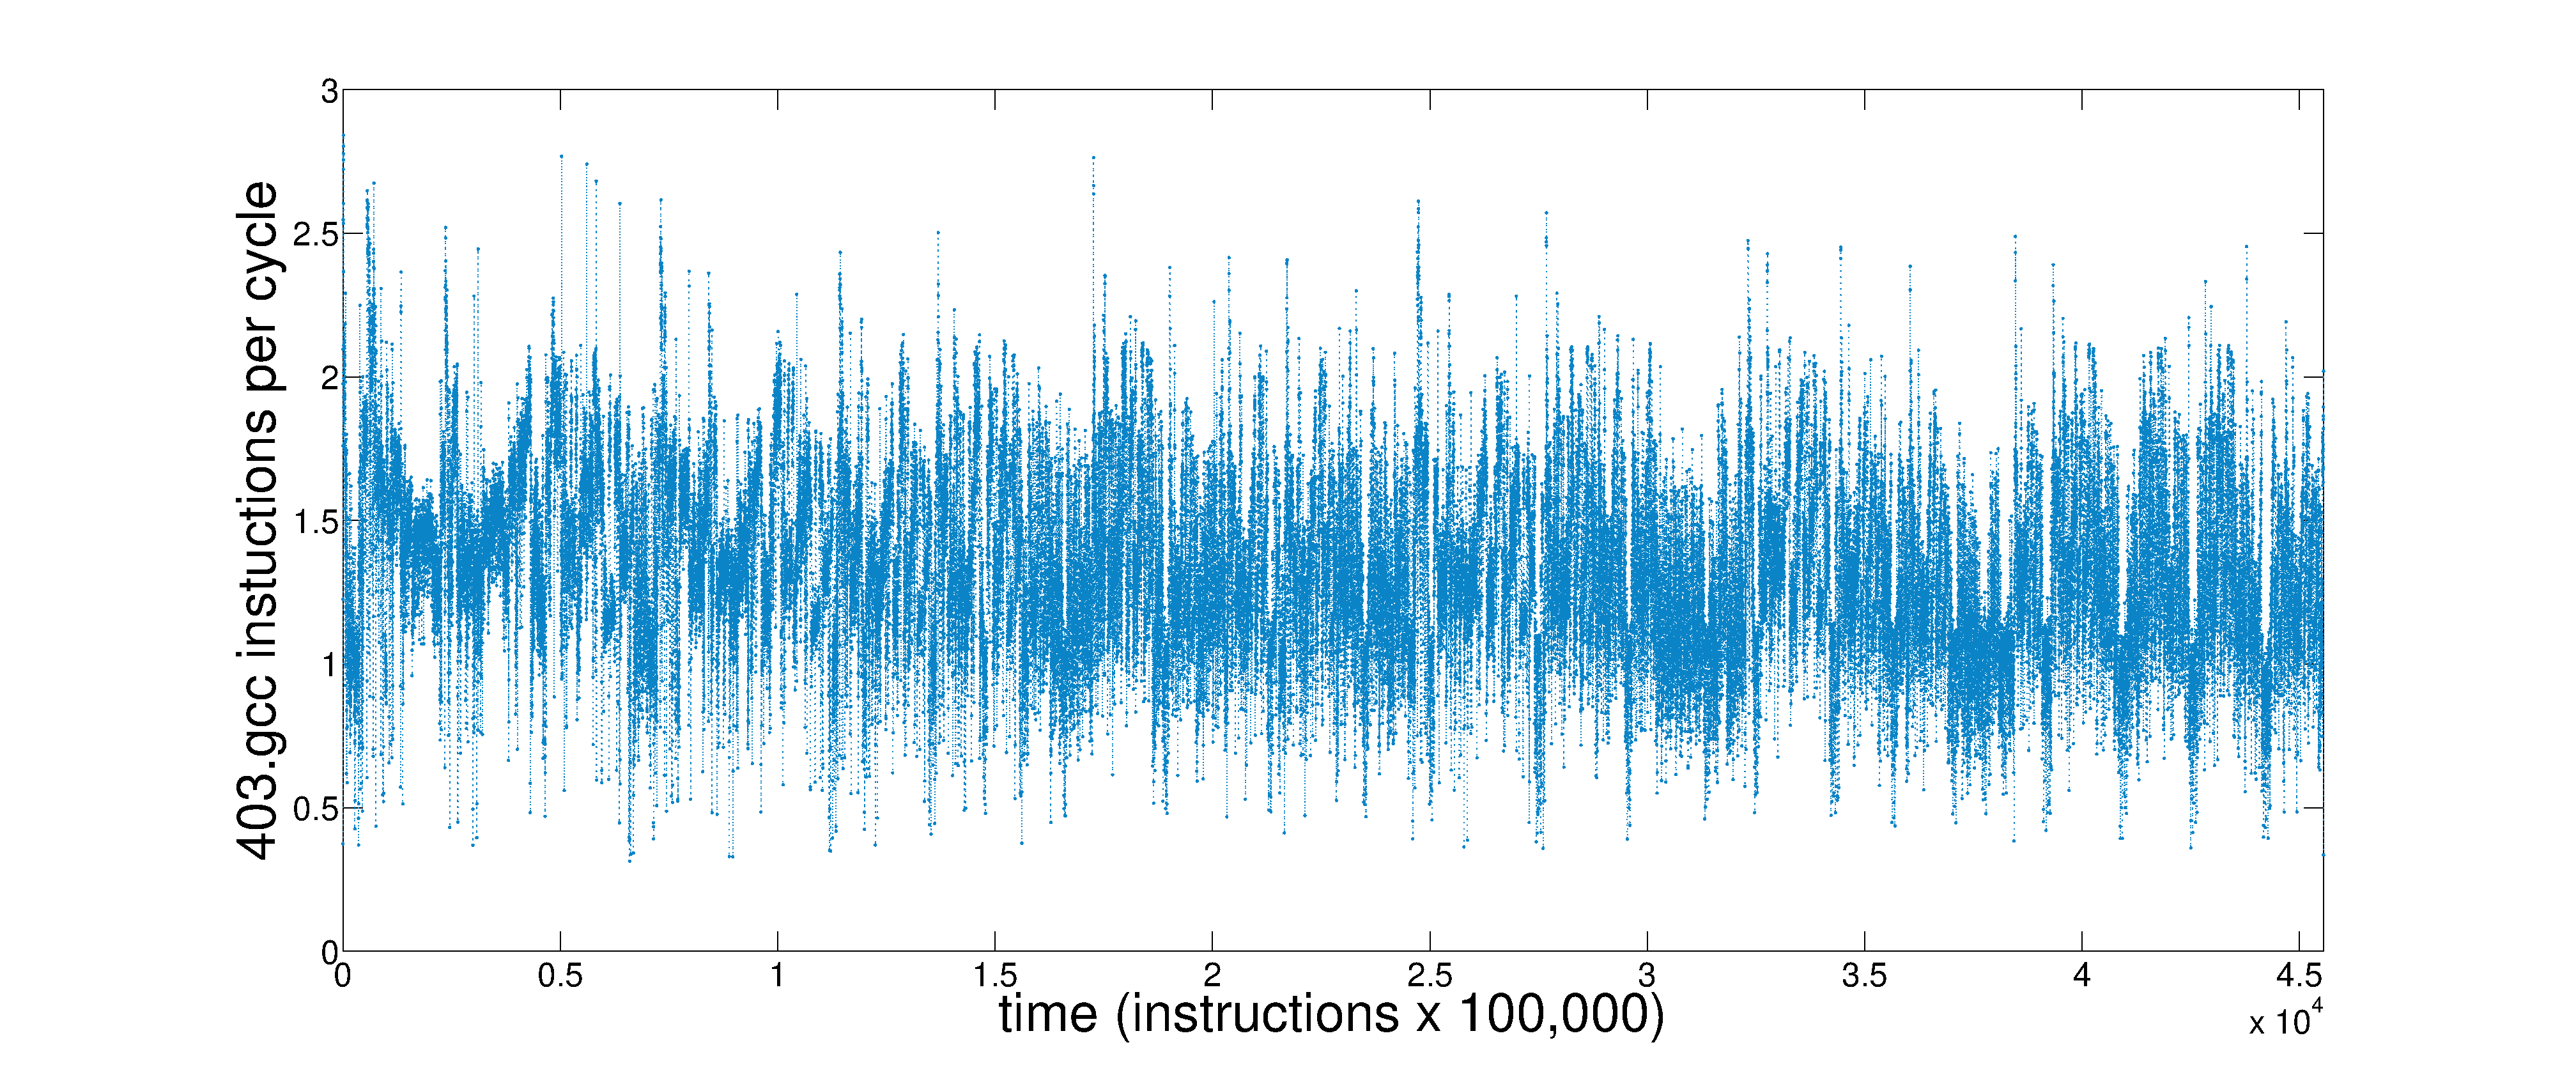
\includegraphics[width=0.75\textwidth]{figs/gccfullts}
    \caption{\gcc Time Series}
    \label{fig:gcc-ts}
  \end{subfigure}
    \begin{subfigure}[t]{\textwidth}
    \centering
    \includegraphics[width=0.75\textwidth]{figs/SVD1RegimesColored}
    \caption{\svd Time Series with Regime Coloring}
    \label{fig:svd-ts-colored}
  \end{subfigure}
  \caption{[[Maybe this should be just a picture of each time series and then have another figure with color after explaining heuristically the reigmes. In (a) the instructions executed per CPU clock cycle
    (IPC) during the execution of \col. Each point is the average IPC during a 100,000
    instruction period. Similarly in (b) is a time series of the IPC during the execution of \gcc.}\label{fig:sample-ts}
    \end{figure}


\section{Modeling }\label{sec:model}
%
% {\color{blue} EDITABLE}
%
% Section outline:
%
% \begin{enumerate}
% \item \cmark section intro
% \item \cmark fix order from simplest to most complex
% \item Description of DCE and parameter estimation
% \item\cmark Description of auto ARIMA
% \item \cmark Description of the two naive methods (random walk and mean), make sure to explain that these methods are naive and simple but not necessarily bad.
% \item\cmark Add a section talking about evaluation methods i.e., MASE, this text is currently written and just sitting at the beginning of the results.
%
% \end{enumerate}

In this section, we describe the four different forecasting methods
used in this study, as well as the error metric used to evaluate their
predictive accuracy.  These methods include:
\begin{itemize}
\item The \emph{random-walk} method, which uses the previous value in
  the observed signal as the forecast,

\item The \emph{\naive} method, which uses the mean of the
  observed signal as the forecast,

\item The \emph{ARIMA} (auto-regressive integrated moving average)
  method, a common linear forecast strategy, built using the
  \emph{\arima} procedure \cite{autoARIMA}, and

\item The \emph{LMA} (Lorenz method of analogues) method, which uses a
  near-neighbor forecast strategy on a dynamical reconstruction of the
  signal.
\end{itemize}
ARIMA models are based on standard autoregressive techniques.  LMA is
designed to capture and exploit the deterministic structure of a
signal from a nonlinear dynamical system.  The \naive ~and random-walk
methods, somewhat surprisingly, often outperform these
more-sophisticated prediction strategies in the case of highly complex
signals, as discussed below.

These four forecast methods were chosen to be a representative
sampling of standard prediction strategies, but they do not, of
course, cover that space exhaustively.  Our goal here is an empirical
assessment of the relationship between predictability and complexity,
not formal results about a ``best'' predictor for a given time series.
From a practitioner's standpoint, it would be useful to know \emph{ a
  priori} if a time series contains enough predictive structure to
make it worth spending the time and effort searching for a good
forecast method.  It would also be useful to know if a given method is
inadequate---that is, if an alternative method could do better and so
one should continue searching.  \alert{need to check that this is not
  redundant, given the other text in this section (and elsewhere in
  the paper).  it may be better to put this in the conclusion.}

\subsection{Two Simple Prediction Strategies}
\label{sec:simple}

A random-walk predictor simply uses the last observed measurement as
the forecast: that is, the predicted value $p_i$ at time $i$ is
calculated using the following relation: $$p_i = x_{i-1}$$ The
prediction strategy that we refer to using the term ``\naive''
averages the prior observations to generate the forecast: $$p_i =
\sum_{j=1}^{i-1}\frac{x_j}{i-1}$$ While both of these methods are
simplistic, they are not without merit.  For a time series near the
high end of the complexity spectrum---i.e., one that possesses very
little predictive structure---these two methods can actually be the
best choice.  In forecasting currency exchange rates, for instance,
sophisticated econometrics-based prediction models fail to
consistently outperform the random-walk method~\cite{rwMeese,rwCCE}.
These signals are constantly changing, noisy, and possess very little
predictive structure, but their variations are not---on the
average---very large, so the random-walk method's strategy of simply
guessing the last known value is not a bad choice.  If a signal has a
unimodal distribution with low variance, the \naive ~prediction
strategy will perform quite well---even if the signal is highly
complex---simply because the mean is a good approximation of the
future behavior.  Moreover, the \naive ~prediction strategy's temporal
average effects a low-pass filtering operation, which can  mitigate the
complexity in signals with very little predictive structure.

Both of these methods have significant weaknesses, however.  Because
they do not model the temporal patterns in the data, or even the
distribution of its values, they cannot track changes in that
structure.  This causes them to fail in a number of important
situations.  Random-walk strategies are a particularly bad choice for
time series that change significantly at every time step.  In the
worst case---a large-amplitude square wave whose period is equivalent
to twice the sample time---a random-walk prediction would be exactly
180 degrees out of phase with the true continuation.  The \naive
~method would be a better choice in this situation, since it would
always split the difference.  It would, however, perform poorly when a
signal has a number of long-lived regimes that have significantly
different means.  In this situation, the inertia of the \naive
~method's accumulating mean is a liability and the agility of the
random-walk method is an advantage, since it can respond quickly to
regime shifts.

Of course, methods that could capture and exploit the geometry of the
data and/or its temporal patterns would be far more effective in the
situations described in the previous paragraph.  The \arima and LMA
methods introduced in Sections~\ref{sec:arima} and~\ref{sec:lma} are
designed to do exactly that.
% Note, though, that periodic patterns
%appear only in signals that are at the low end of the %complexity
%spectrum.
However, if a signal contains little predictive structure, forecast
strategies like ARIMA and LMA have nothing to work with and thus will
often be outperformed by the two simple strategies described in this
section.  This effect is explored further in Sections~\ref{sec:accuracy}
and~\ref{sec:results}.


\subsection{A Regression-Based Prediction Strategy}
\label{sec:arima}
%\begin{enumerate}
%\item\cmark introduce method abstractly and practically, common method basically fitting a hyperplane to data removing seasonality and filtering for noise
%\item\cmark define rigorously, all the backshift operator garbage

%$$\Phi(B^m)\phi(B)(1-B^m)^D(1-B)^dX_i = c + \Theta(B^m)\theta(B)\epsilon_i$$

%$$B^mX_i  = X_{i-m}$$
%\item\cmark discuss that this method needs linear structure to work correctly
%\item \cmark maybe talk about converging to zero and limits on prediction horizon
%\end{enumerate}

%For this \cite{davislinearts}

%%%%%%%%%%%%%%%%%%%%%%%%%%%%%%%%%%%%%%%%%%%%%%%%%%%%%%%%%%%%%%%%%%%%%%%%%
% here is the old version of this material, for use in other documents...
%
%Perhaps the simplest way to capture and exploit the structure of data
%is to fit a hyperplane to the dataset and then use that it to forecast
%new data points.  The roots of this date back to Yule's 1927 invention
%of the autoregressive schema~\cite{weigend93}, which forecasts the
%next time step through a weighted average of past observations: $$p_i
%= \phi(B^p)x_{i}$$ where $\phi(\cdot)$ is a polynomial of degree $p$
%that is fit to the past $p+1$ [???] values of $x_i$ via the
%backshift operator $B$ \footnote{I changed the superscript to $k$ to
%  make this definition general---not connected to any of the terms
%  that have specific meanings later in this section.}:
%$$B^k x_i = x_{i-k}$$
%%
%with $k=1...p$.  To account for noise in the data, one can add a
%so-called ``moving average'' term to the model:
%$\theta(B^q)\epsilon_i$, where $\theta(\cdot)$ is a polynomial of
%degree $q$ and $\epsilon$ is white noise with the same mean and
%variance as the data.
%% if you leave this in, you'll need to explain a lot about the data
%% and the calculation
%% $\{\epsilon_i\}\sim WN(0,\sigma^2)$.
%To remove nonstationarities in the data, one can detrend it using a
%differencing operation: $(1-B^d)x_i$.
%
%A strategy that incorporates all three of these features is called a
%\emph{nonseasonal ARIMA} model of order $(p,d,q)$:
% $$\phi(B^p)(1-B^d) x_i = \theta(B^q)\epsilon_i$$
%%
%{\color{red} You had superscripts on some of the $B$s and not on
%  others.  I added them but I may have gotten them wrong.  I also
%  changed some $(1-B)^d$s to $(1-B^d)$s to make things consistent with
%  the first use of that construction.  Please make sure things are
%  consistent, here and throughout this section.}  Here, $p$, $d$ and
%$q$ correspond to the orders of the autoregressive, detrending, and
%moving average terms, respectively.
%
%If periodic structure is present in the data, a \emph{seasonal ARIMA}
%model of order $(p,d,q)(P,D,Q)$ can be a good choice:
%%
%$$\Phi(B^P)\phi(B^p)(1-B^m)^D(1-B^d) x_i =
%\Theta(B^Q)\theta(B^q)\epsilon_i$$
%%
%Here $\Phi(\cdot)$ and $\Theta(\cdot)$ are polynomials of degree $P$
%and $Q$, respectively [which accomplish what purpose?  why?  how?
%    where did $D$ come from and what does it do?].  $m$ is the
%seasonal frequency [shouldn't this be ``period''?].  [Explain why
%    one should choose $P=Q=m$, since that's what the equation below
%    implicitly does.]  To use a seasonal ARIMA model, one first uses
%the detrending term to remove nonstationarity: $$\hat{x_i} =
%(1-B^m)^D(1-B^d) x_{i}$$ and then creates the forecast $p_i$ by
%evaluating $$\Phi(B^m)\phi(B^p)\hat{X_i} =
%\Theta(B^m)\theta(B^q)\epsilon_i$$
% ...down to here
%%%%%%%%%%%%%%%%%%%%%%%%

A simple and yet powerful way to capture and exploit the structure of
data is to fit a hyperplane to the known points and then use it to
make predictions.  The roots of this approach date back to the
original autoregressive schema~\cite{weigend93}, which forecasts the
next time step through a weighted average of past observations: $$p_i
= \sum_{j=1}^{i-1} a_j x_j$$ The weighting coefficients $a_j$ are
generally computed using either an ordinary least squares approach, or
with the method of moments using the Yule-Walker equations.  To
account for noise in the data, one can add a so-called ``moving
average'' term to the model; to remove nonstationarities, one can
detrend the data using a differencing operation.  A strategy that
incorporates all three of these features is called a \emph{nonseasonal
  ARIMA model}.  If evidence of periodic structure is present in the
data, a \emph{seasonal ARIMA model}, which adds a sampling operation
that filters out periodicities, can be a good choice.

There is a vast amount of theory and literature regarding the
construction and use of models of this type; we refer the reader to
\cite{davislinearts} for an in-depth exploration.  For the purposes of
this paper, where the goal is to explore the relationship between
predictability and complexity across a broad array of forecast
strategies, seasonal ARIMA models are a good exemplar of the class of
linear predictors.  Fitting such a model to a dataset involves
choosing values for the various free parameters in the autoregressive,
detrending, moving average, and filtering terms.  We employ the
automated fitting techniques described in~\cite{autoARIMA} to
accomplish this, producing what we will call an ``\arima model''in the
rest of this paper.  This procedure uses sophisticated methods---KPSS
unit-root tests~\cite{KPSSunit}, a customization of the Canova-Hansen
test~\cite{Canova1995}, and the Akaike information
criterion~\cite{akaike1974}, conditioned on the maximum likelihood of
the model fitted to the detrended data---to select good values for the
free parameters of the ARIMA model.

ARIMA forecasting is a common and time-tested procedure.  Its
adjustments for seasonality, nonstationarity, and noise make it an
appropriate choice for short-term predictions of time-series data
generated by a wide range of processes.  If information is being
generated and/or transmitted in a nonlinear way, however, a global
linear fit is inappropriate and ARIMA forecasts can be inaccurate.
Another weakness of this method is prediction horizon: an ARIMA
forecast is guaranteed to converge (to the mean, to a constant value,
or to a linear trend) after some number of predictions, depending on
model order.  To sidestep this issue, we build forecasts in a stepwise
fashion: i.e., fit the \arima model to the existing data, use that
model to perform a one-step prediction, rebuild the \arima model using
the latest observations, and iterate until the desired prediction
horizon is reached.  For consistency, we take the same approach with
the other three models in this study as well, even though doing so
amounts to artificially hobbling LMA.

\subsection{A Nonlinear Prediction Strategy}
\label{sec:lma}

When the temporal progressions in a time series are produced by a
deterministic nonlinear process, one can use a technique called
delay-coordinate embedding
%
%% Note: claiming that we can reconstruct the dynamics of the
%% underlying generating process isn't right.  That would be
%% equivalent to solving the system identification problem!  We're
%% not reconstructing the underlying system, just its output.
%
to model the structure of the information generation and transmission
occurring in the underlying process, then use that reconstruction to
generate forecasts.  This section discusses the theory and
implementation of a prediction strategy that is based on this idea.

Delay-coordinate embedding~\cite{packard80,Sauer:1991lr,Takens:1981uq}
allows one to reconstruct a dynamical system's full state-space
dynamics from a scalar time-series measurement---provided that some
conditions hold regarding those data.  Specifically, if the underlying
dynamics and the measurement function---the mapping from the unknown
state vector $\vec{X}$ to the observed value $x_i$---are both smooth
and generic, Takens~\cite{Takens:1981uq} formally proves that the
delay-coordinate map
\[
F(\tau,m)(\vec{X}) = ([x_{i} ~ x_{i+\tau} ~ \dots ~x_{i+m\tau}])
\]
from a $d$-dimensional smooth compact manifold $M$ to
$\mathbb{R}^{2d+1}$ is a diffeomorphism on $M$: in other words, that
the reconstructed dynamics and the true (hidden) dynamics have the
same topology.  This is an extremely powerful result; among other
things, it means that one can model the full system dynamics, up to
diffeomorphism, without measuring---or even knowing---anything about
the state variables.

The first step in the delay-coordinate embedding process is to
estimate values for the two free parameters in the map: the delay
$\tau$ and the dimension $m$.  We follow standard procedures for this,
choosing the first minimum in the time-delayed mutual information as
an estimate of $\tau$~\cite{fraser-swinney} and using the
false-near(est)-neighbor method of~\cite{KBA92} to estimate $m$.  Some
example plots of data from
Figures~\ref{fig:col-ipc}-\ref{fig:svd-ts-colored}, embedded following
this procedure, are shown in Figure~\ref{fig:embedding}.
% \begin{figure}
%   \centering
%\begin{subfigure}{\columnwidth}
%    \includegraphics[width=\columnwidth]{figs/colipc3d}
%    \caption{\col }
%    \label{fig:colEmbedding}
%  \end{subfigure}%  \\
%
%    \begin{subfigure}{\columnwidth}
%    \includegraphics[width=\columnwidth]{figs/gcc3dipc}
%    \caption{\gcc}
%    \label{fig:gccEmbedding}
%  \end{subfigure}
%  \\
%  \begin{subfigure}{\columnwidth}
%    \includegraphics[width=\columnwidth]{figs/svd53dipc2}
%    \caption{\svdfive}
%    \label{fig:svdfiveEmbedding}
%  \end{subfigure}%
%%
%
%
%     %\includegraphics[width=\textwidth]{colipc3d}
%     \caption{3D projections of delay-coordinate embeddings of the
%       traces from (a) Figure~\ref{fig:col-ts} (b)
%       Figure~\ref{fig:gcc-ts} and (c) the fifth (green) segment of
%       Figure~\ref{fig:svd-ts-colored}.}
% \label{fig:embedding}
% \end{figure}
 \begin{figure}[!ht]
    \subfloat[\col\label{fig:colEmbedding}]{%
      \includegraphics[width=\columnwidth]{figs/colipc3d}
    }
    \hfill
    \subfloat[\gcc\label{fig:gccEmbedding}]{%
      \includegraphics[width=\columnwidth]{figs/gcc3dipc}
    }
        \hfill
    \subfloat[\svdfive \label{fig:svdfiveEmbedding}]{%
      \includegraphics[width=\columnwidth]{figs/svd53dipc2}
    }
    \caption{3D projections of delay-coordinate embeddings of the
       traces from (a) Figure~\ref{fig:col-ipc} (b)
       Figure~\ref{fig:gcc-ts} and (c) the fifth (green) segment of
       Figure~\ref{fig:svd-ts-colored}.}
    \label{fig:embedding}
  \end{figure}
%% can cut for space if need be:
%The coordinates of each point in these plots are differently delayed
%elements of the instructions per cycle time series $X_{i,obs}$: that
%is, $X_{i,obs}$ on the first axis, $X_{i+\tau,obs}$ on the second,
%$X_{i+2\tau,obs}$ on the third, and so on.
%

Geometric structure in these kinds of plots is an indication of
structure in the information generation/transmission process that
produced the time series.  The dynamical systems community has
developed a number of methods that leverage this structure to generate
predictions (e.g.,~\cite{weigend-book,casdagli-eubank92,Smith199250}).
One of the most straightforward of these is the \emph{Lorenz method of
  analogues} (LMA), which is essentially nearest-neighbor prediction
in the embedded\footnote{Lorenz's original formulation used the full
  system state space;
%
%According to \cite{kantz97},
%
this method was first extended to embedded dynamics by
Pikovsky~\cite{pikovsky86-sov}, but is also related to the prediction
work of Sugihara \& May~\cite{sugihara90}}
space~\cite{lorenz-analogues}.  Even this simple algorithm---which
builds predictions by finding the nearest neighbor in the embedded
space of the given point, then taking that neighbor's path as the
prediction---provides accurate forecasts when the generating process
is a deterministic dynamical system.

Since LMA does not rest on an assumption of linearity (as ARIMA models
do), it can handle both linear and nonlinear processes.  If the
underlying generating process is nondeterministic, however, it can
perform poorly.  Figure~\ref{fig:embedding}(b), for instance, appears
to contain little structure, so LMA may not work well on this signal.
More structure appears to be present in Figure~\ref{fig:embedding}(c),
but this reconstruction also appears to contain some noise.  The
question as to how much structure is present in a reconstruction, and
how much of that structure can be captured and used by LMA, is apropos
of the central question treated in this paper.  It may be that \gcc
has some redundancy that LMA cannot exploit, or that the structure in
\svdfive is effectively obfuscated, from the standpoint of the LMA
method, by noise.  Without any knowledge of the generating process,
answers to these questions can only be derived from the data, with all
of the attendant problems (noise, sampling issues, and so on).  By
quantifying the balance between redundancy, predictive structure, and
entropy for these real-valued time series---as shown in
Section~\ref{sec:results}---we can begin to answer these questions in
an effective and practical manner.

% If enough predictive structure is present in these embeddings, that
% structure can be used to build an effective forecast model.

\subsection{Assessing Prediction Accuracy}
\label{sec:accuracy}

To study the relationship between predictability and complexity, we
use the four methods outlined above to generate predictions of all 120
traces described in Section~\ref{sec:methods}, then calculate the
error of the predictions with respect to the true continuations.
Specifically, we split each time series into two pieces: the first
90\%, referred to as the ``initial training" signal and denoted
$\{x_i\}_{i=1}^{n}$, and the last 10\%, known as the ``test" signal
$\{c_j\}_{j=n+1}^{k+n+1}$.  The initial training signal is used to
build the model, following the procedures described in the previous
section; that model is used to generate a prediction of the value of
$x_{n+1}$, which is then compared to the true continuation, $c_{n+1}$.
The model is then rebuilt using $\{x_i\}_{i=1}^{n+1}$ and the process
repeats $k$ times, out to the end of the observed time series.  This
``one step prediction'' process is not technically necessary in the
LMA method, whose ability to generate accurate predictions is limited
only by the positive Lyapunov exponents of the system.  However, the
performance of the other three methods used here will degrade severely
if the associated models are not periodically rebuilt.  In order to
make the comparison fair, we used an iterative one-step prediction
schema \emph{for all four methods}.  This has the slightly confusing
effect of causing the ``test'' signal to be used both to assess the
accuracy of each model and for periodic refitting.

Figure~\ref{fig:forecast-example} shows example forecasts made using
all four methods for the \col, \gcc, and \svdfive time series.
%\begin{figure*}[htbp]
%  \centering
%
%  \begin{subfigure}{0.6\columnwidth}
%    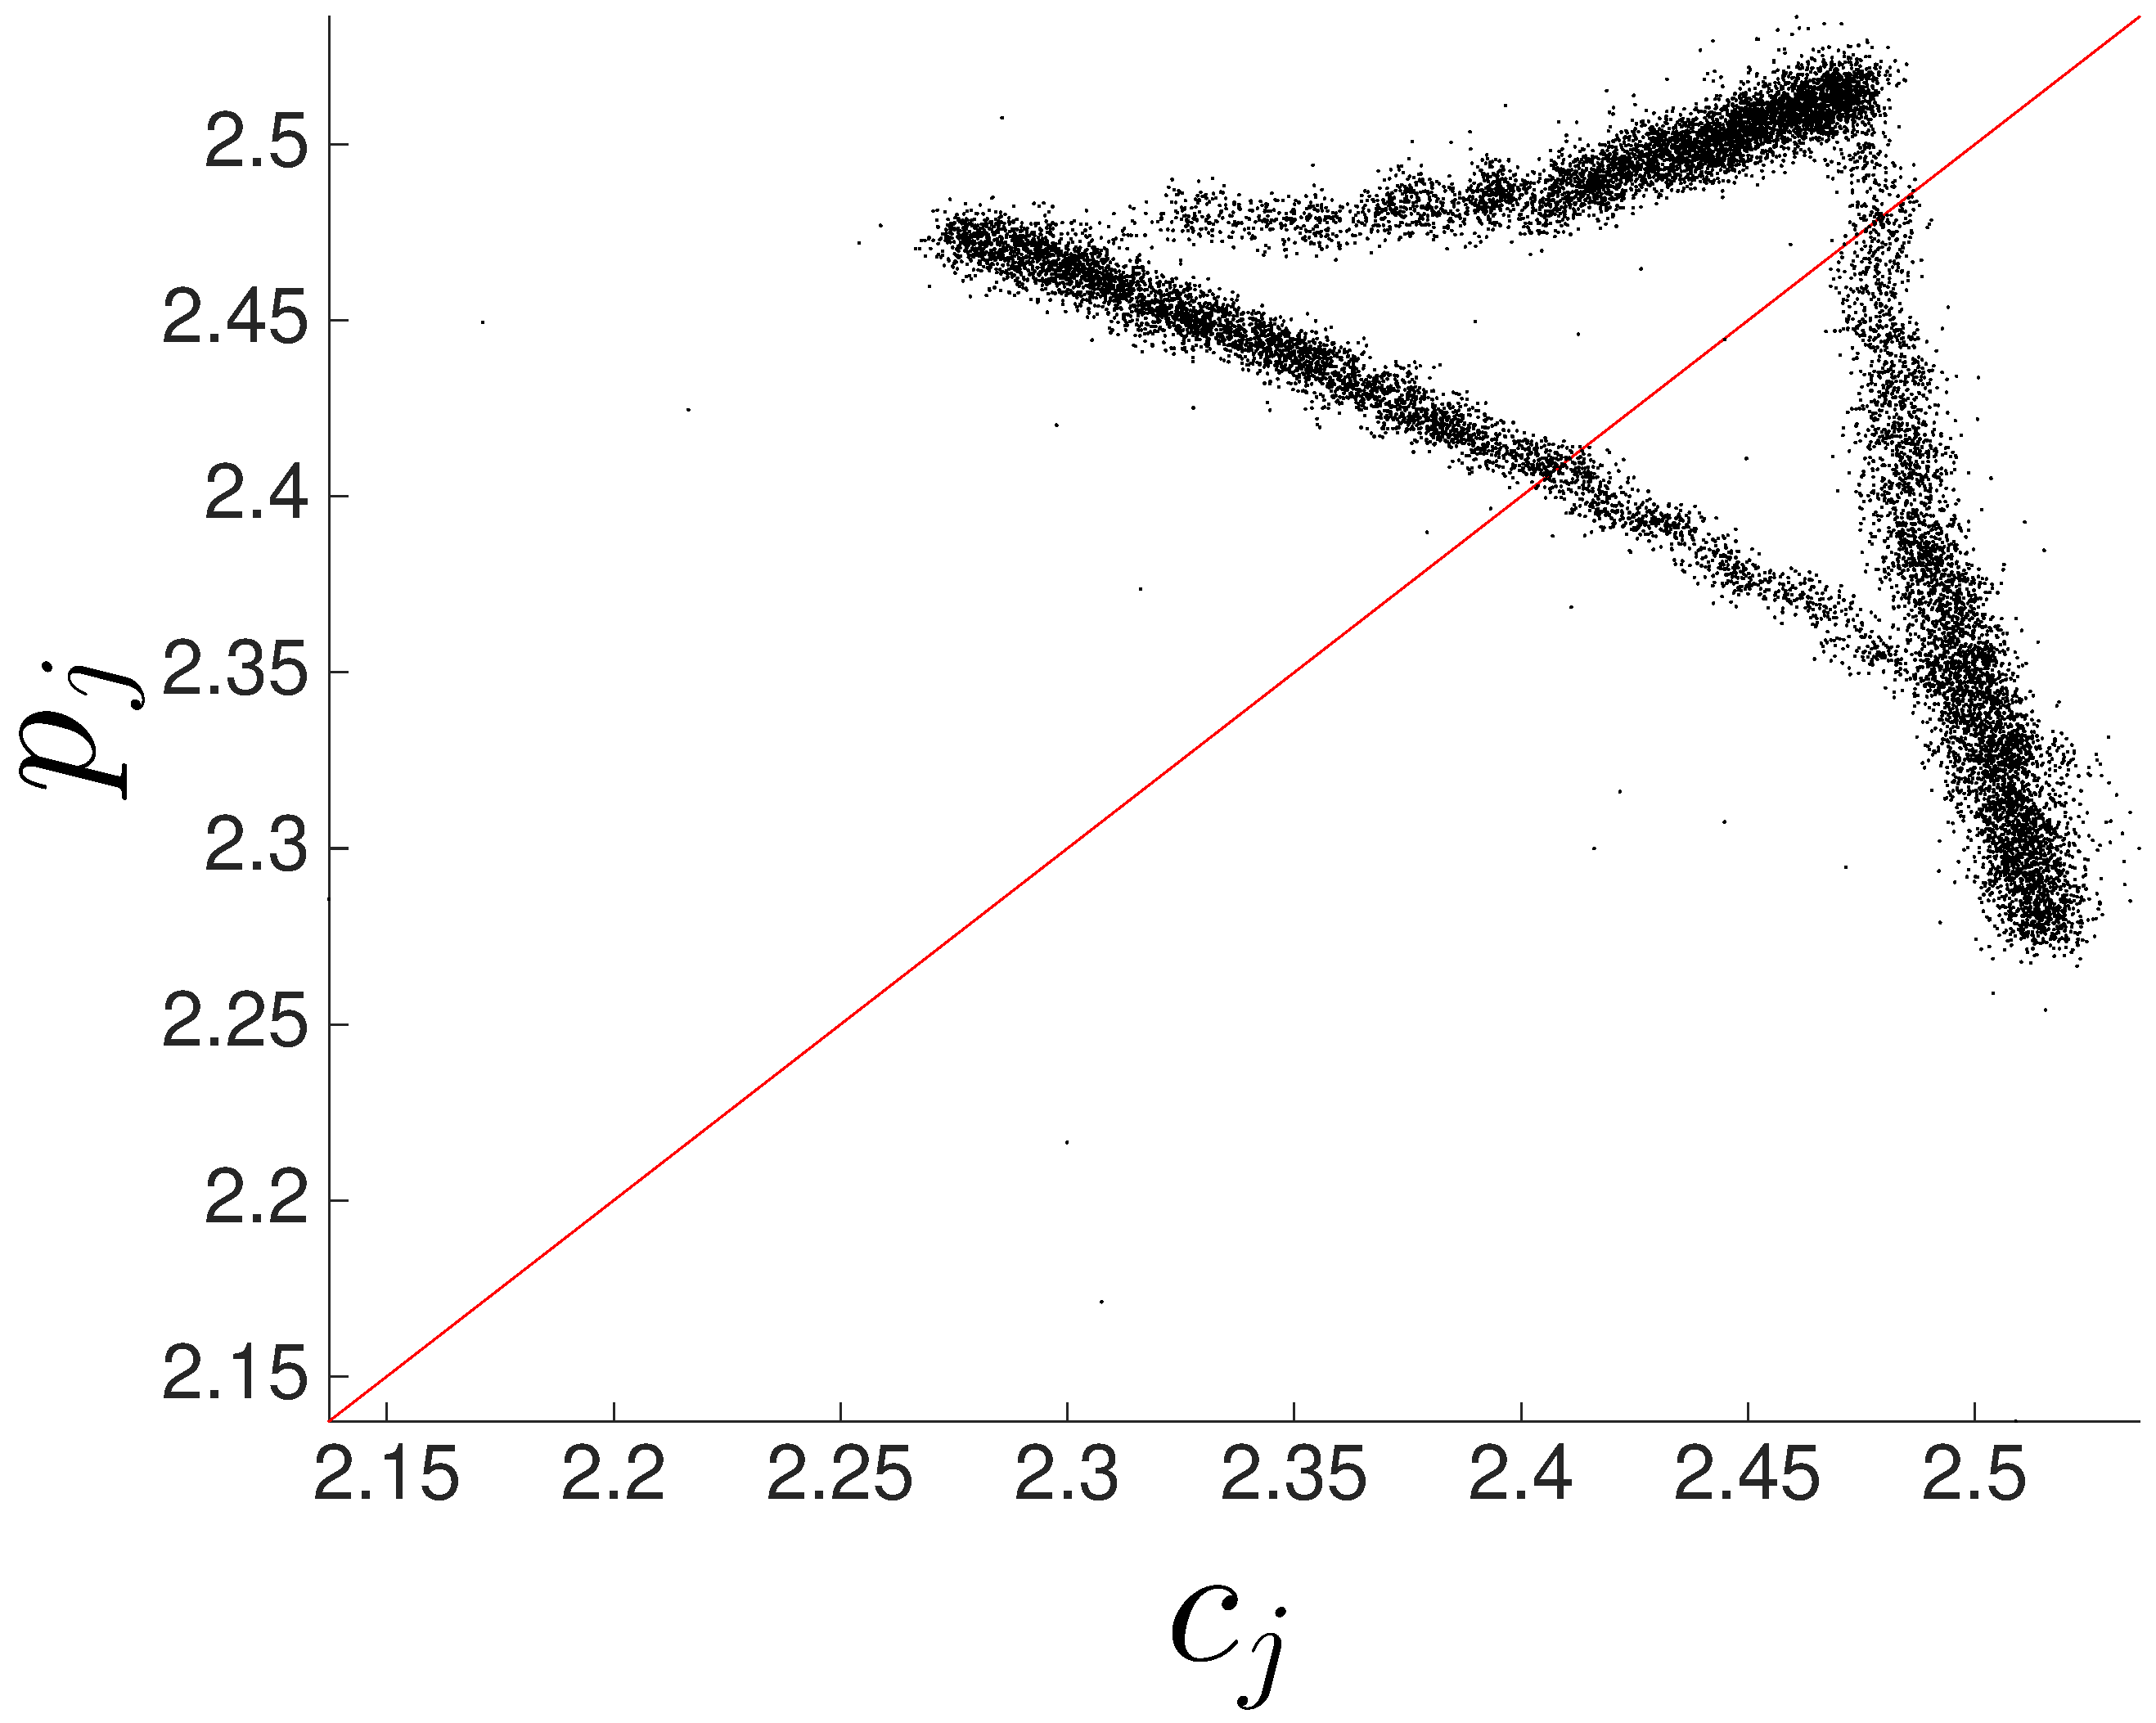
\includegraphics[width=\columnwidth]{figs/colRWForecast}
%    \caption{\col\\ random walk }
%    \label{fig:colRW}
%  \end{subfigure}%
%   \begin{subfigure}{0.6\columnwidth}
%    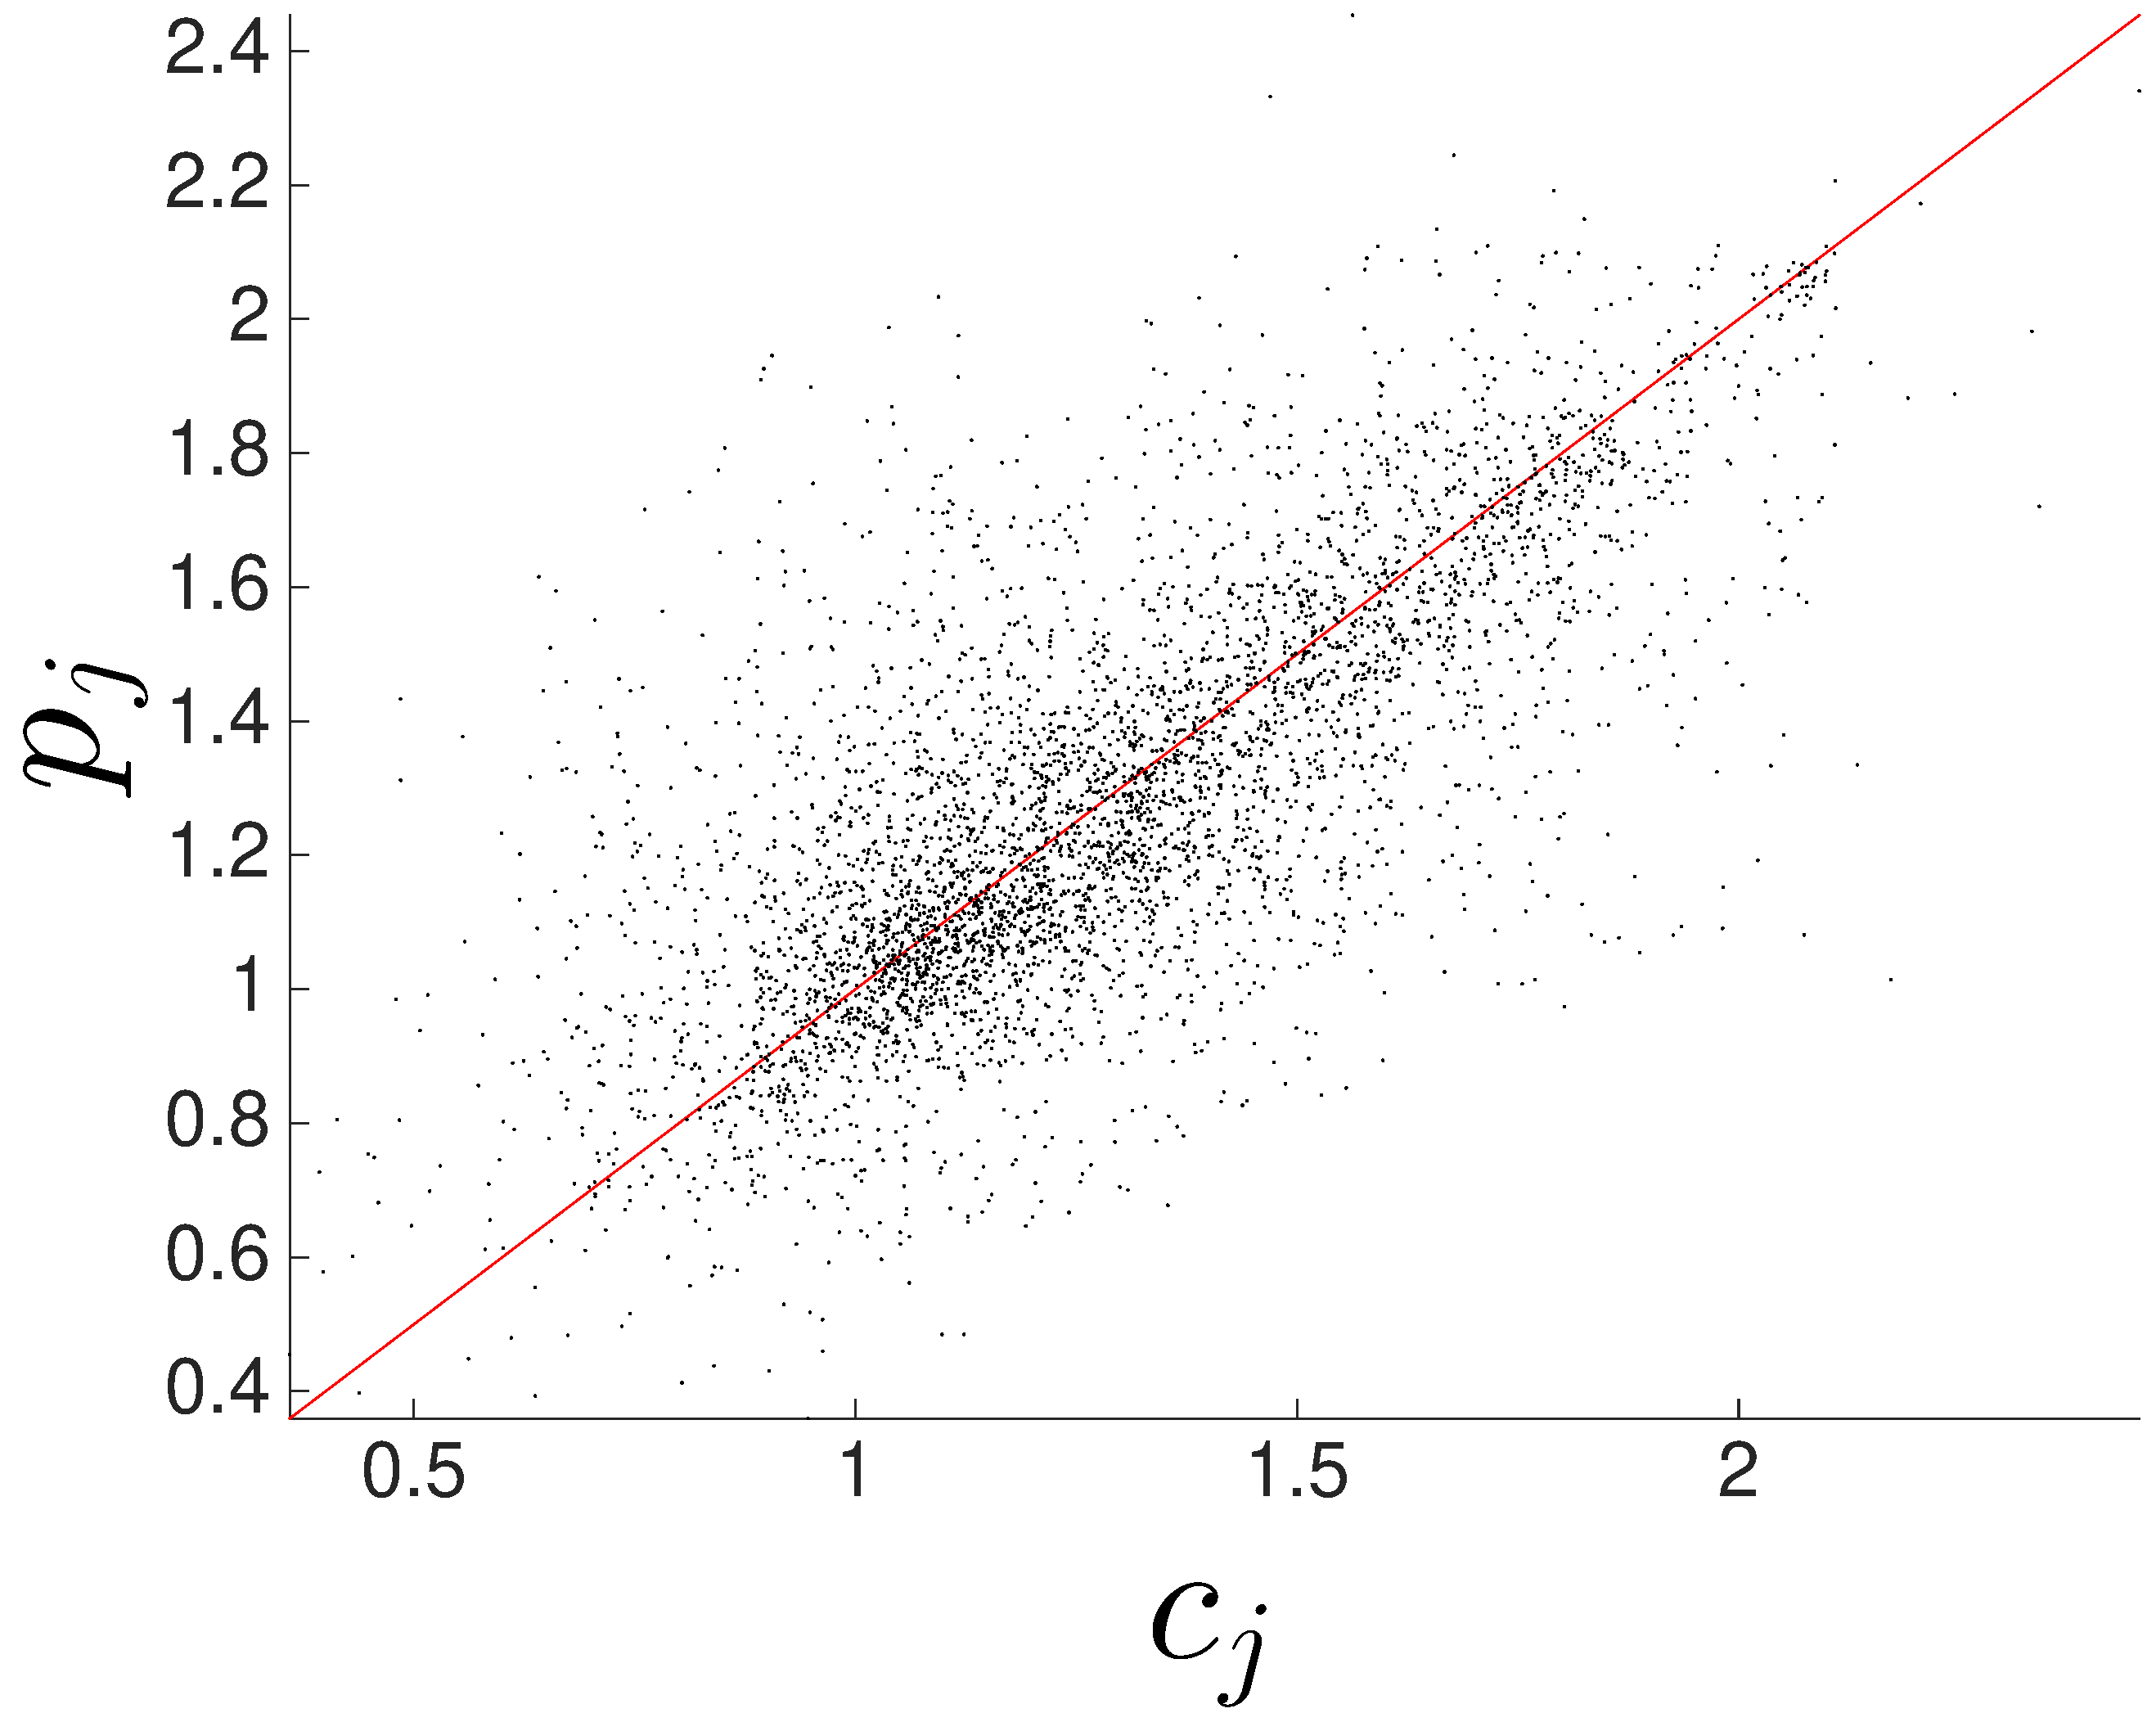
\includegraphics[width=\columnwidth]{figs/gccRWForecast}
%    \caption{\gcc\\ random walk }
%    \label{fig:gccRW}
%  \end{subfigure}%
%     \begin{subfigure}{0.6\columnwidth}
%    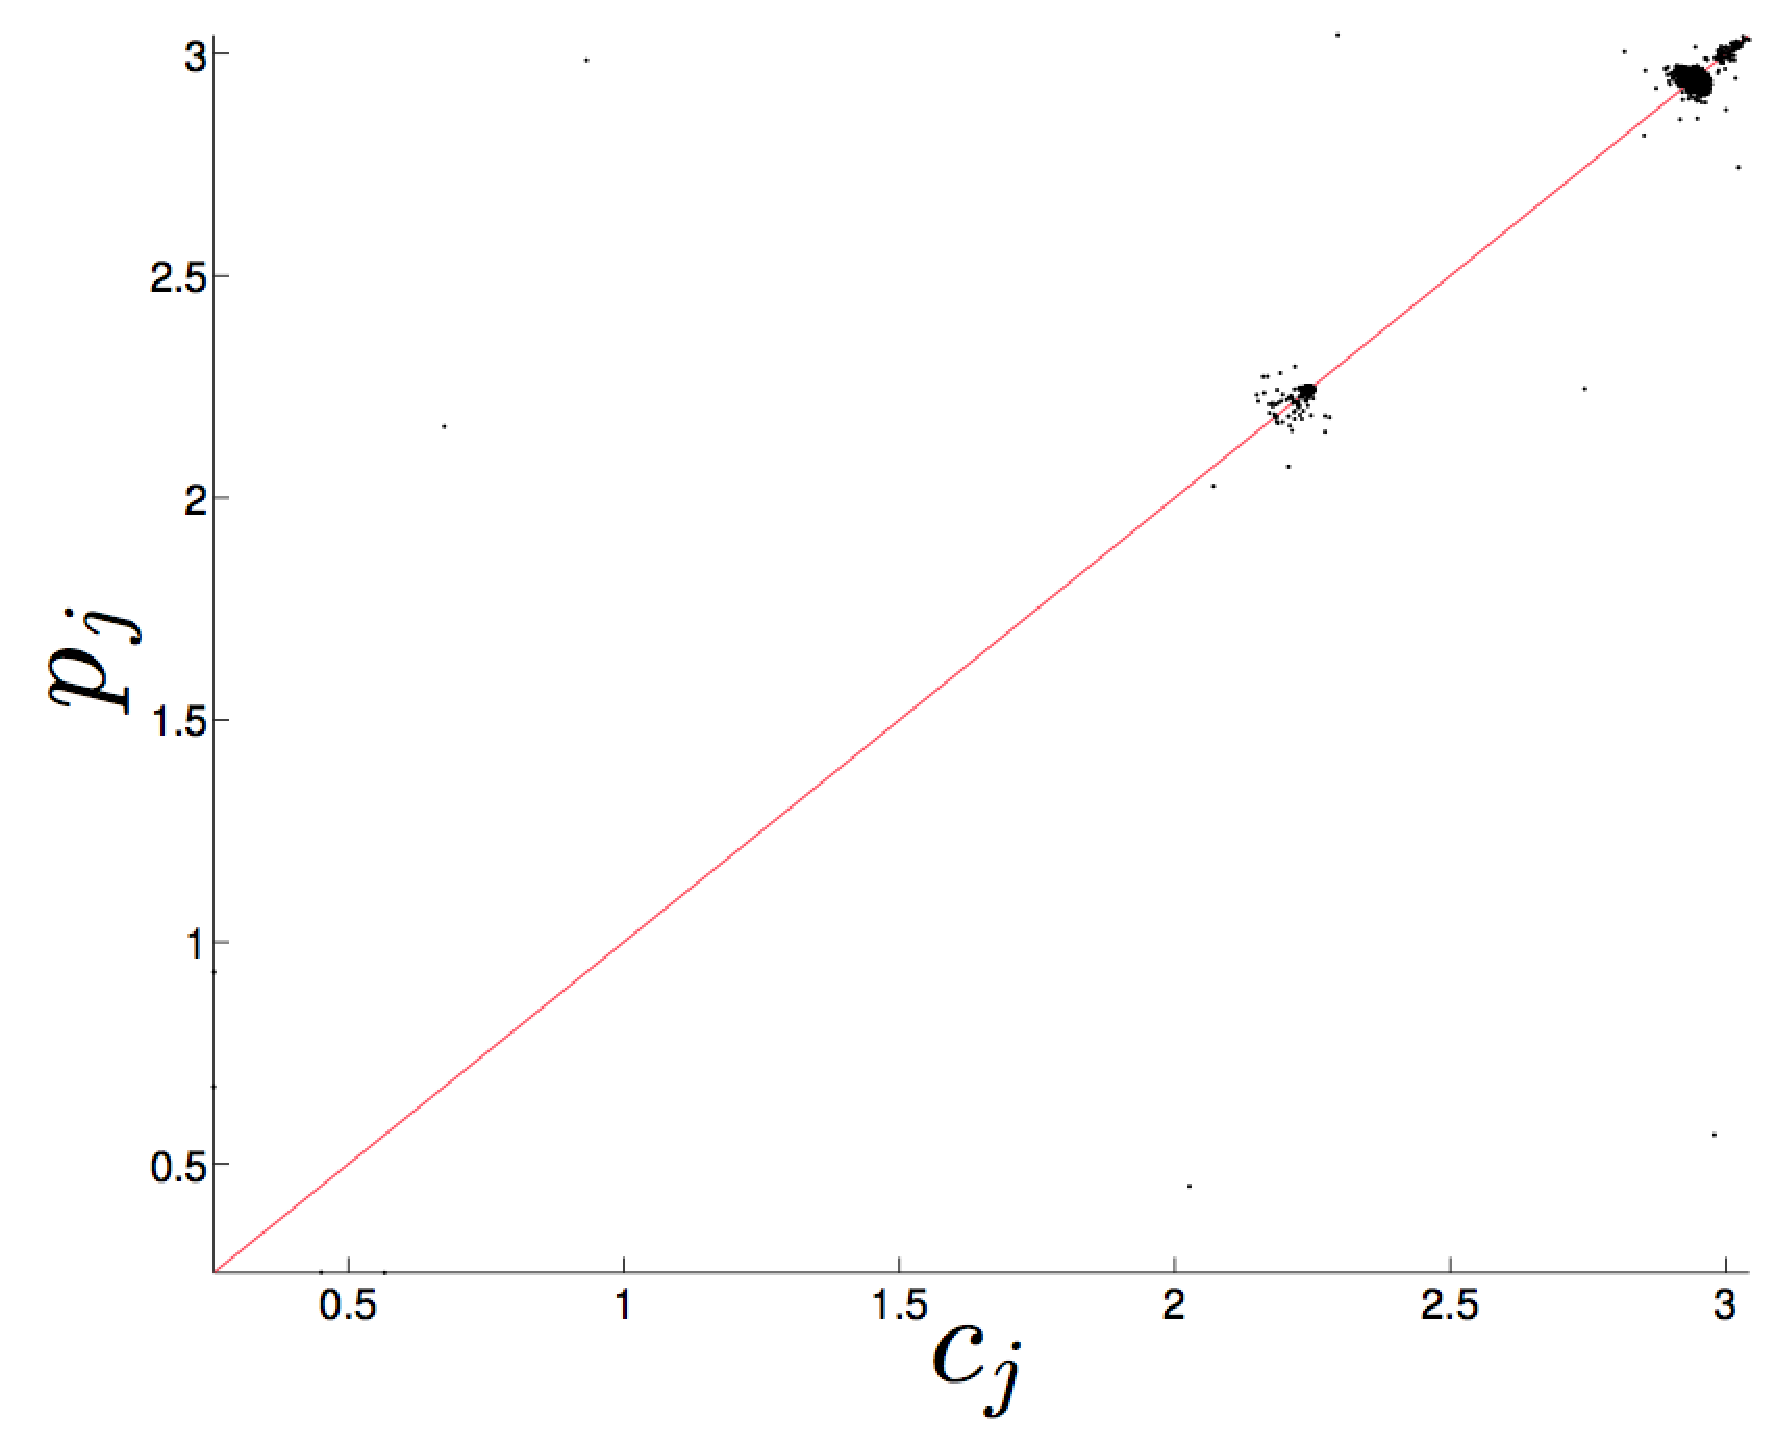
\includegraphics[width=\columnwidth]{figs/svdfiveRWForecast}
%    \caption{\svdfive\\ random walk}
%    \label{fig:svd5RW}
%  \end{subfigure}%
%  \\
%      \begin{subfigure}{0.6\columnwidth}
%    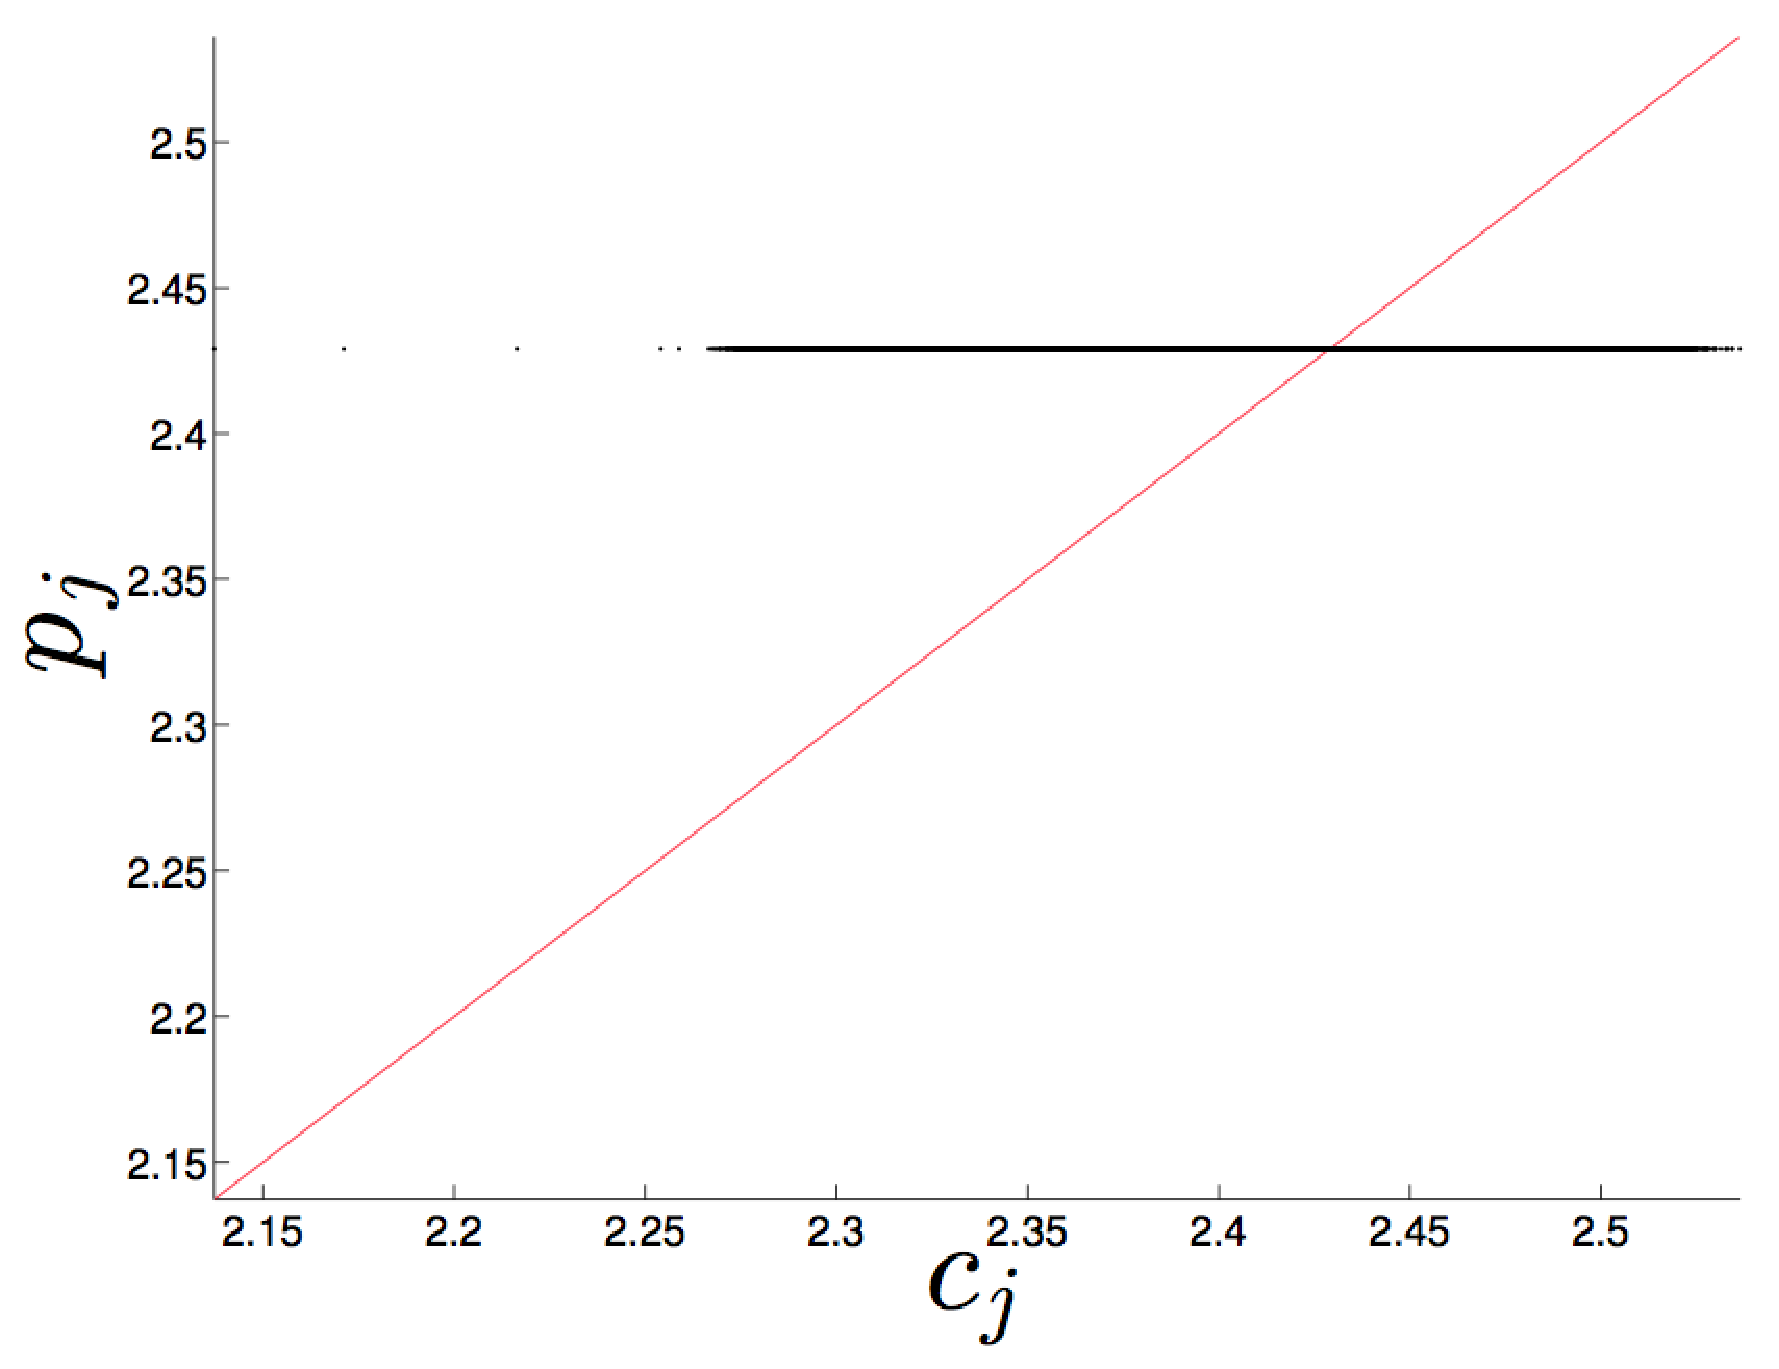
\includegraphics[width=\columnwidth]{figs/colMeanForecast}
%    \caption{\col\\ na\"ive }
%    \label{fig:colMEAN}
%  \end{subfigure}%
%   \begin{subfigure}{0.6\columnwidth}
%    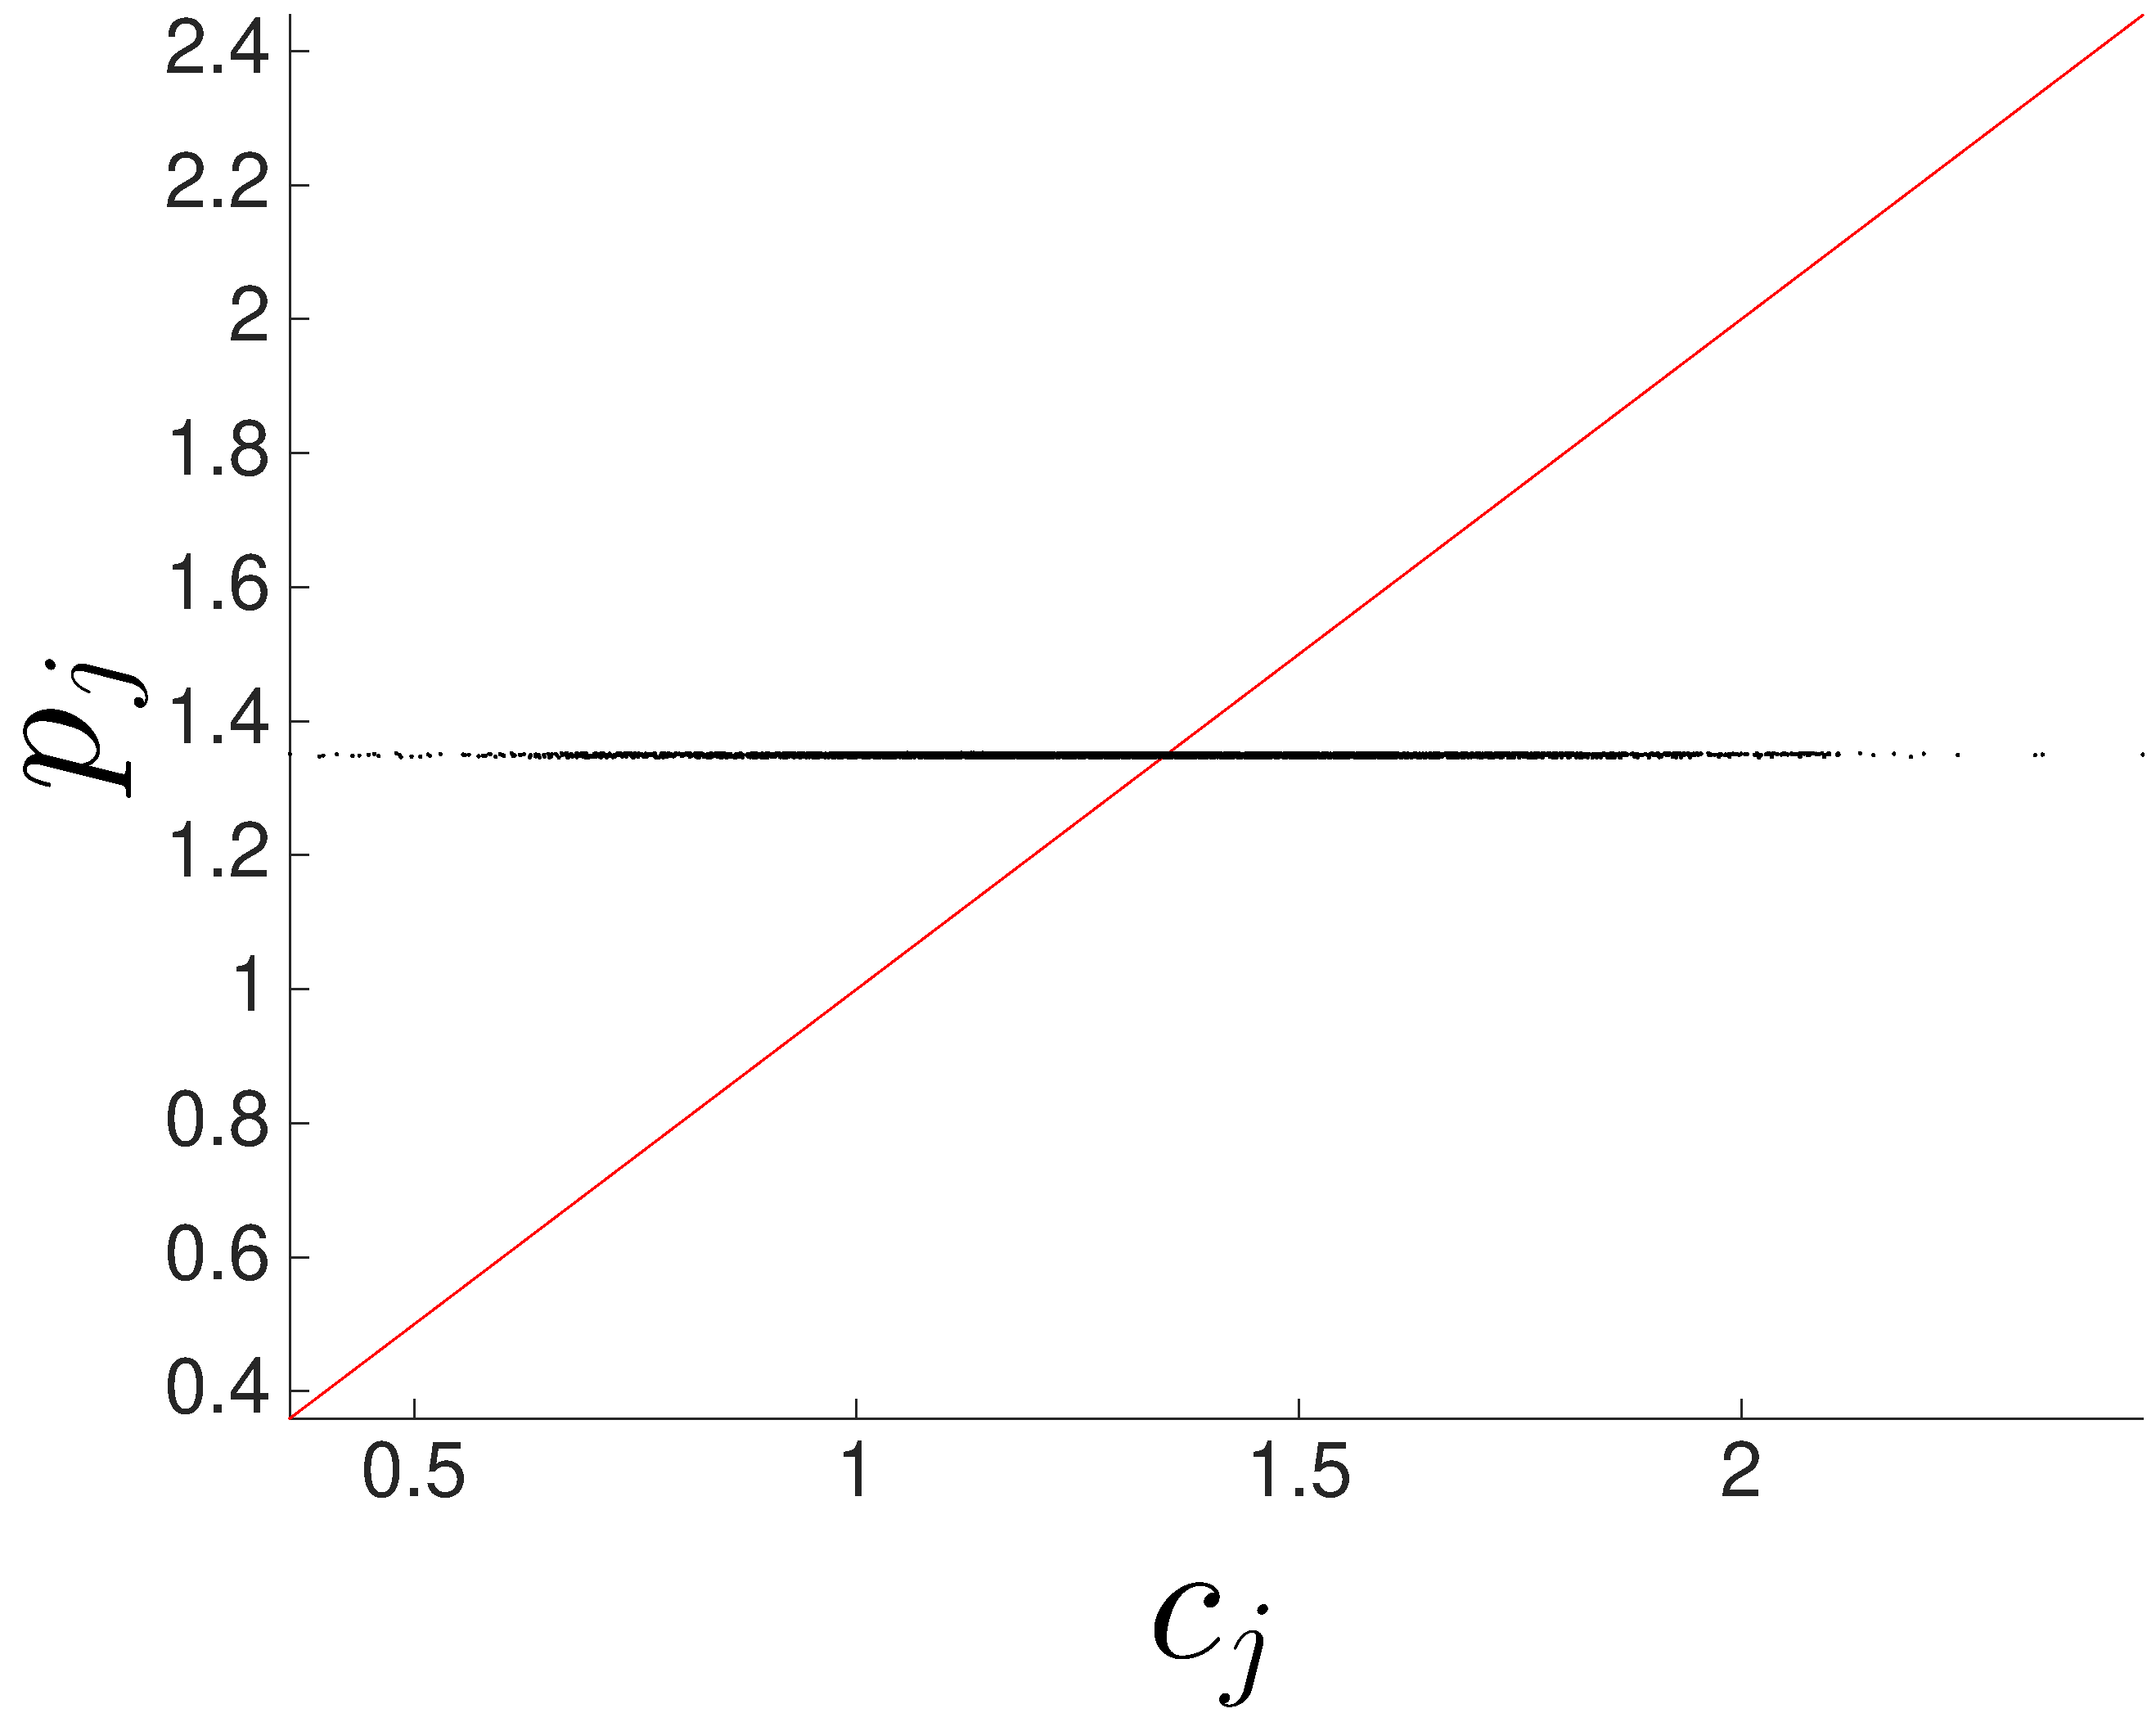
\includegraphics[width=\columnwidth]{figs/gccMeanForecast}
%    \caption{\gcc\\ na\"ive }
%    \label{fig:gccMEAN}
%  \end{subfigure}%
%     \begin{subfigure}{0.6\columnwidth}
%    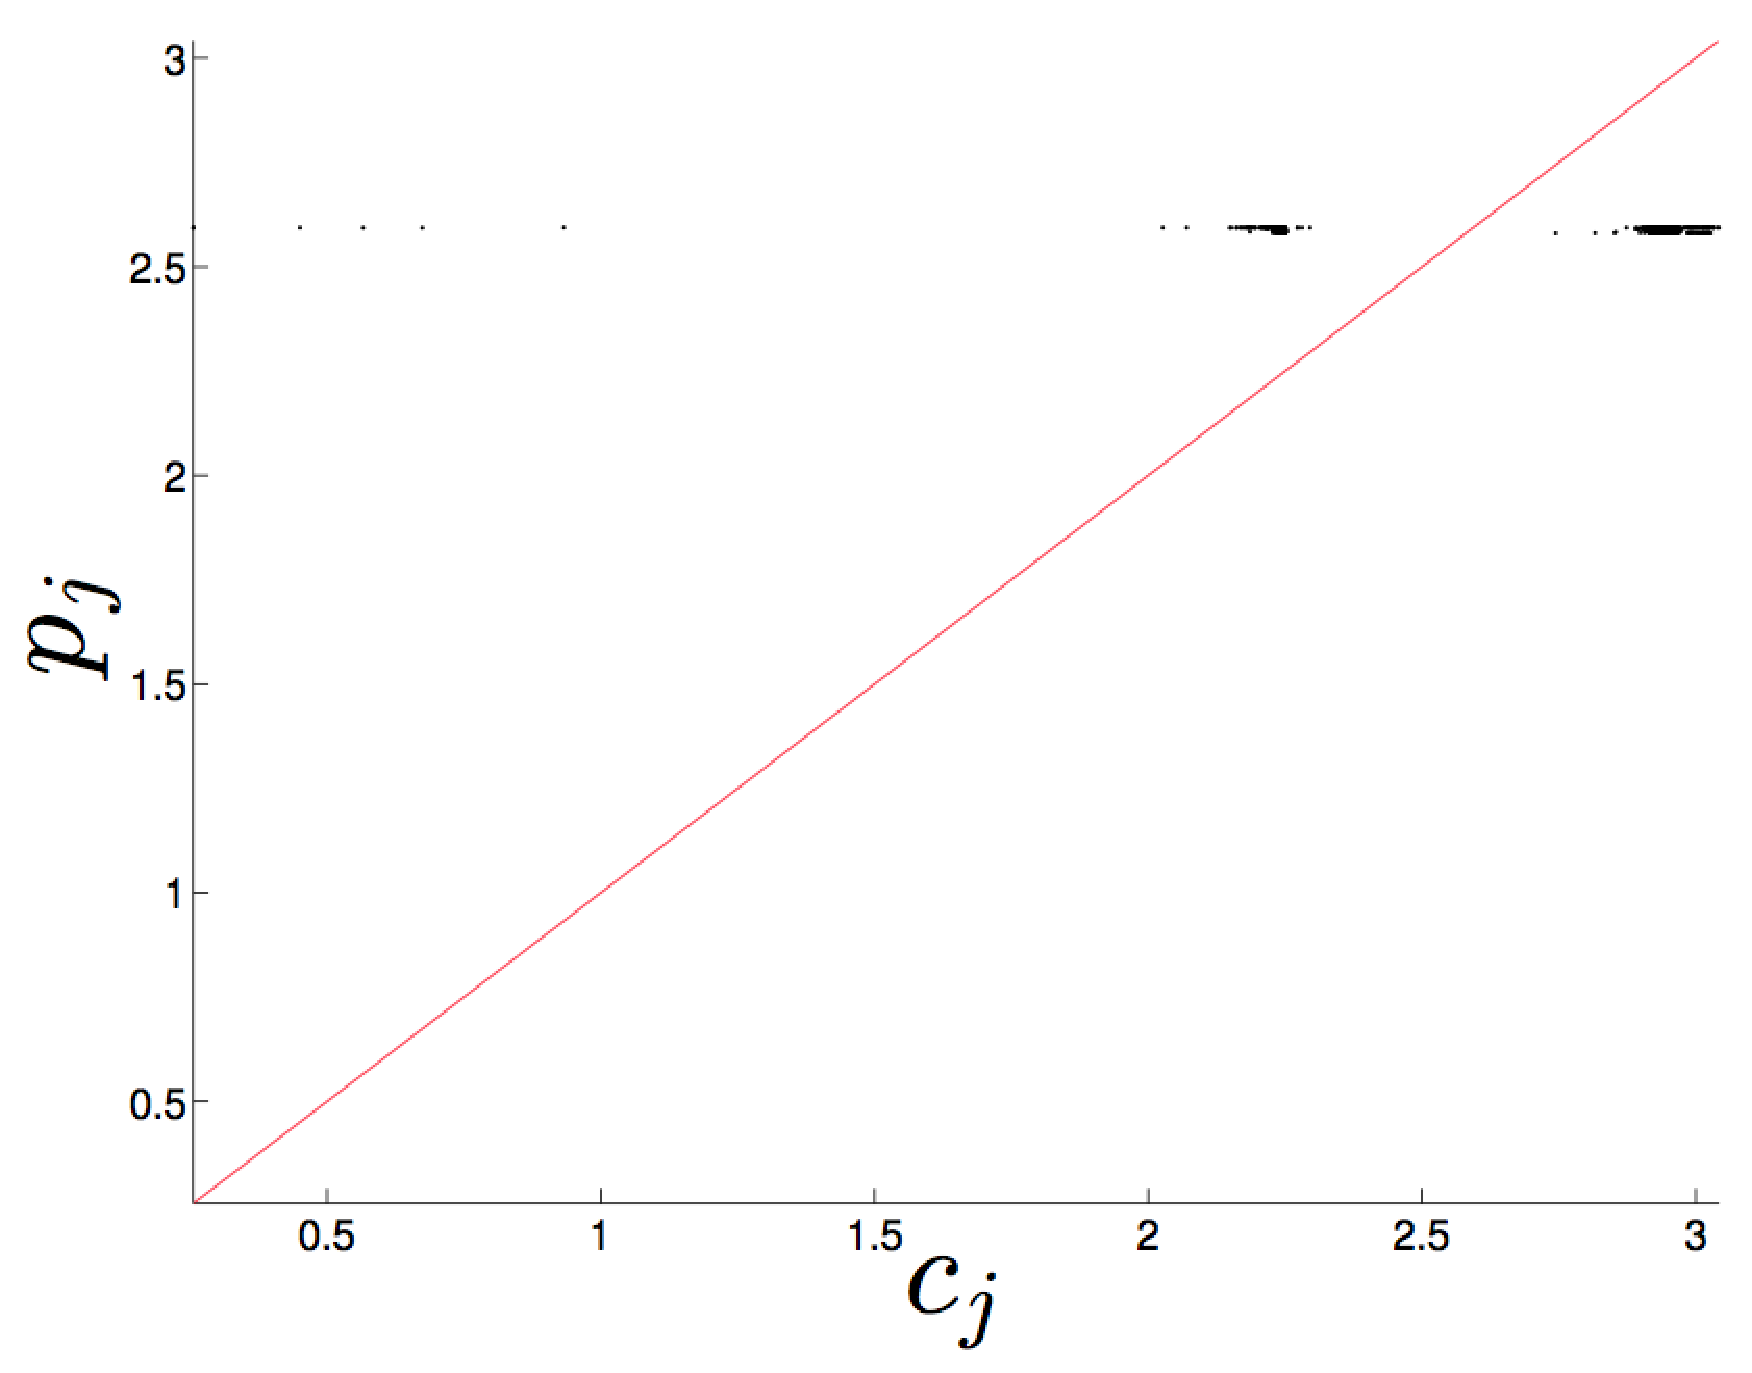
\includegraphics[width=\columnwidth]{figs/svdfiveMeanForecast}
%    \caption{\svdfive\\ na\"ive }
%    \label{fig:svd5MEAN}
%  \end{subfigure}%
%  \\
%    \begin{subfigure}{0.6\columnwidth}
%    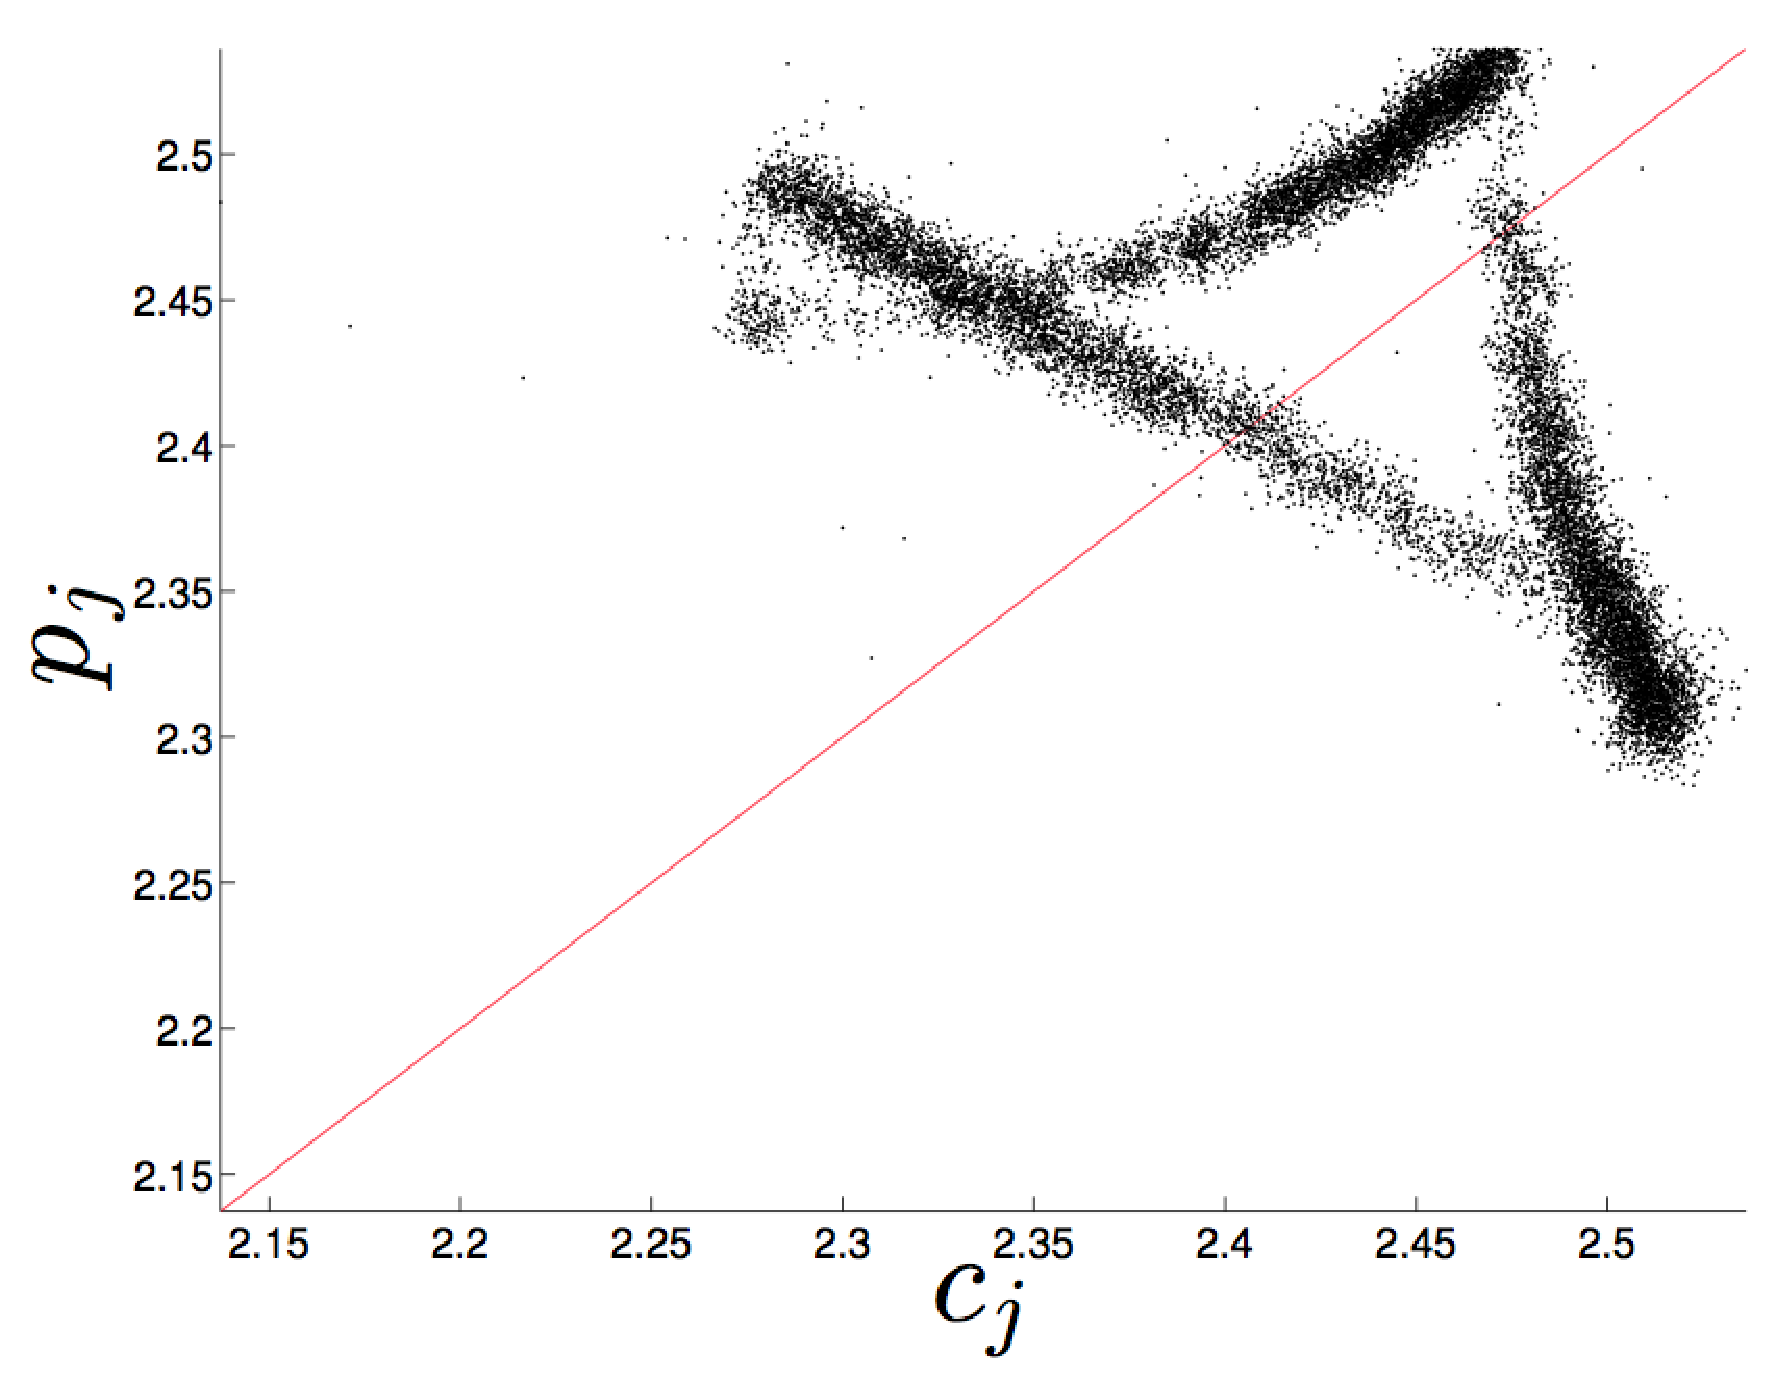
\includegraphics[width=\columnwidth]{figs/colARIMAForecast}
%    \caption{\col \\ \arima}
%    \label{fig:colARIMA}
%  \end{subfigure}
%  \begin{subfigure}{0.6\columnwidth}
%    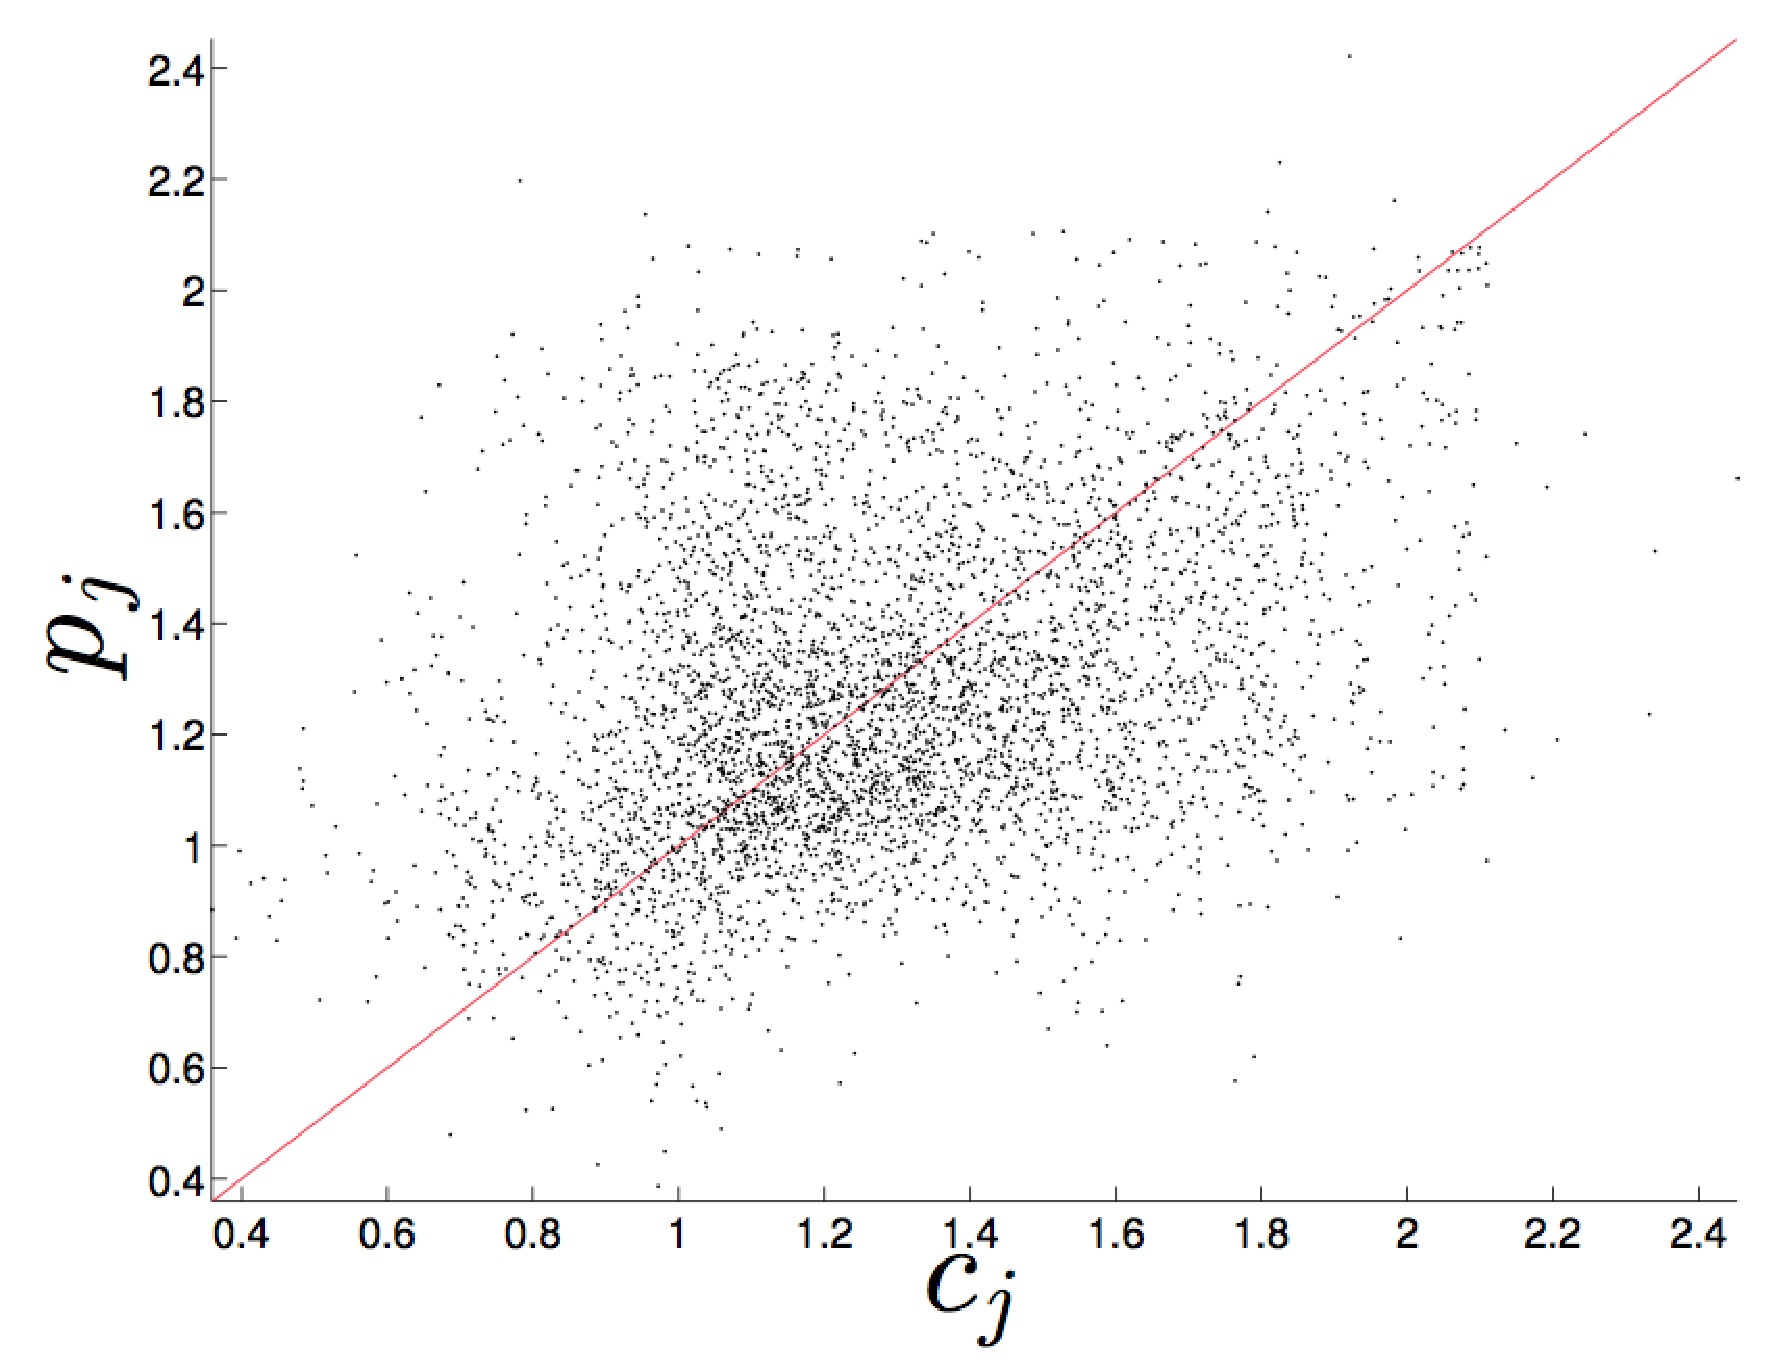
\includegraphics[width=\columnwidth]{figs/gccARIMAForecast}
%    \caption{\gcc \\ \arima }
%    \label{fig:gccARIMA}
%  \end{subfigure}%
%  \begin{subfigure}{0.6\columnwidth}
%    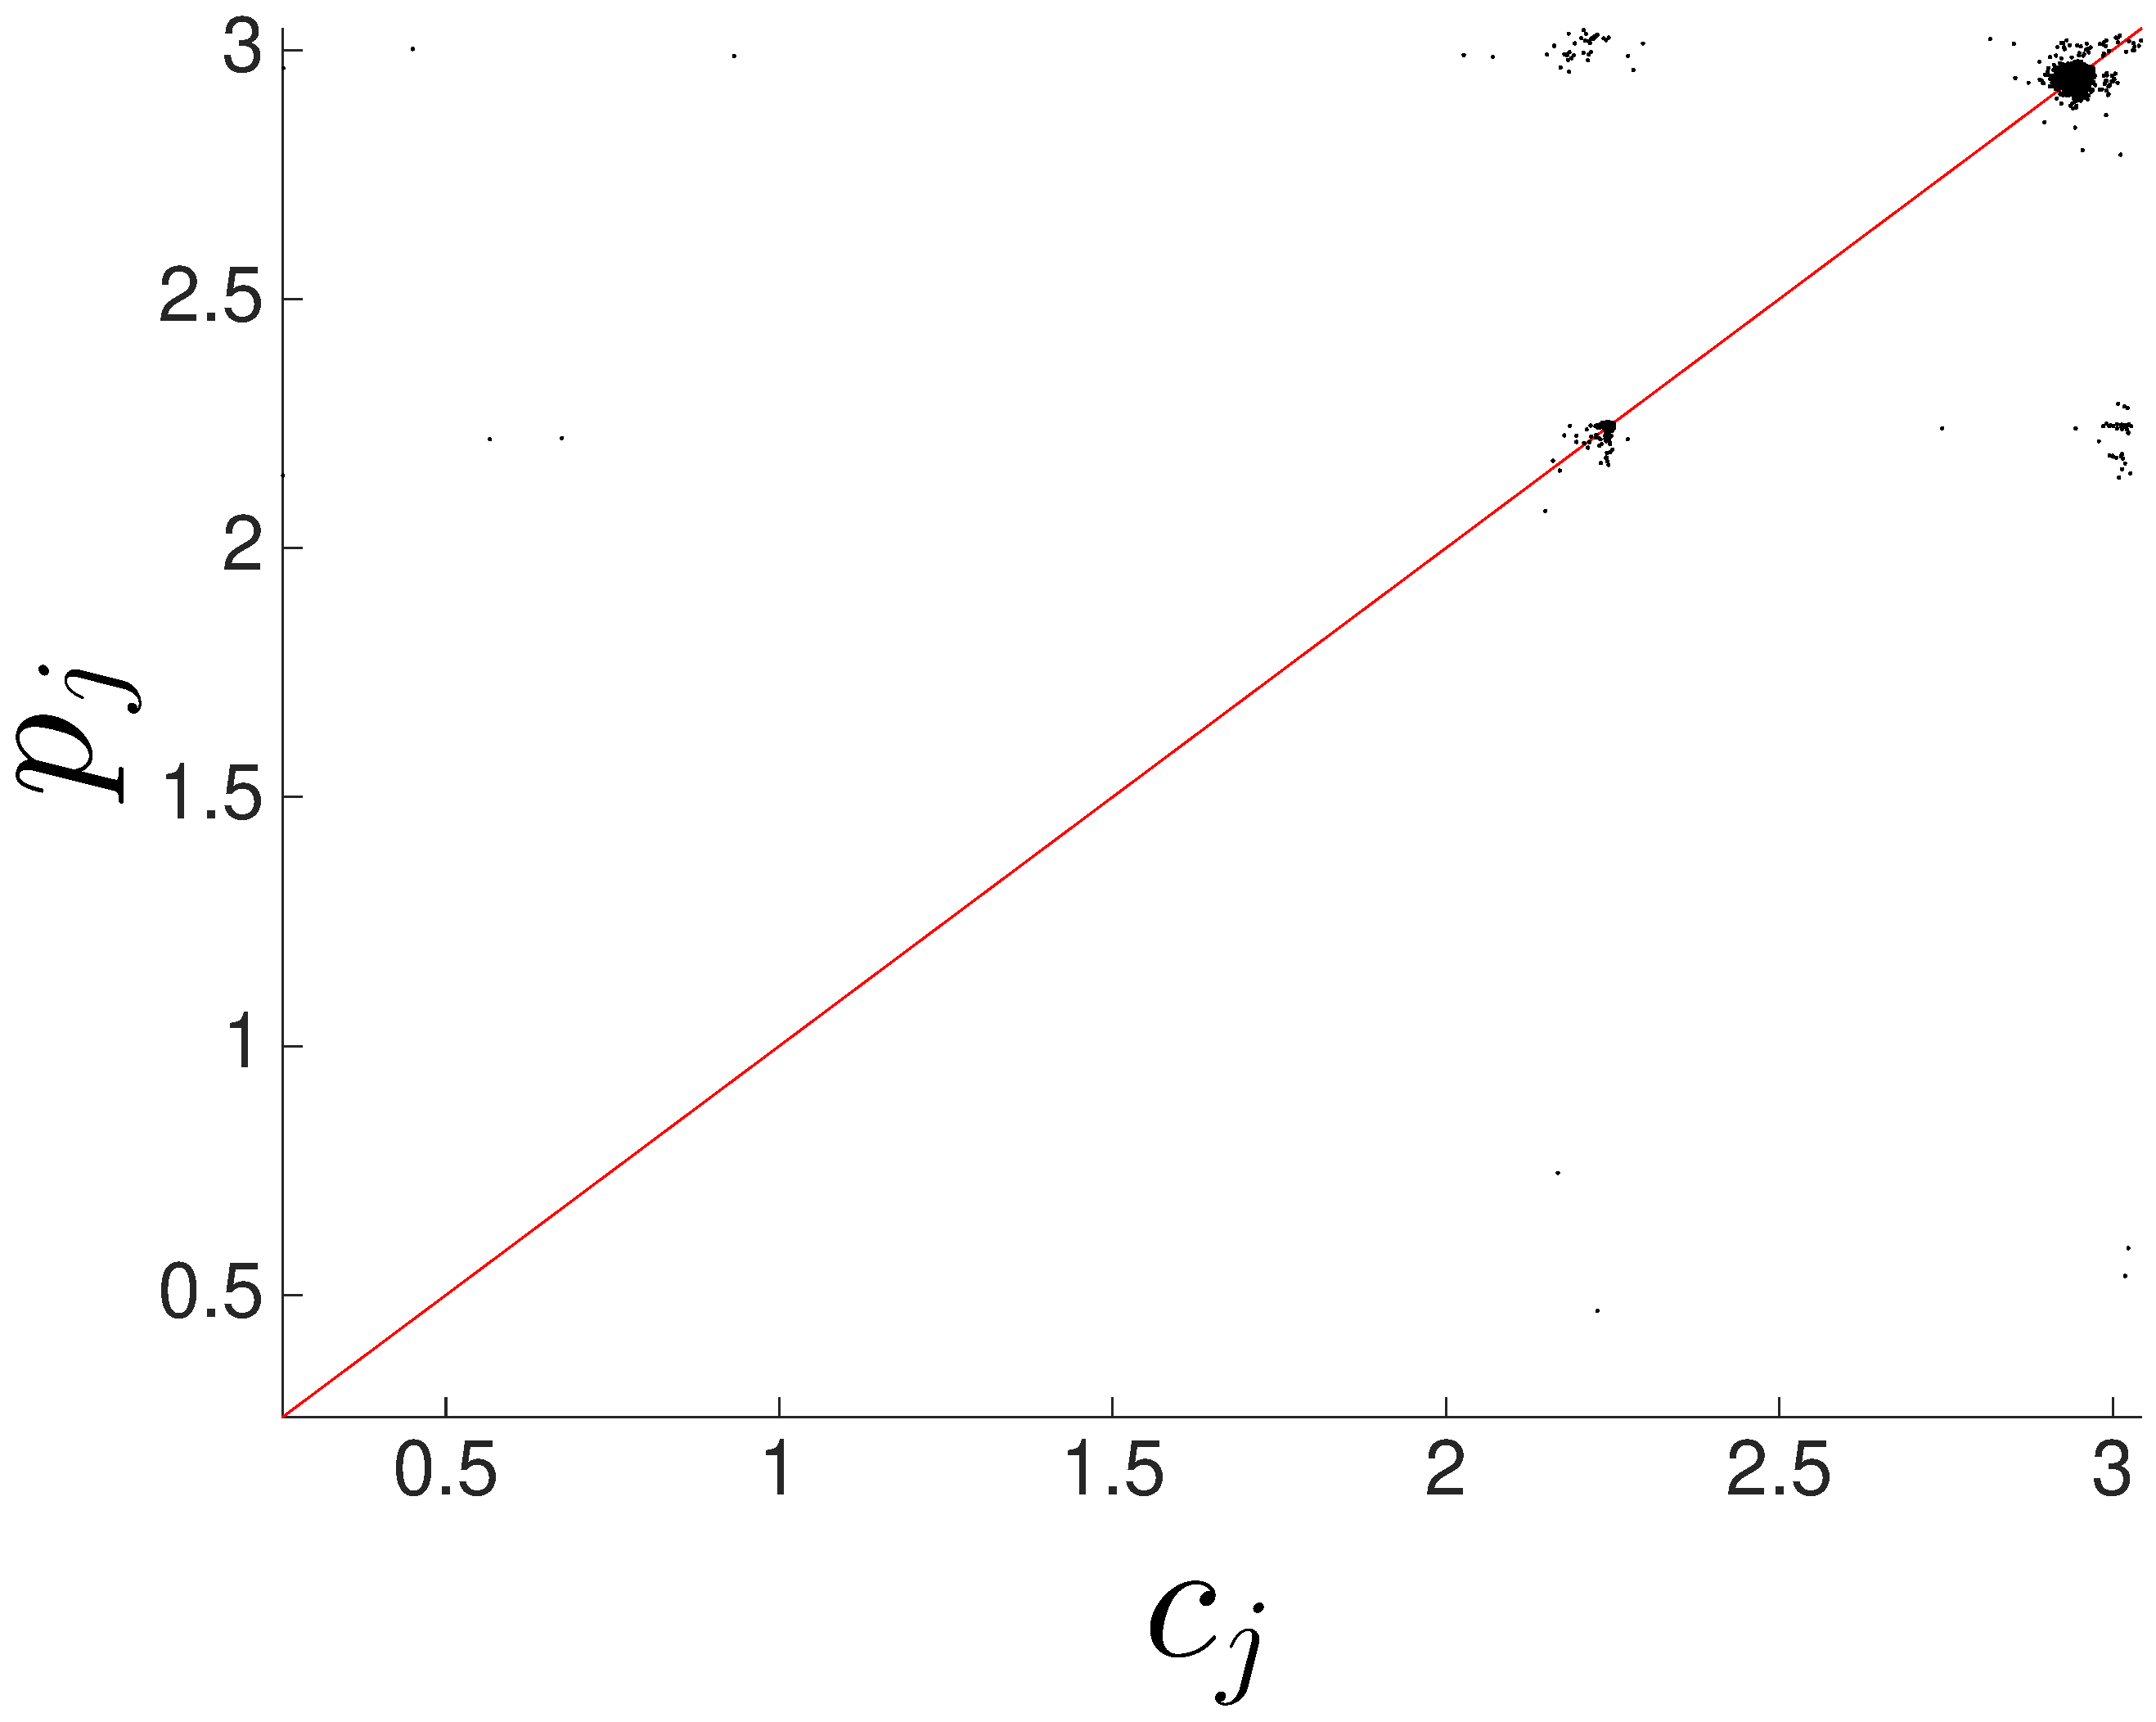
\includegraphics[width=\columnwidth]{figs/svdfiveARIMAForecast}
%    \caption{\svdfive \\ \arima }
%    \label{fig:svd5ARIMA}
%  \end{subfigure}%
%  \\
%
%      \begin{subfigure}{0.6\columnwidth}
%    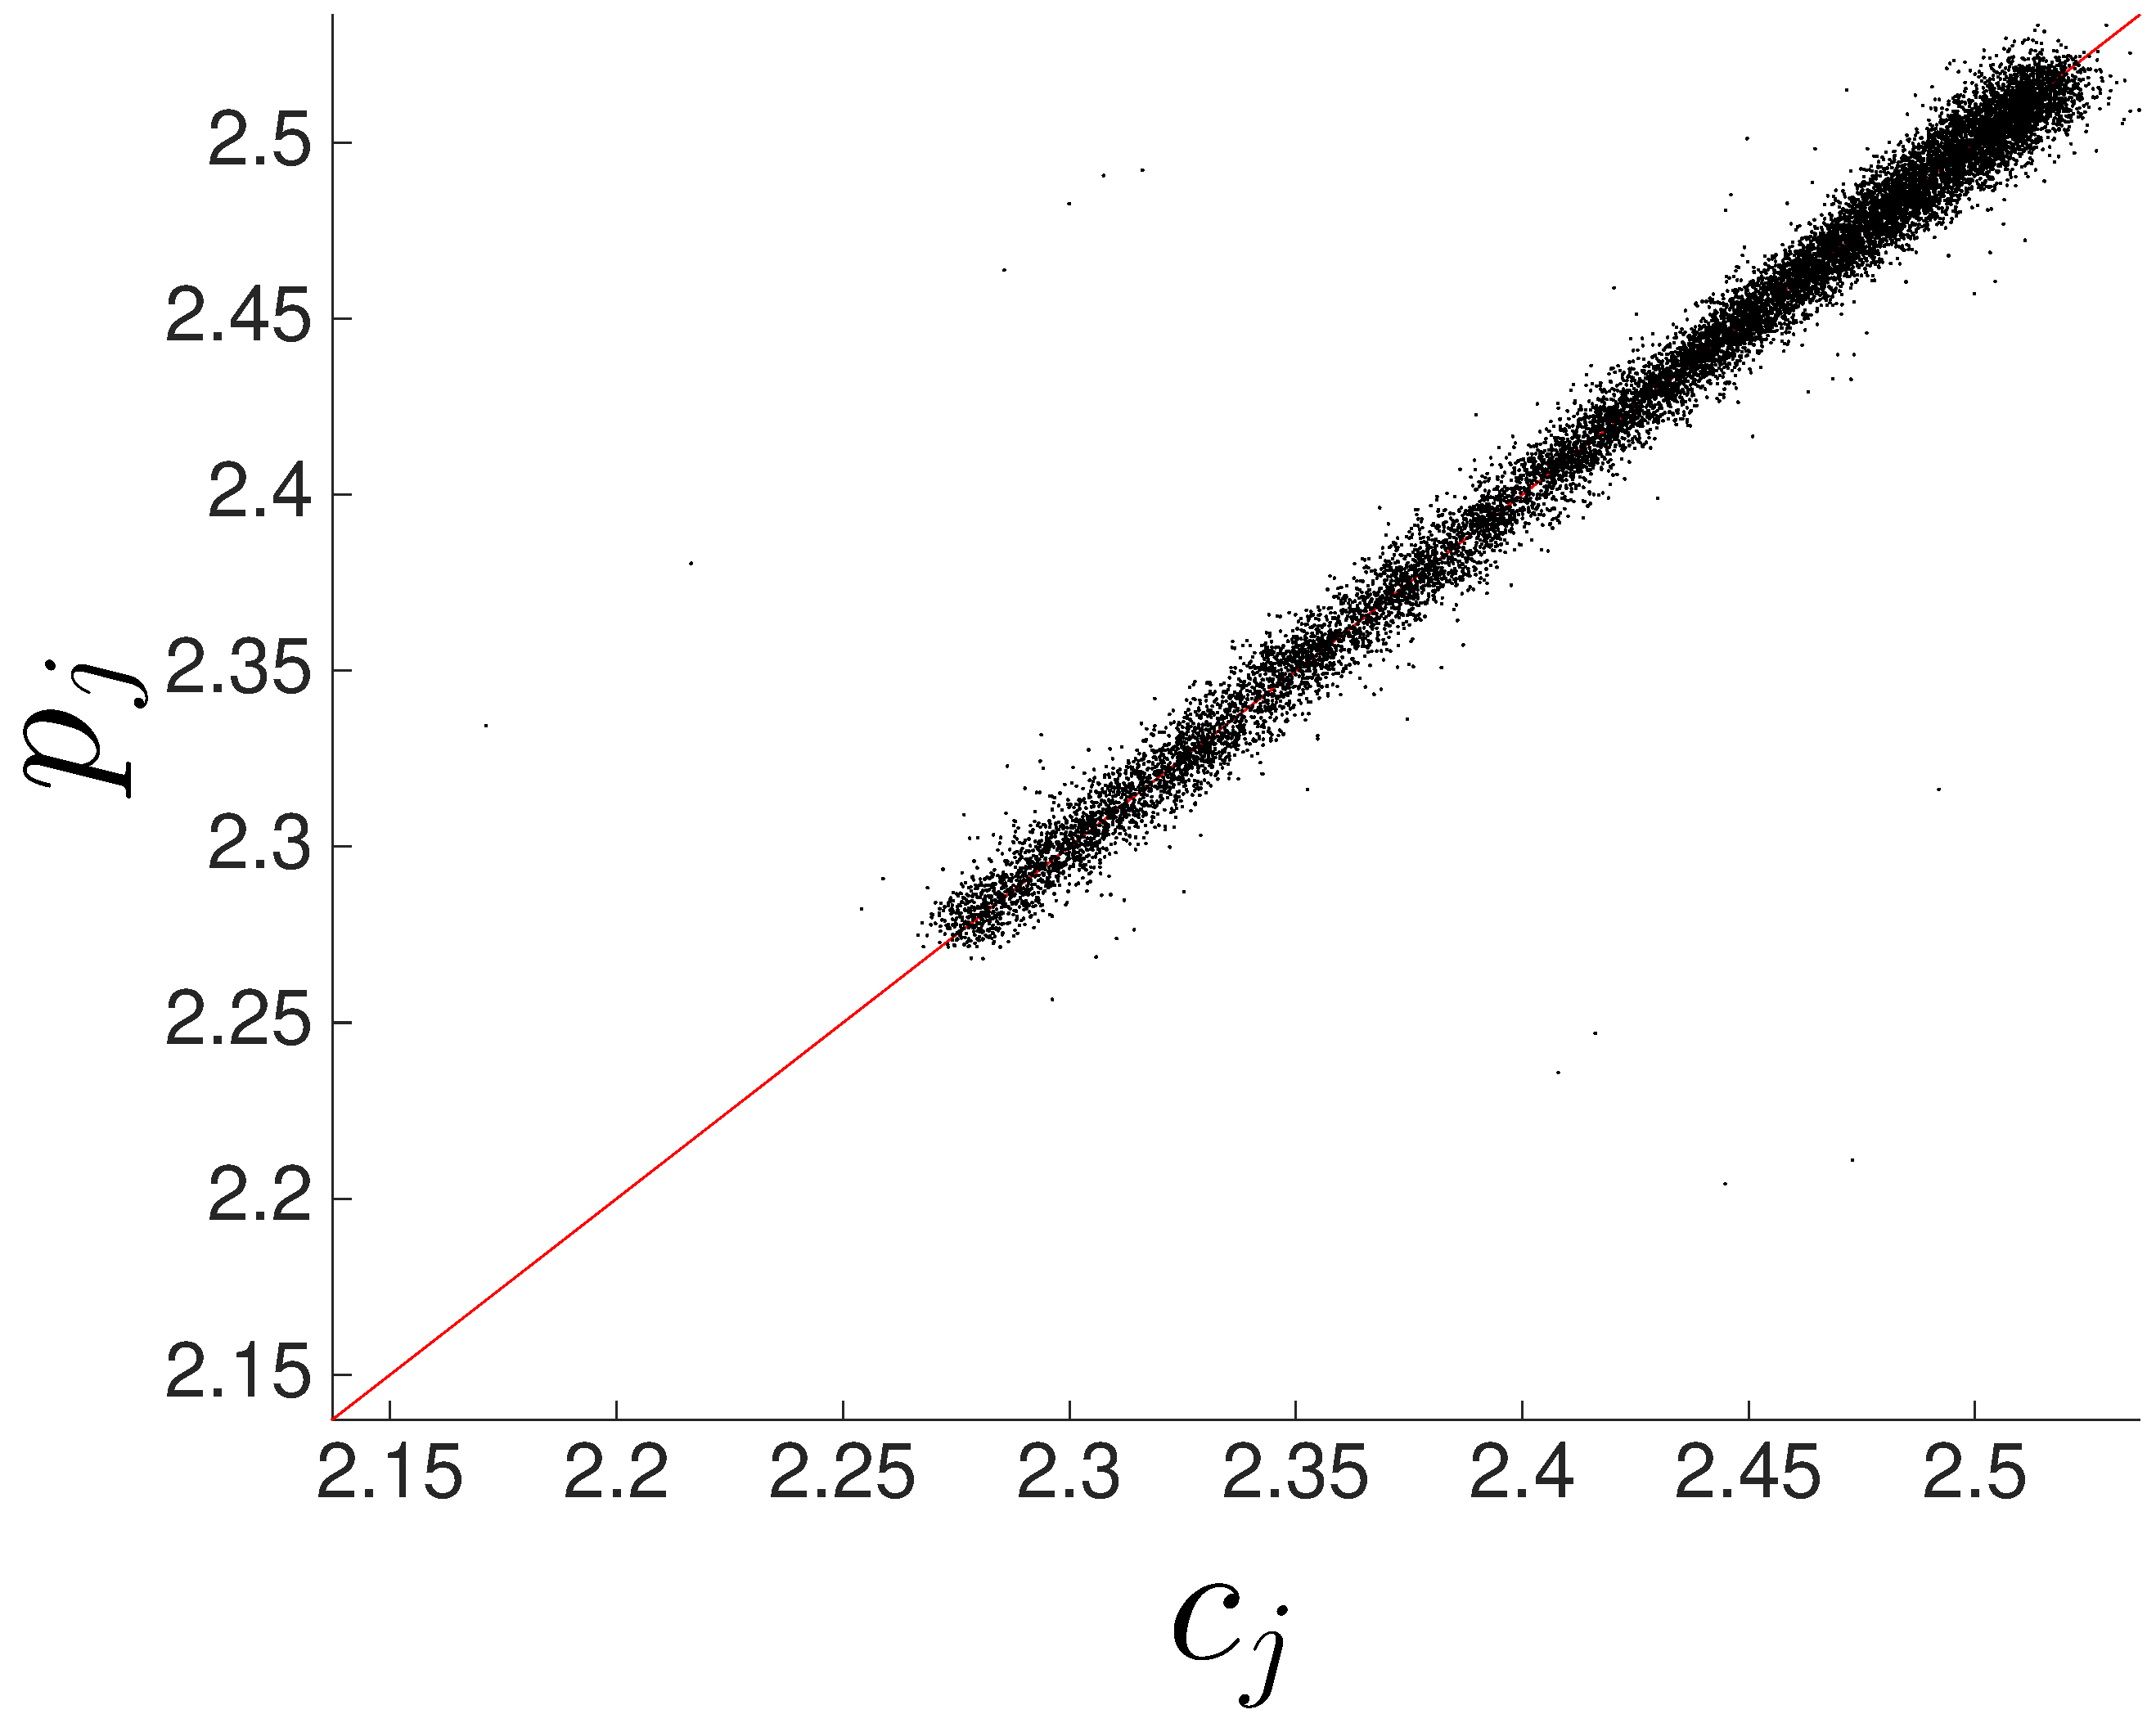
\includegraphics[width=\columnwidth]{figs/colLMAForecast}
%    \caption{\col \\ LMA}
%    \label{fig:colLMA}
%  \end{subfigure}
%      \begin{subfigure}{0.6\columnwidth}
%    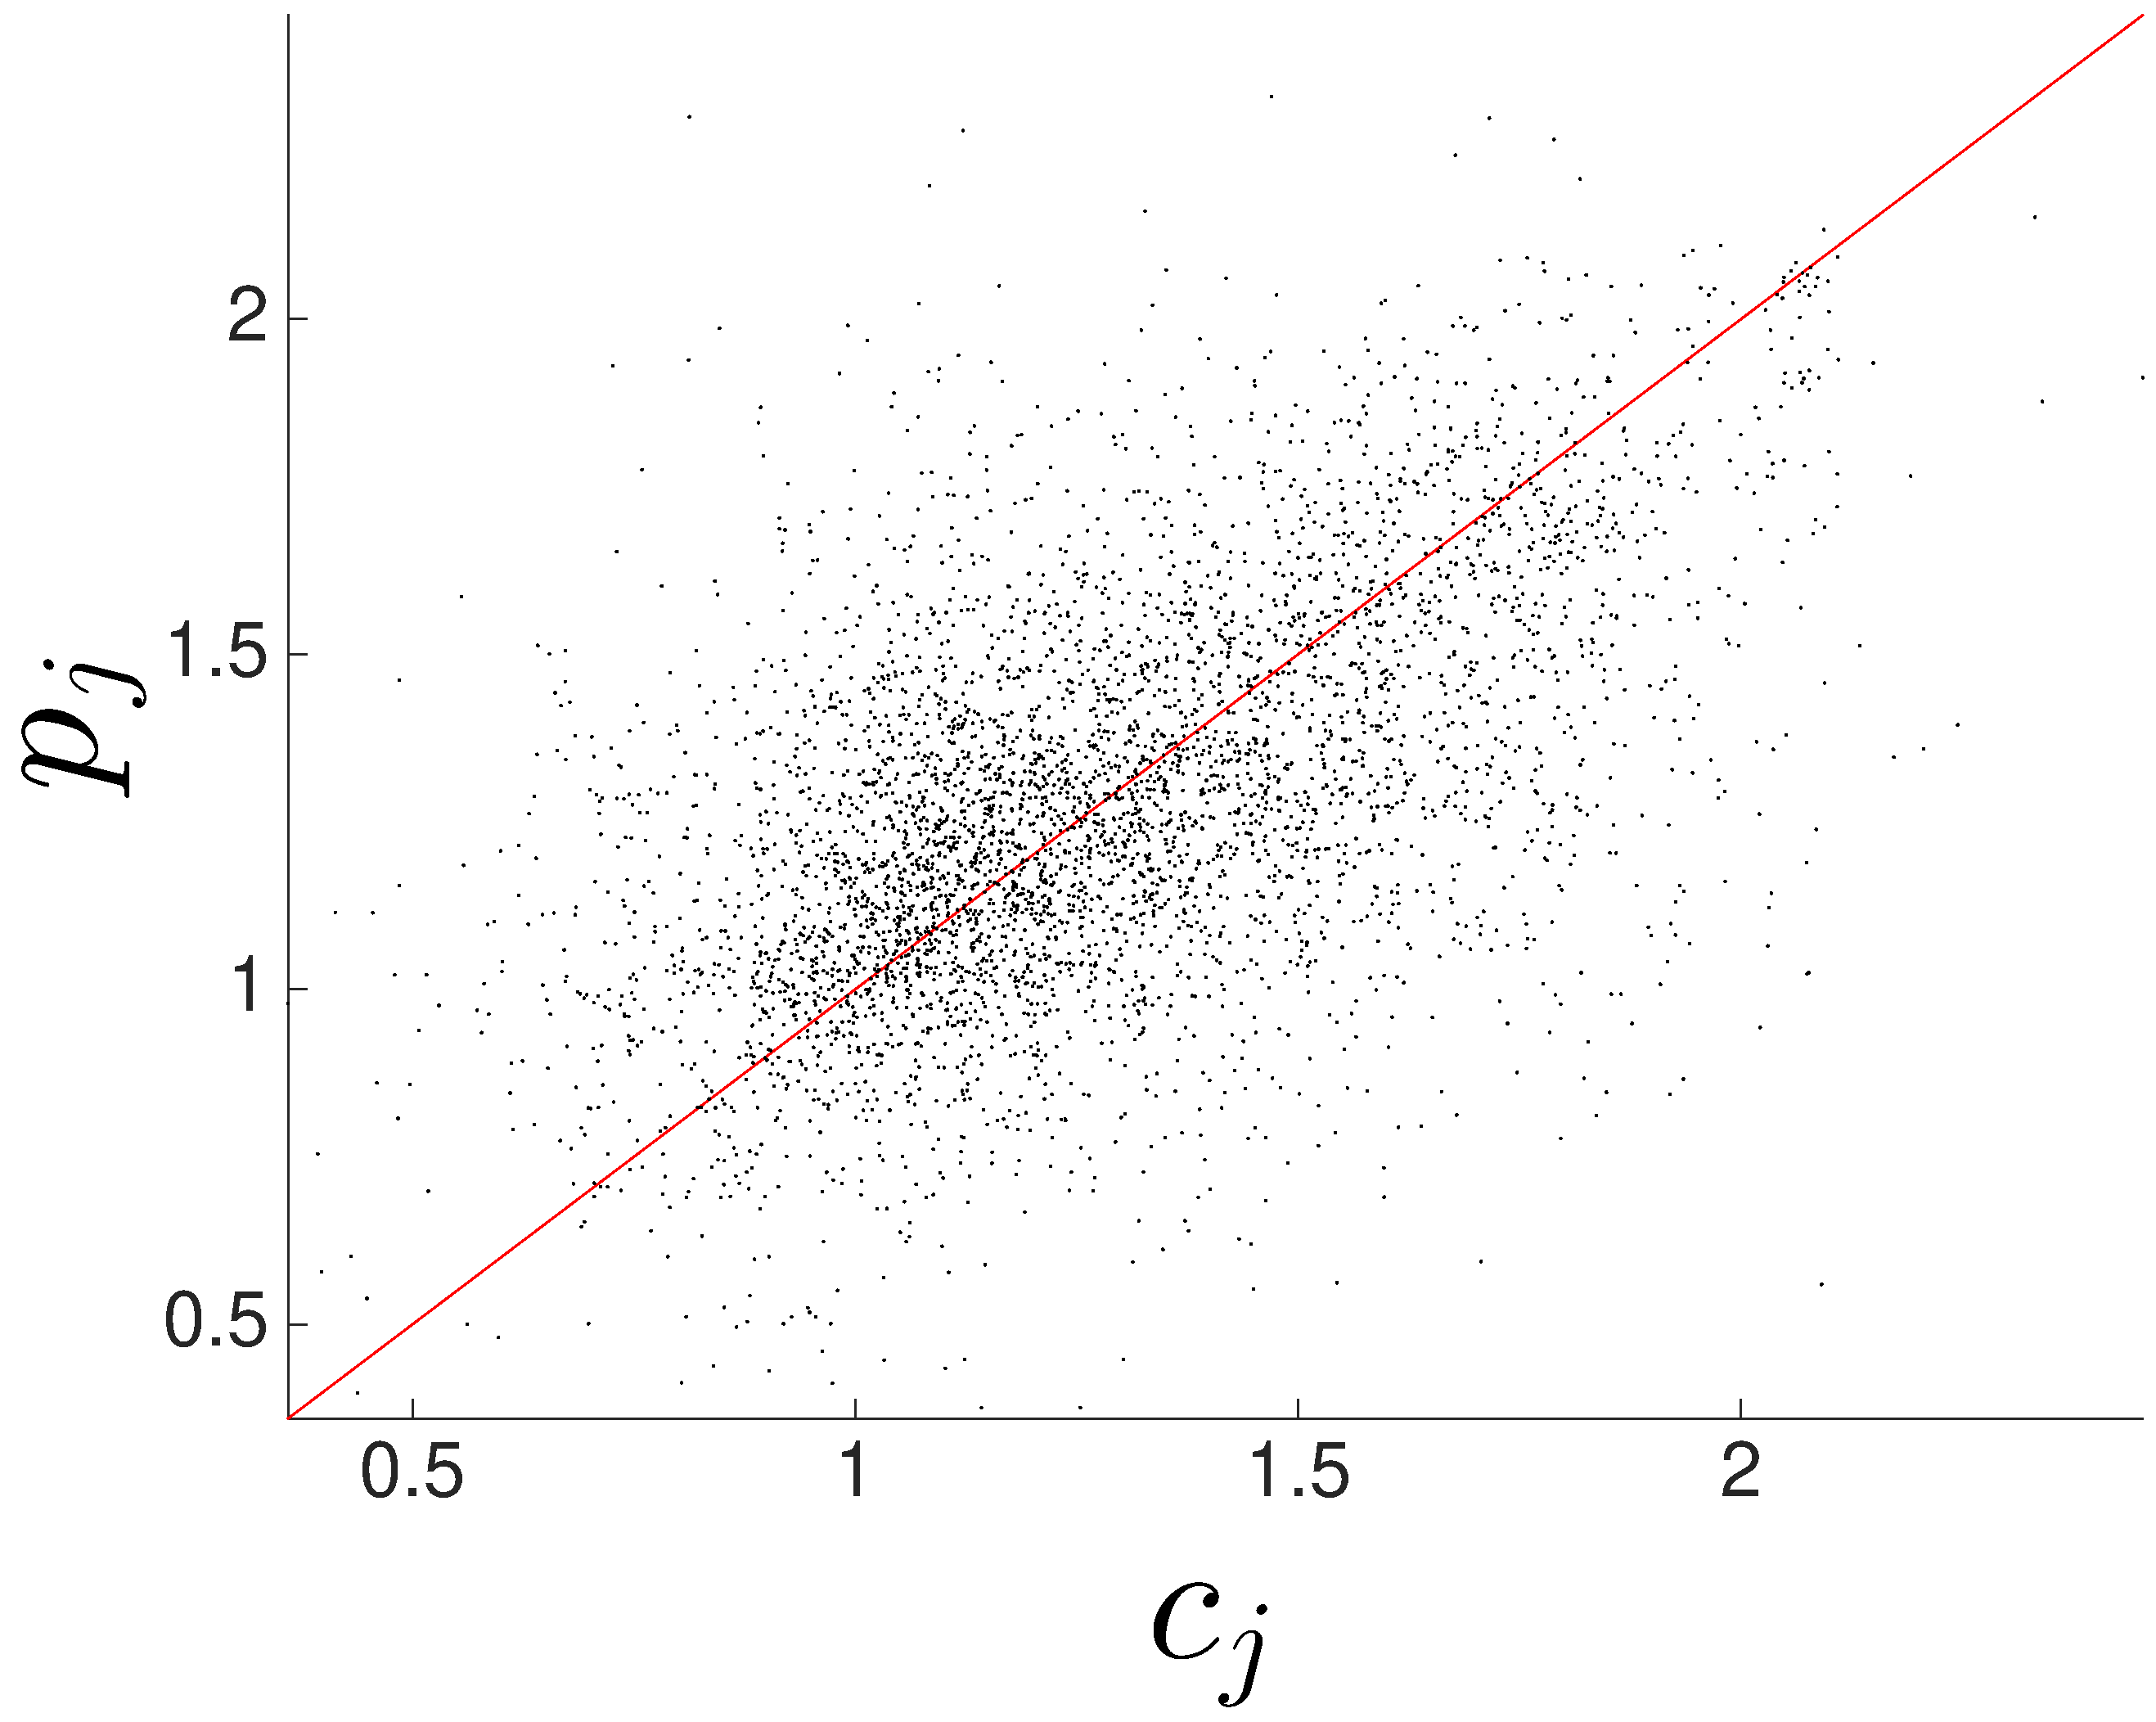
\includegraphics[width=\columnwidth]{figs/gccLMAForecast}
%    \caption{\gcc \\ LMA}
%    \label{fig:gccLMA}
%  \end{subfigure}
%        \begin{subfigure}{0.6\columnwidth}
%    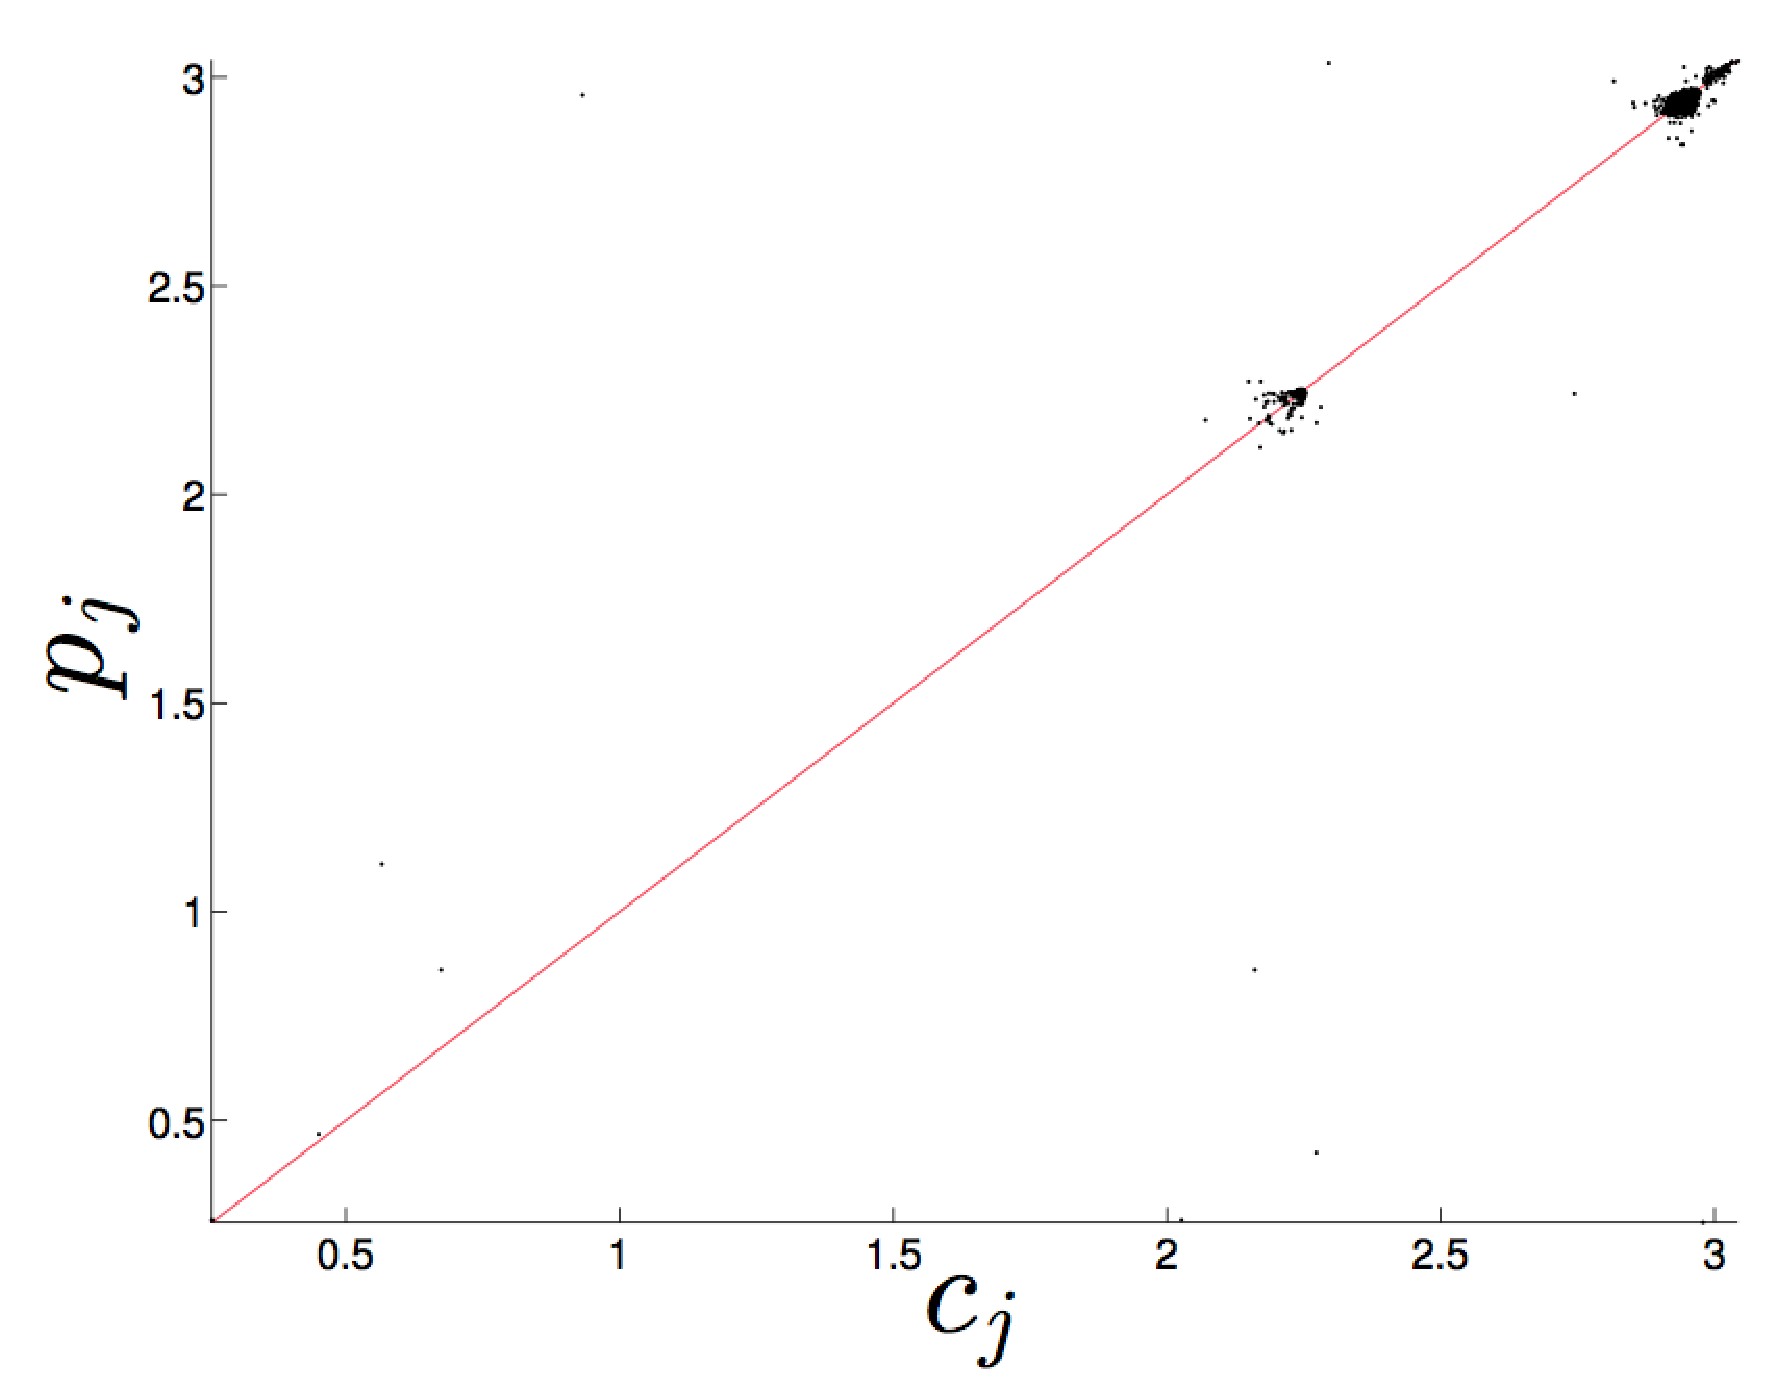
\includegraphics[width=\columnwidth]{figs/svdfiveLMAForecast}
%    \caption{\svdfive \\ LMA}
%    \label{fig:svd5LMA}
%  \end{subfigure}
%  %\begin{subfigure}{0.5\textwidth}
%  %  \includegraphics[width=1.0\textwidth]{LMA_vs_ARIMA}
%   \caption{Predicted ($p_j$) versus true values ($c_j$) for
%     forecasts of \col, \gcc, and \svdfive and all four prediction strategies.
%% On this type of plot, a perfect prediction lies exactly on the
%% diagonal.
%%
%%
%}
%\label{fig:forecast-example}
%  %\end{subfigure}
%\end{figure*}
\newcolumntype{C}{>{\centering\arraybackslash} m{0.6\columnwidth} }
\begin{figure*}
  \renewcommand{\arraystretch}{1.25}
  \begin{tabular}{m{0.1\columnwidth}|CCC}
    & {\large \col} & {\large \gcc} & {\large \svdfive} \\
    & & & \\
            \hline \\
    \rotatebox{90}{\large{random walk}} &
    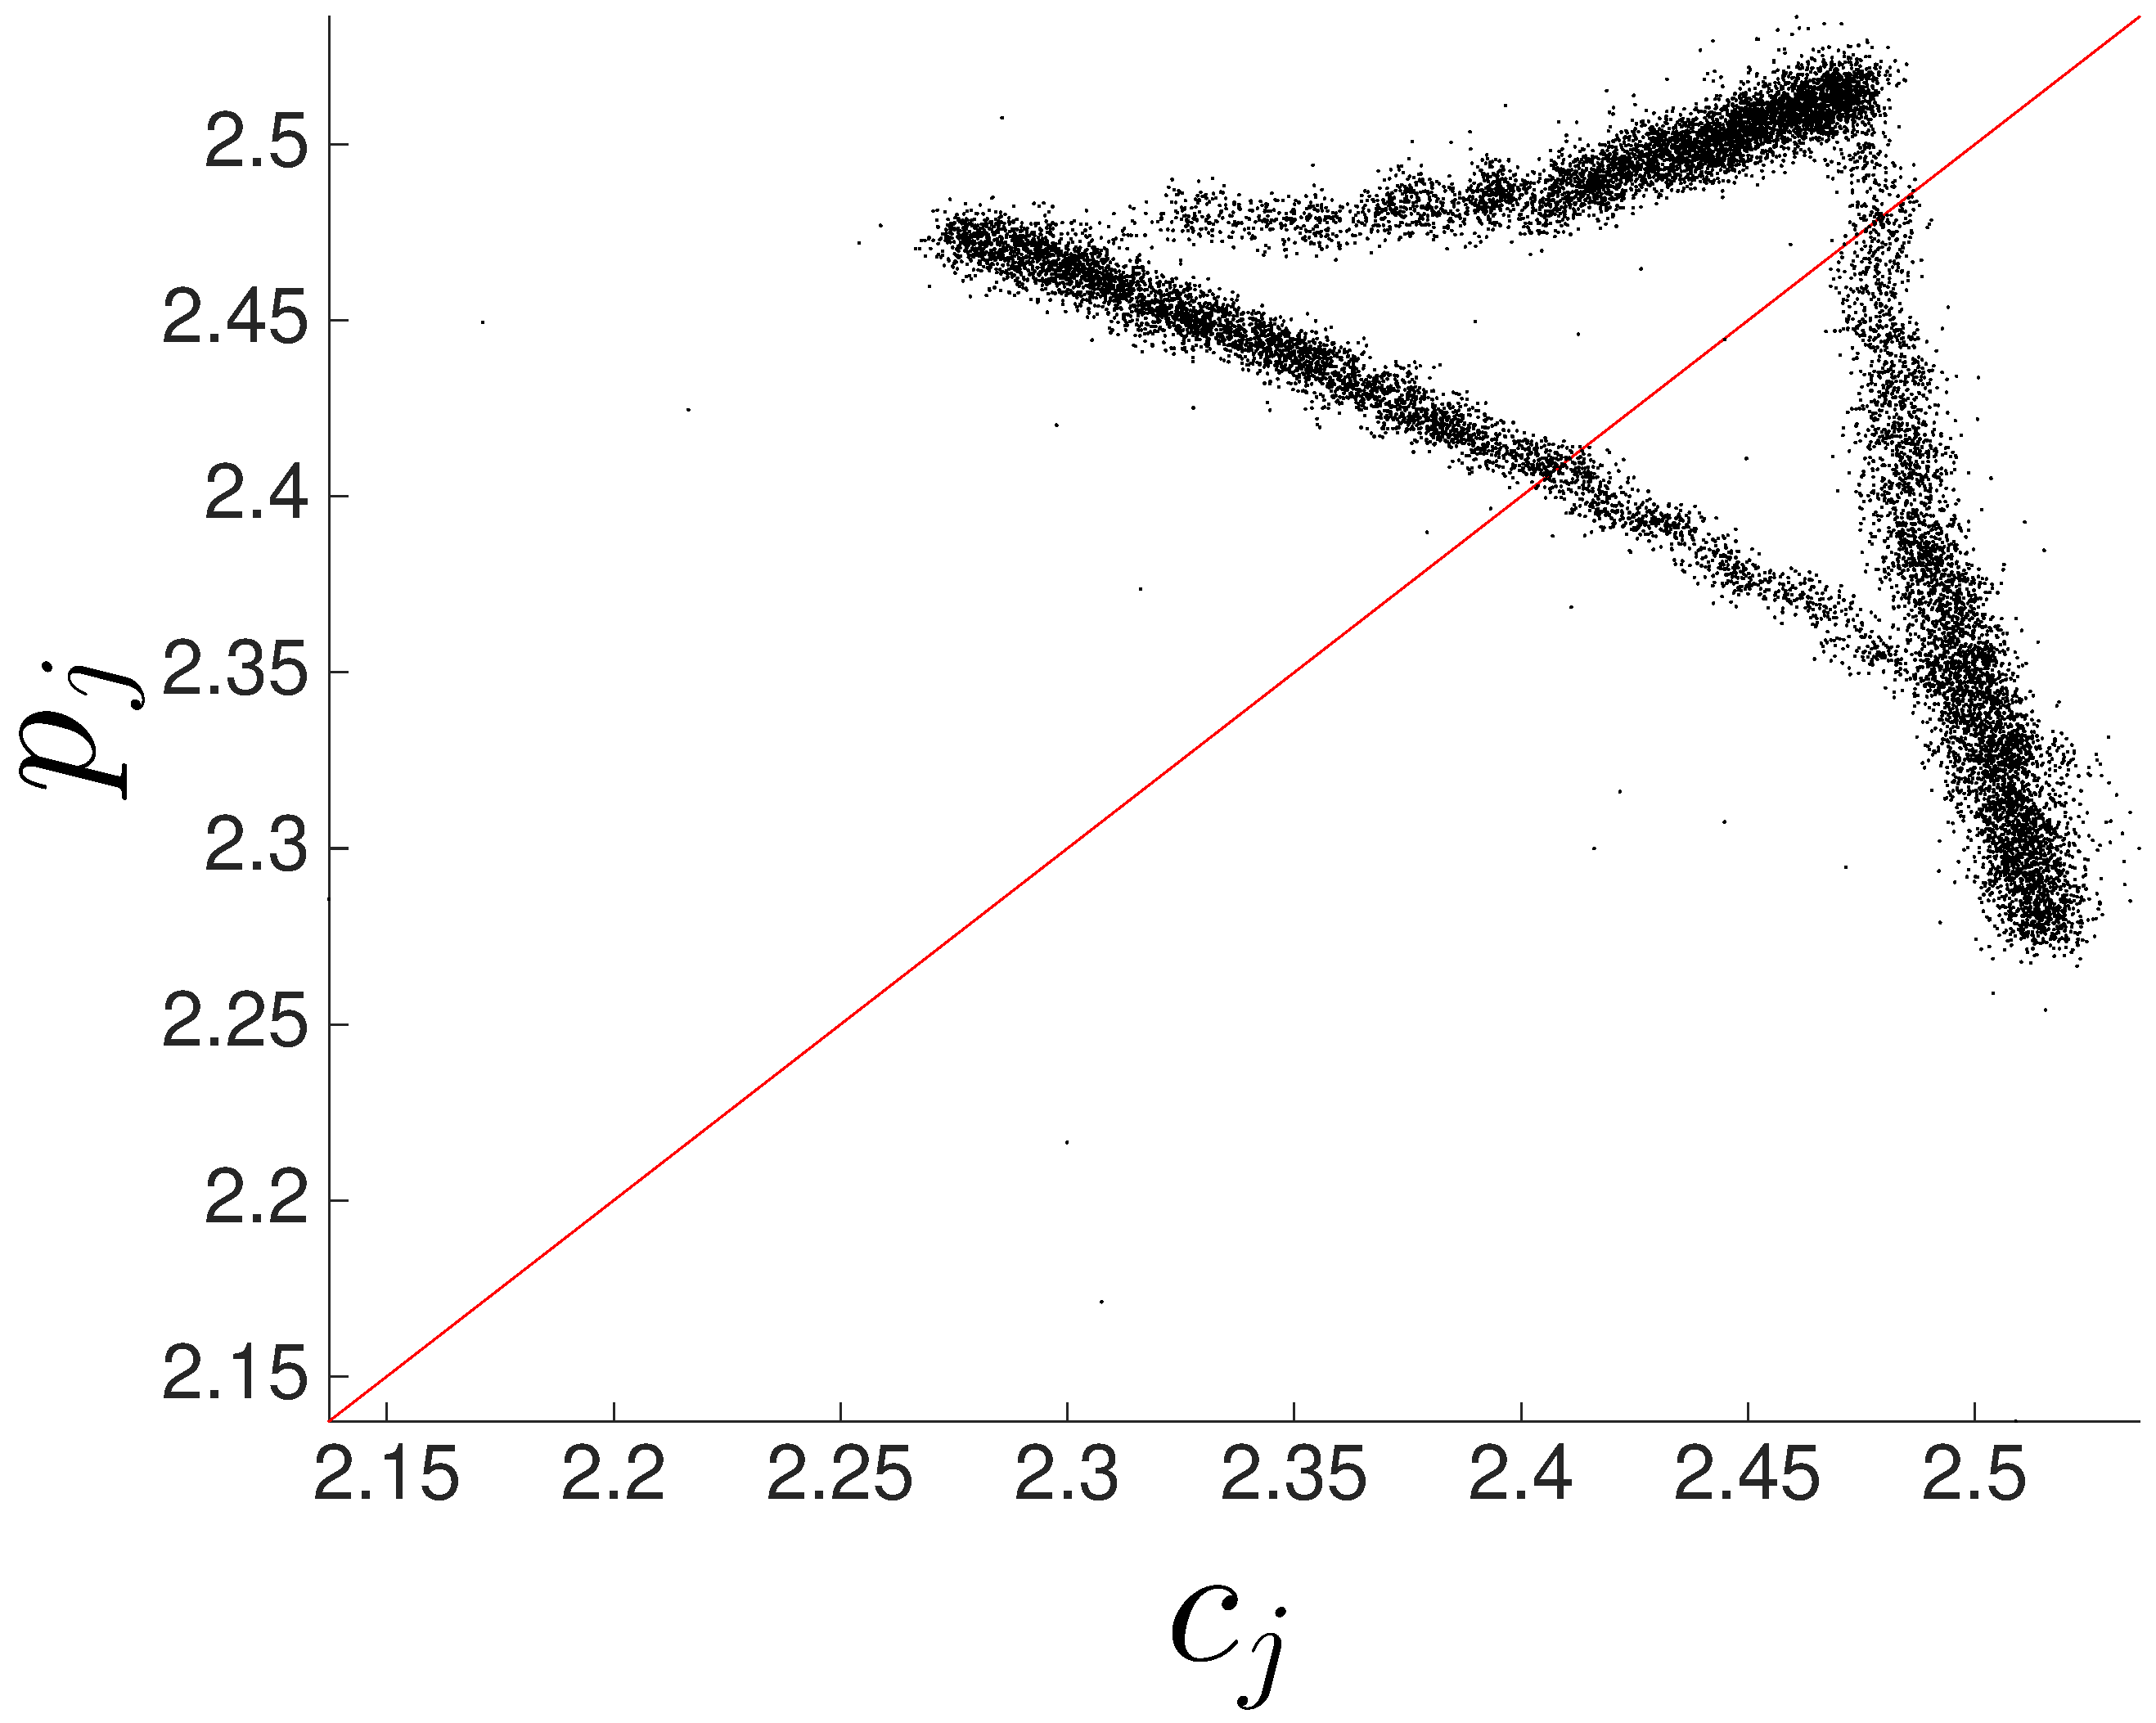
\includegraphics[width=0.6\columnwidth]{figs/colRWForecast} &
    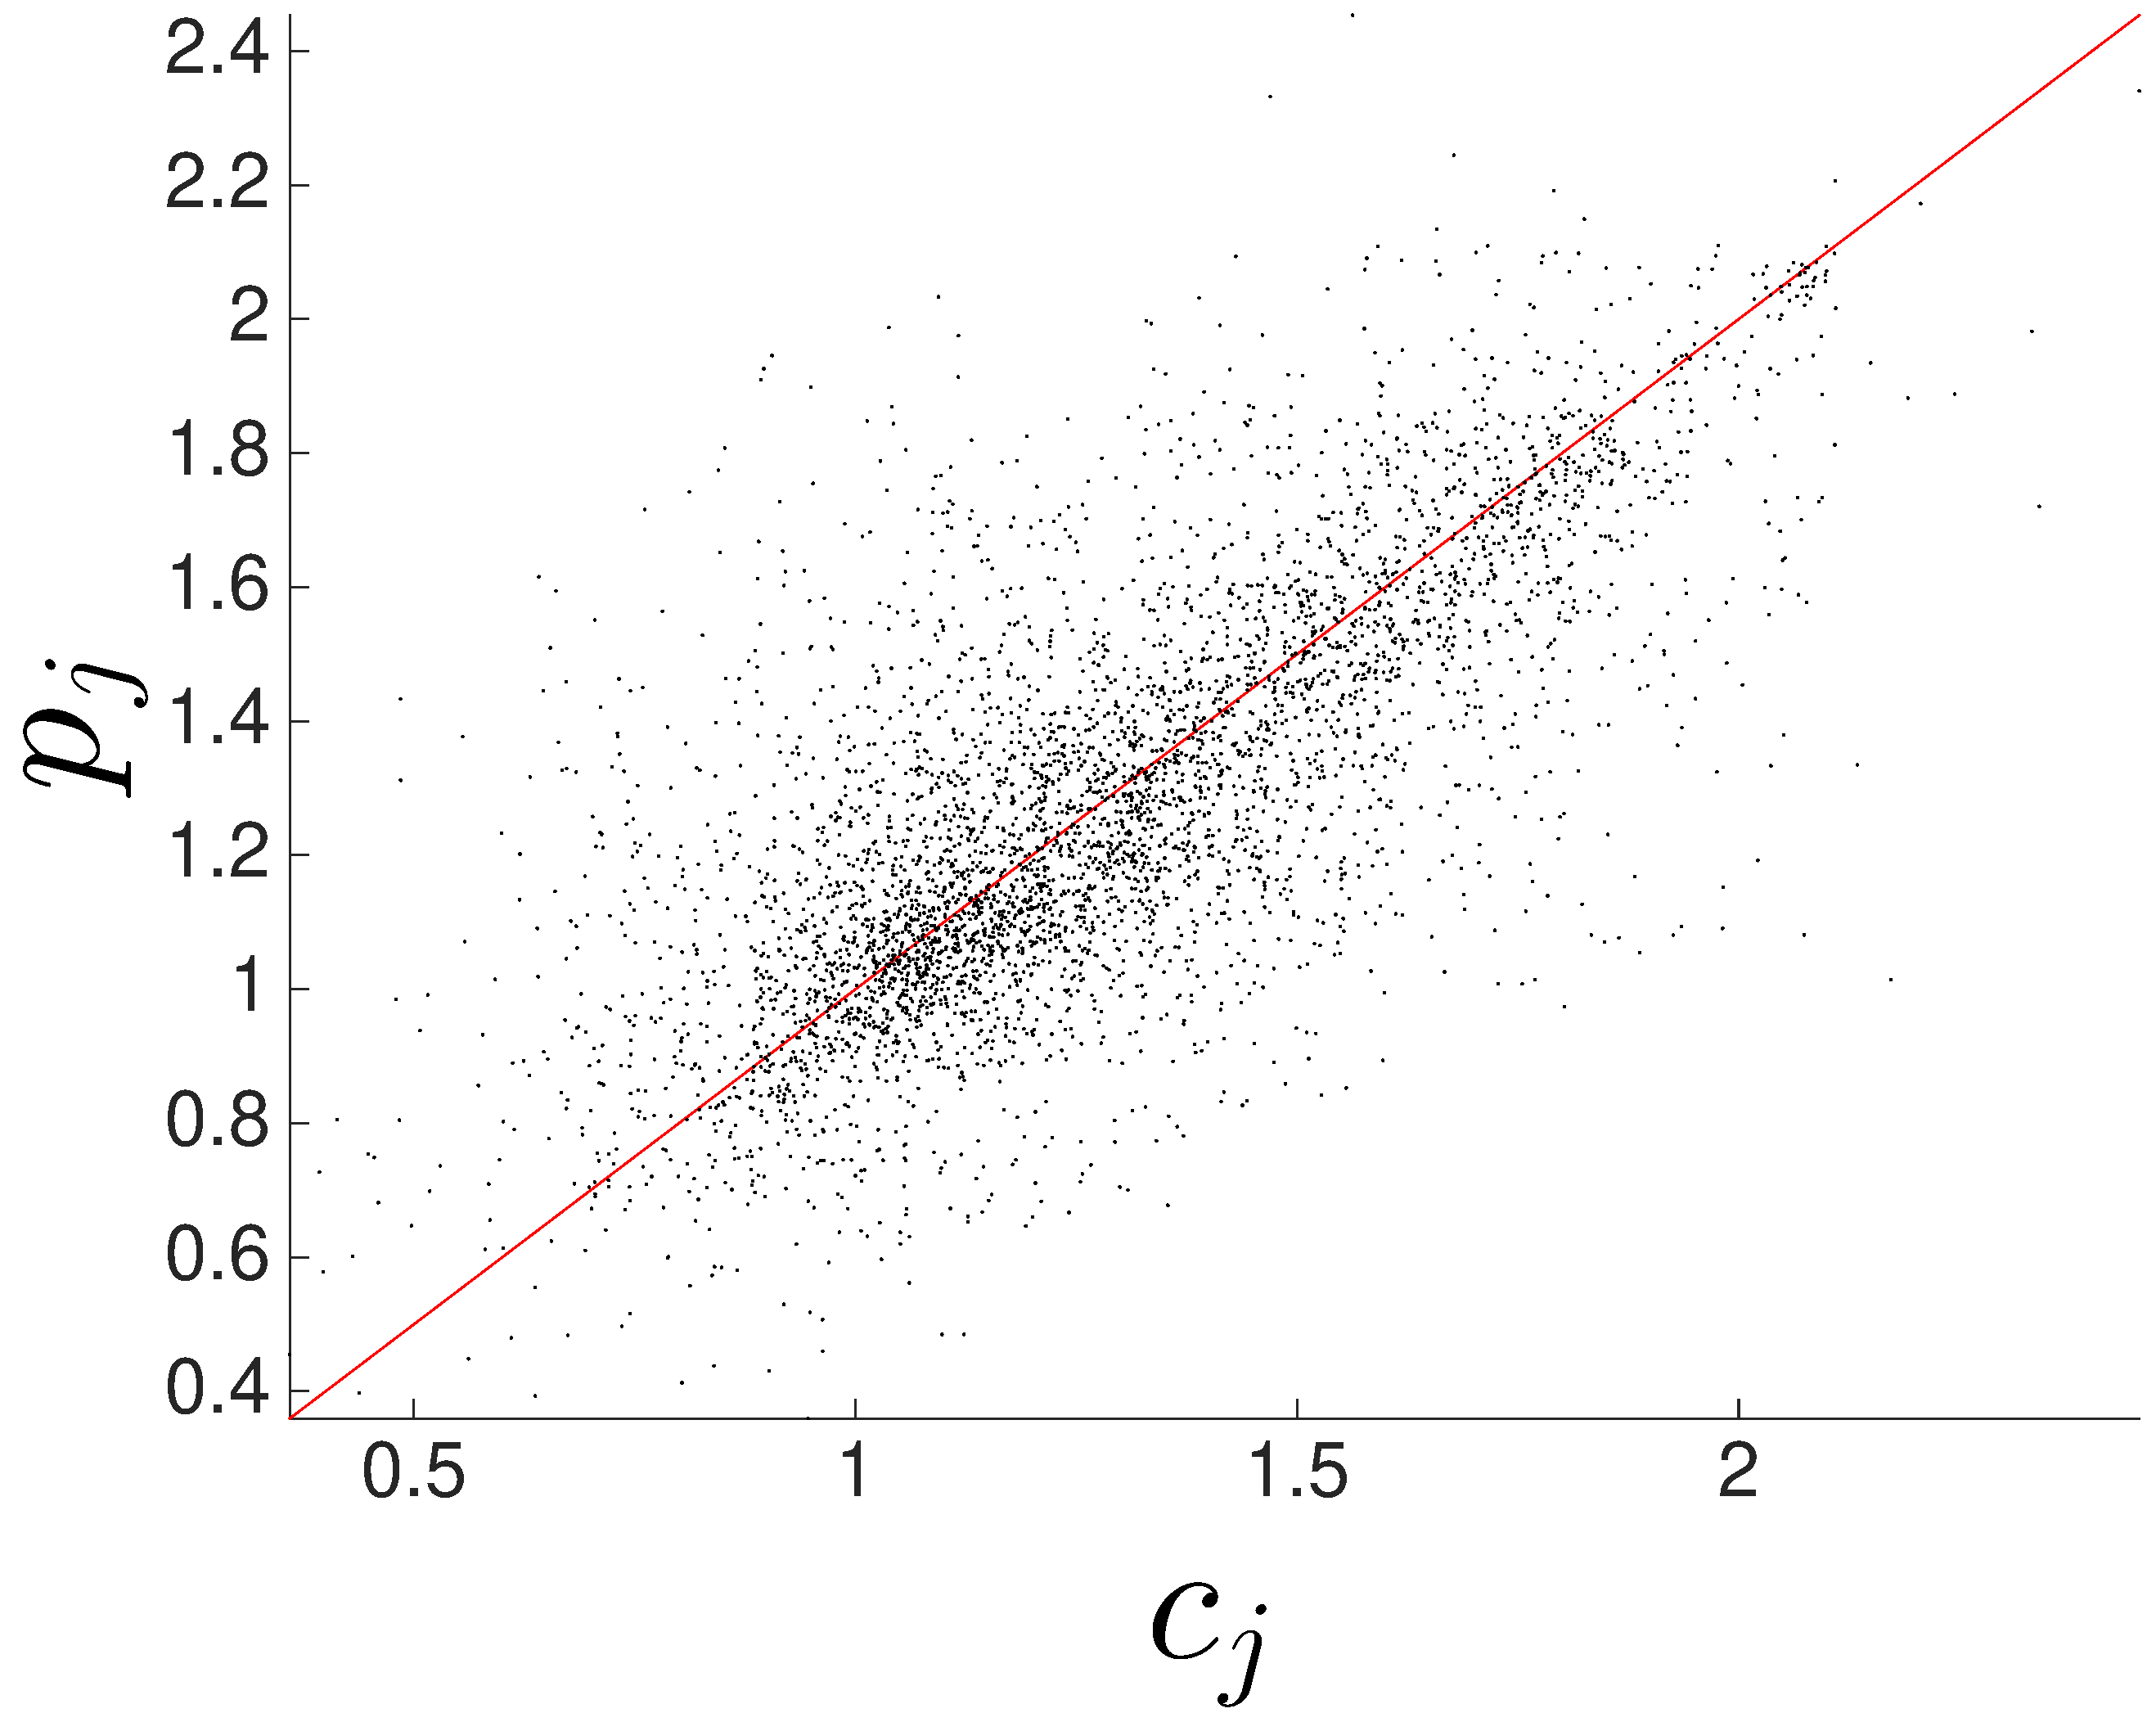
\includegraphics[width=0.6\columnwidth]{figs/gccRWForecast} &
    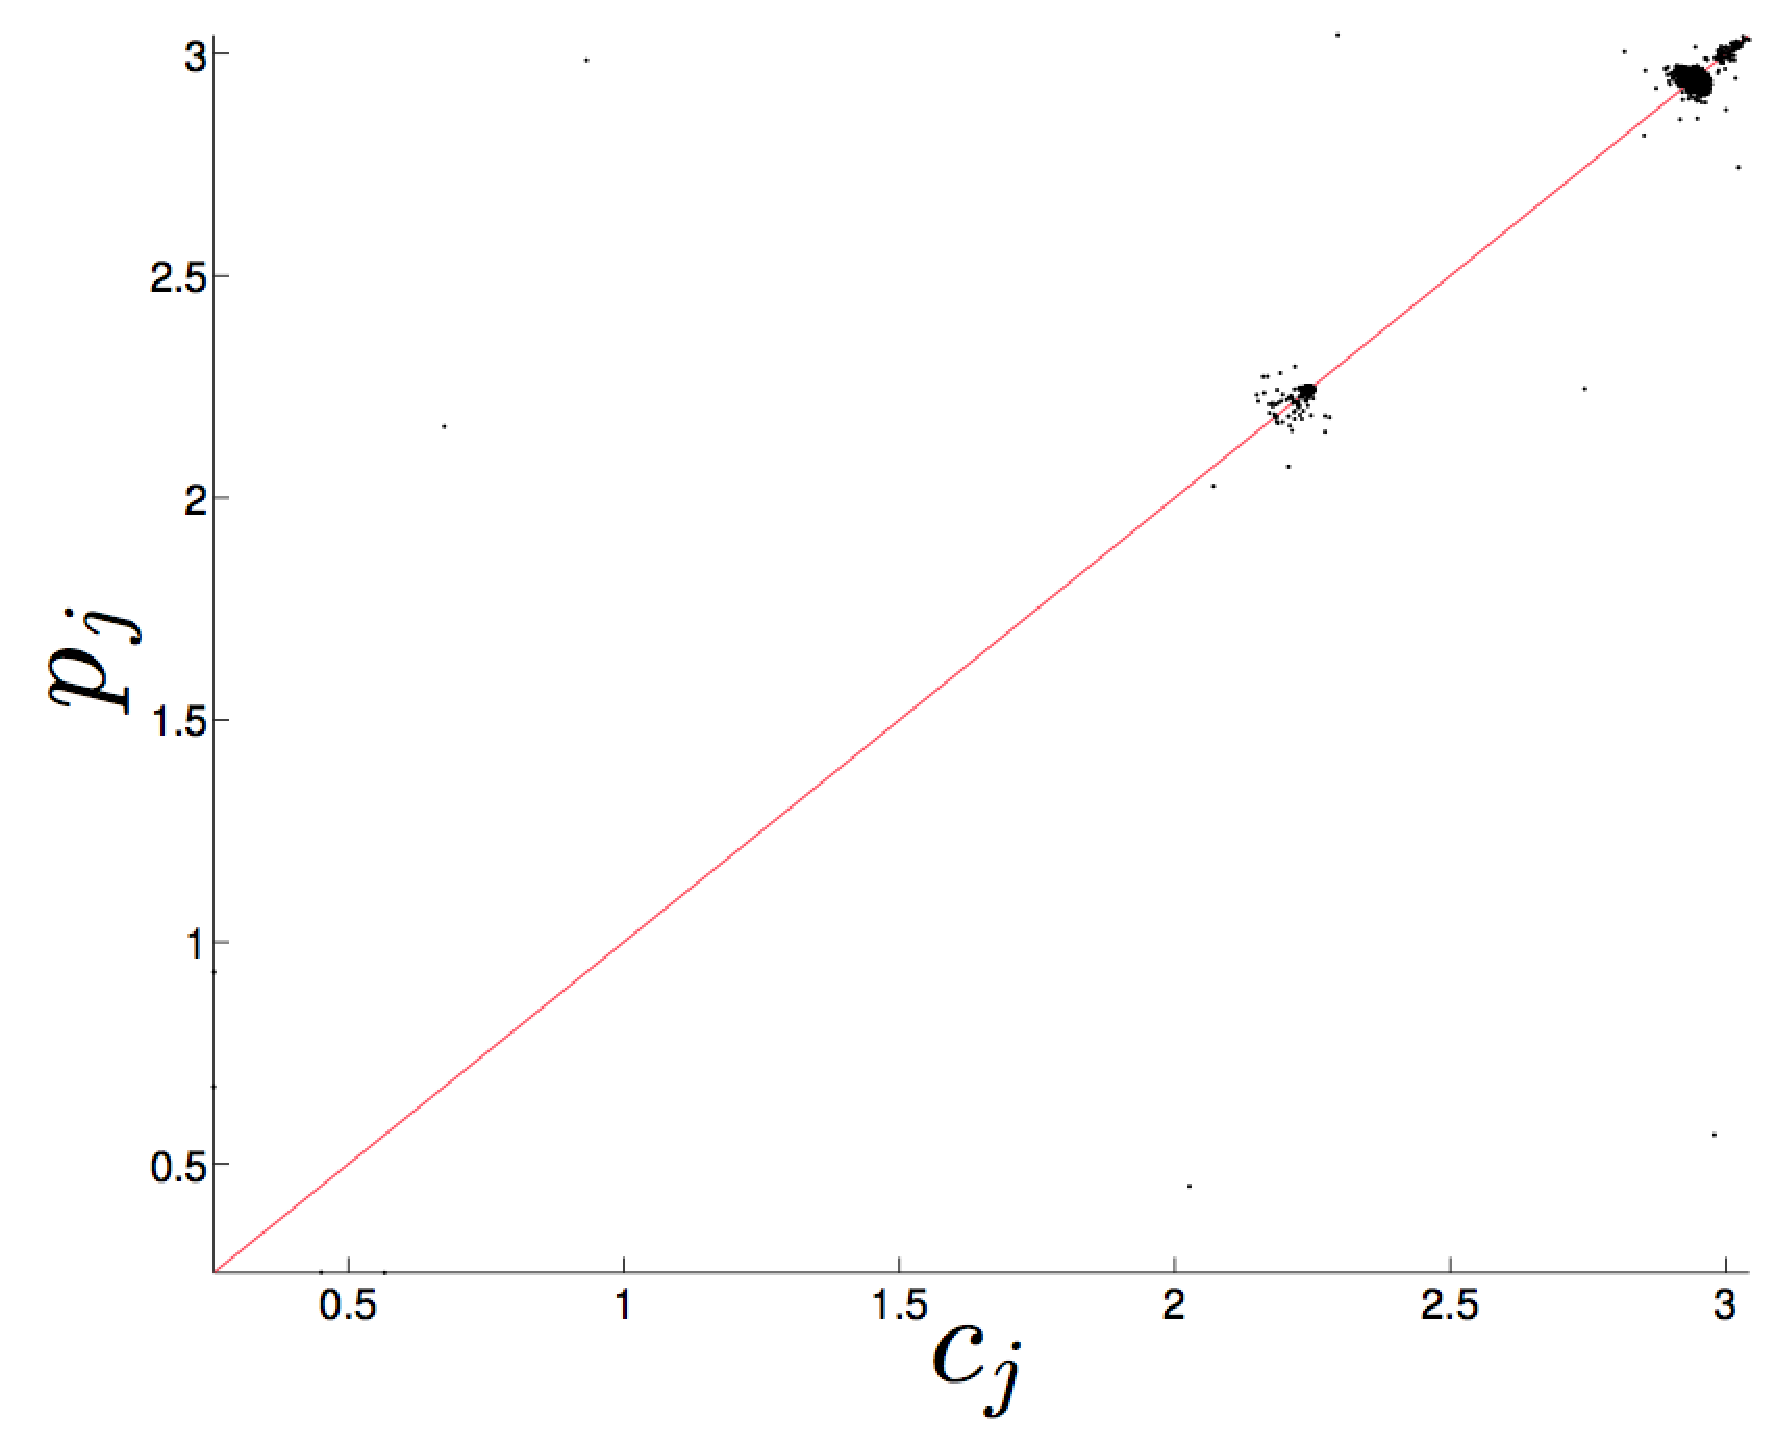
\includegraphics[width=0.6\columnwidth]{figs/svdfiveRWForecast} \\
    \rotatebox{90}{\large \naive} &
    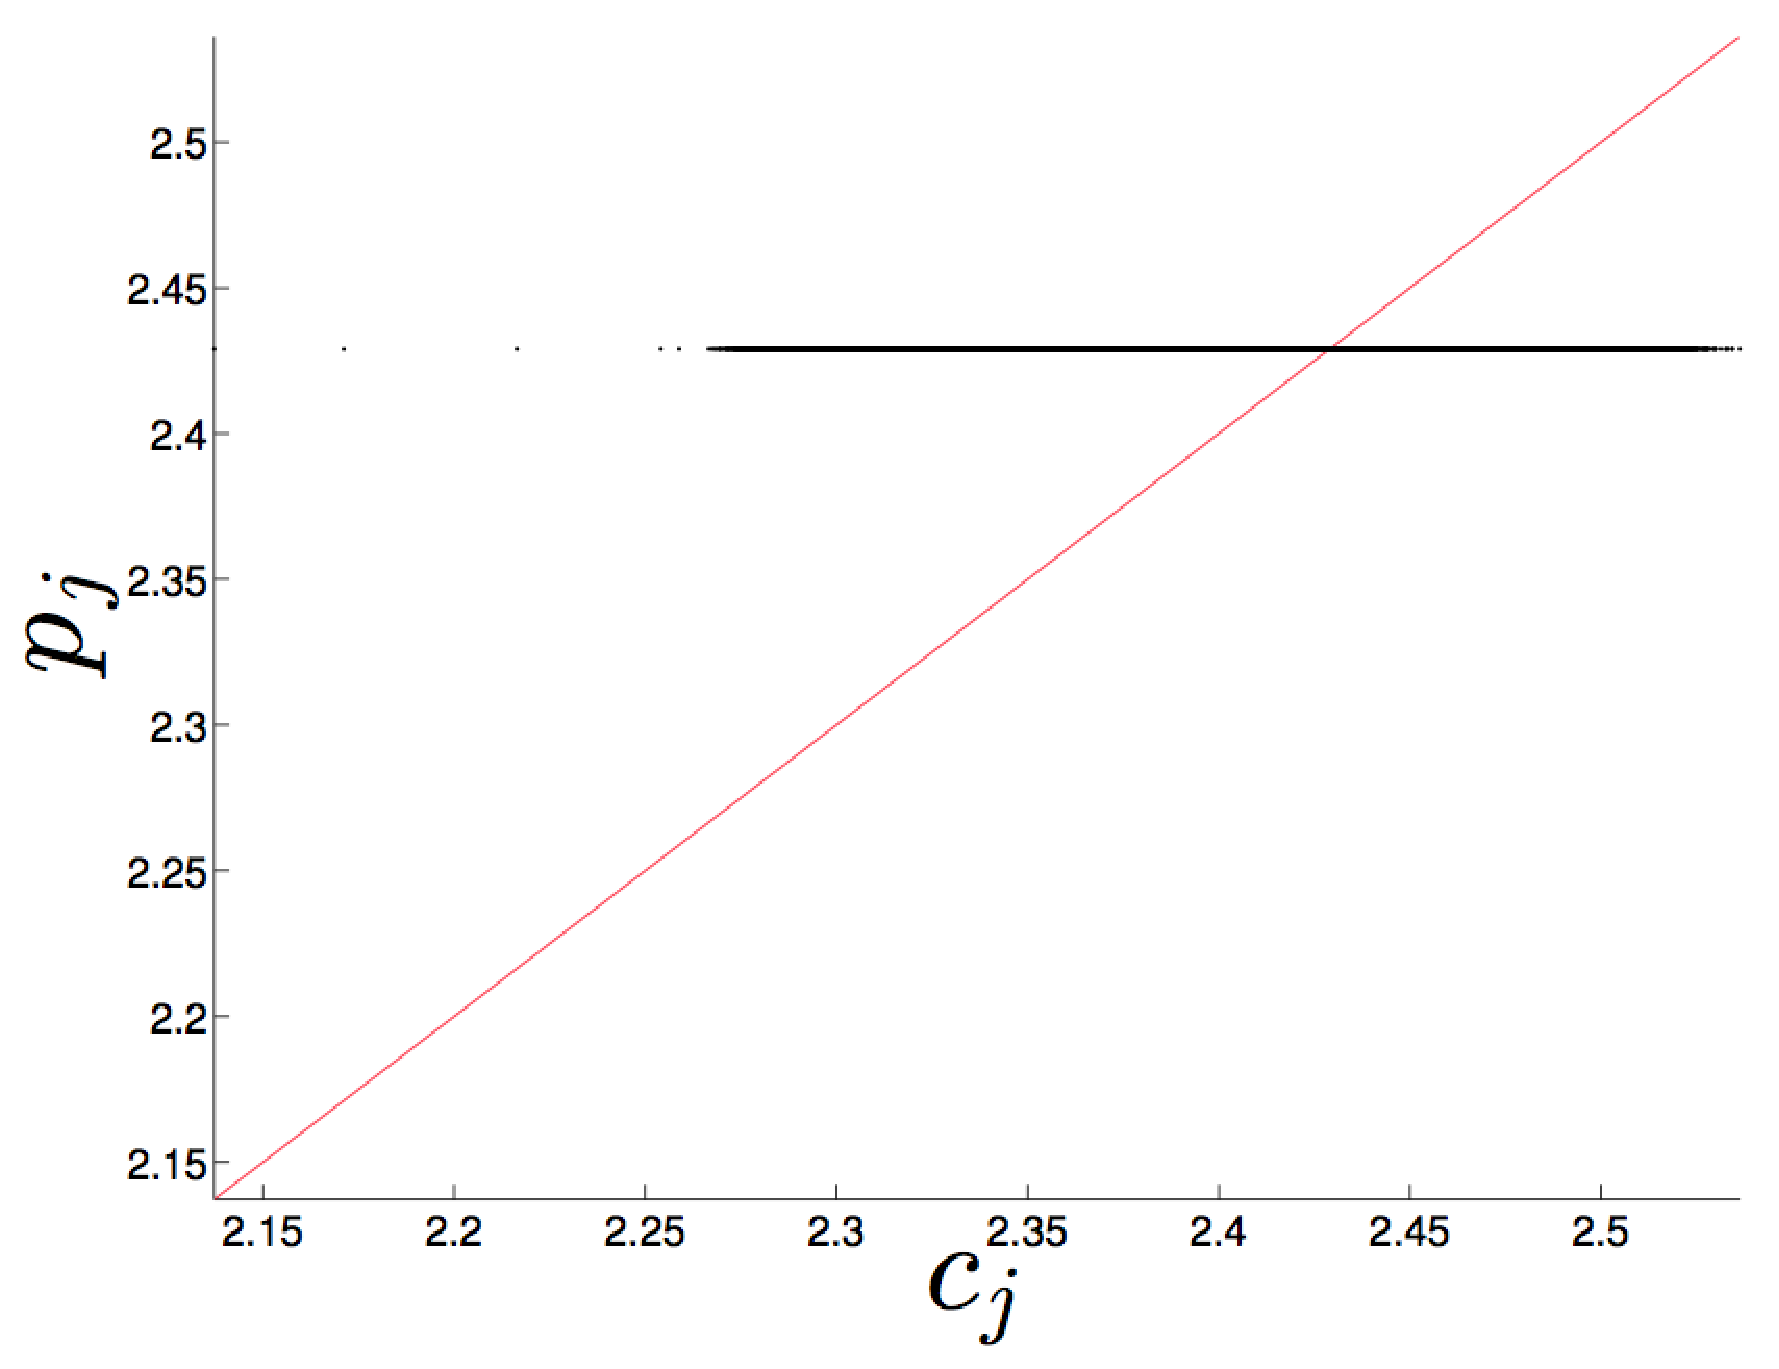
\includegraphics[width=0.6\columnwidth]{figs/colMeanForecast} &
    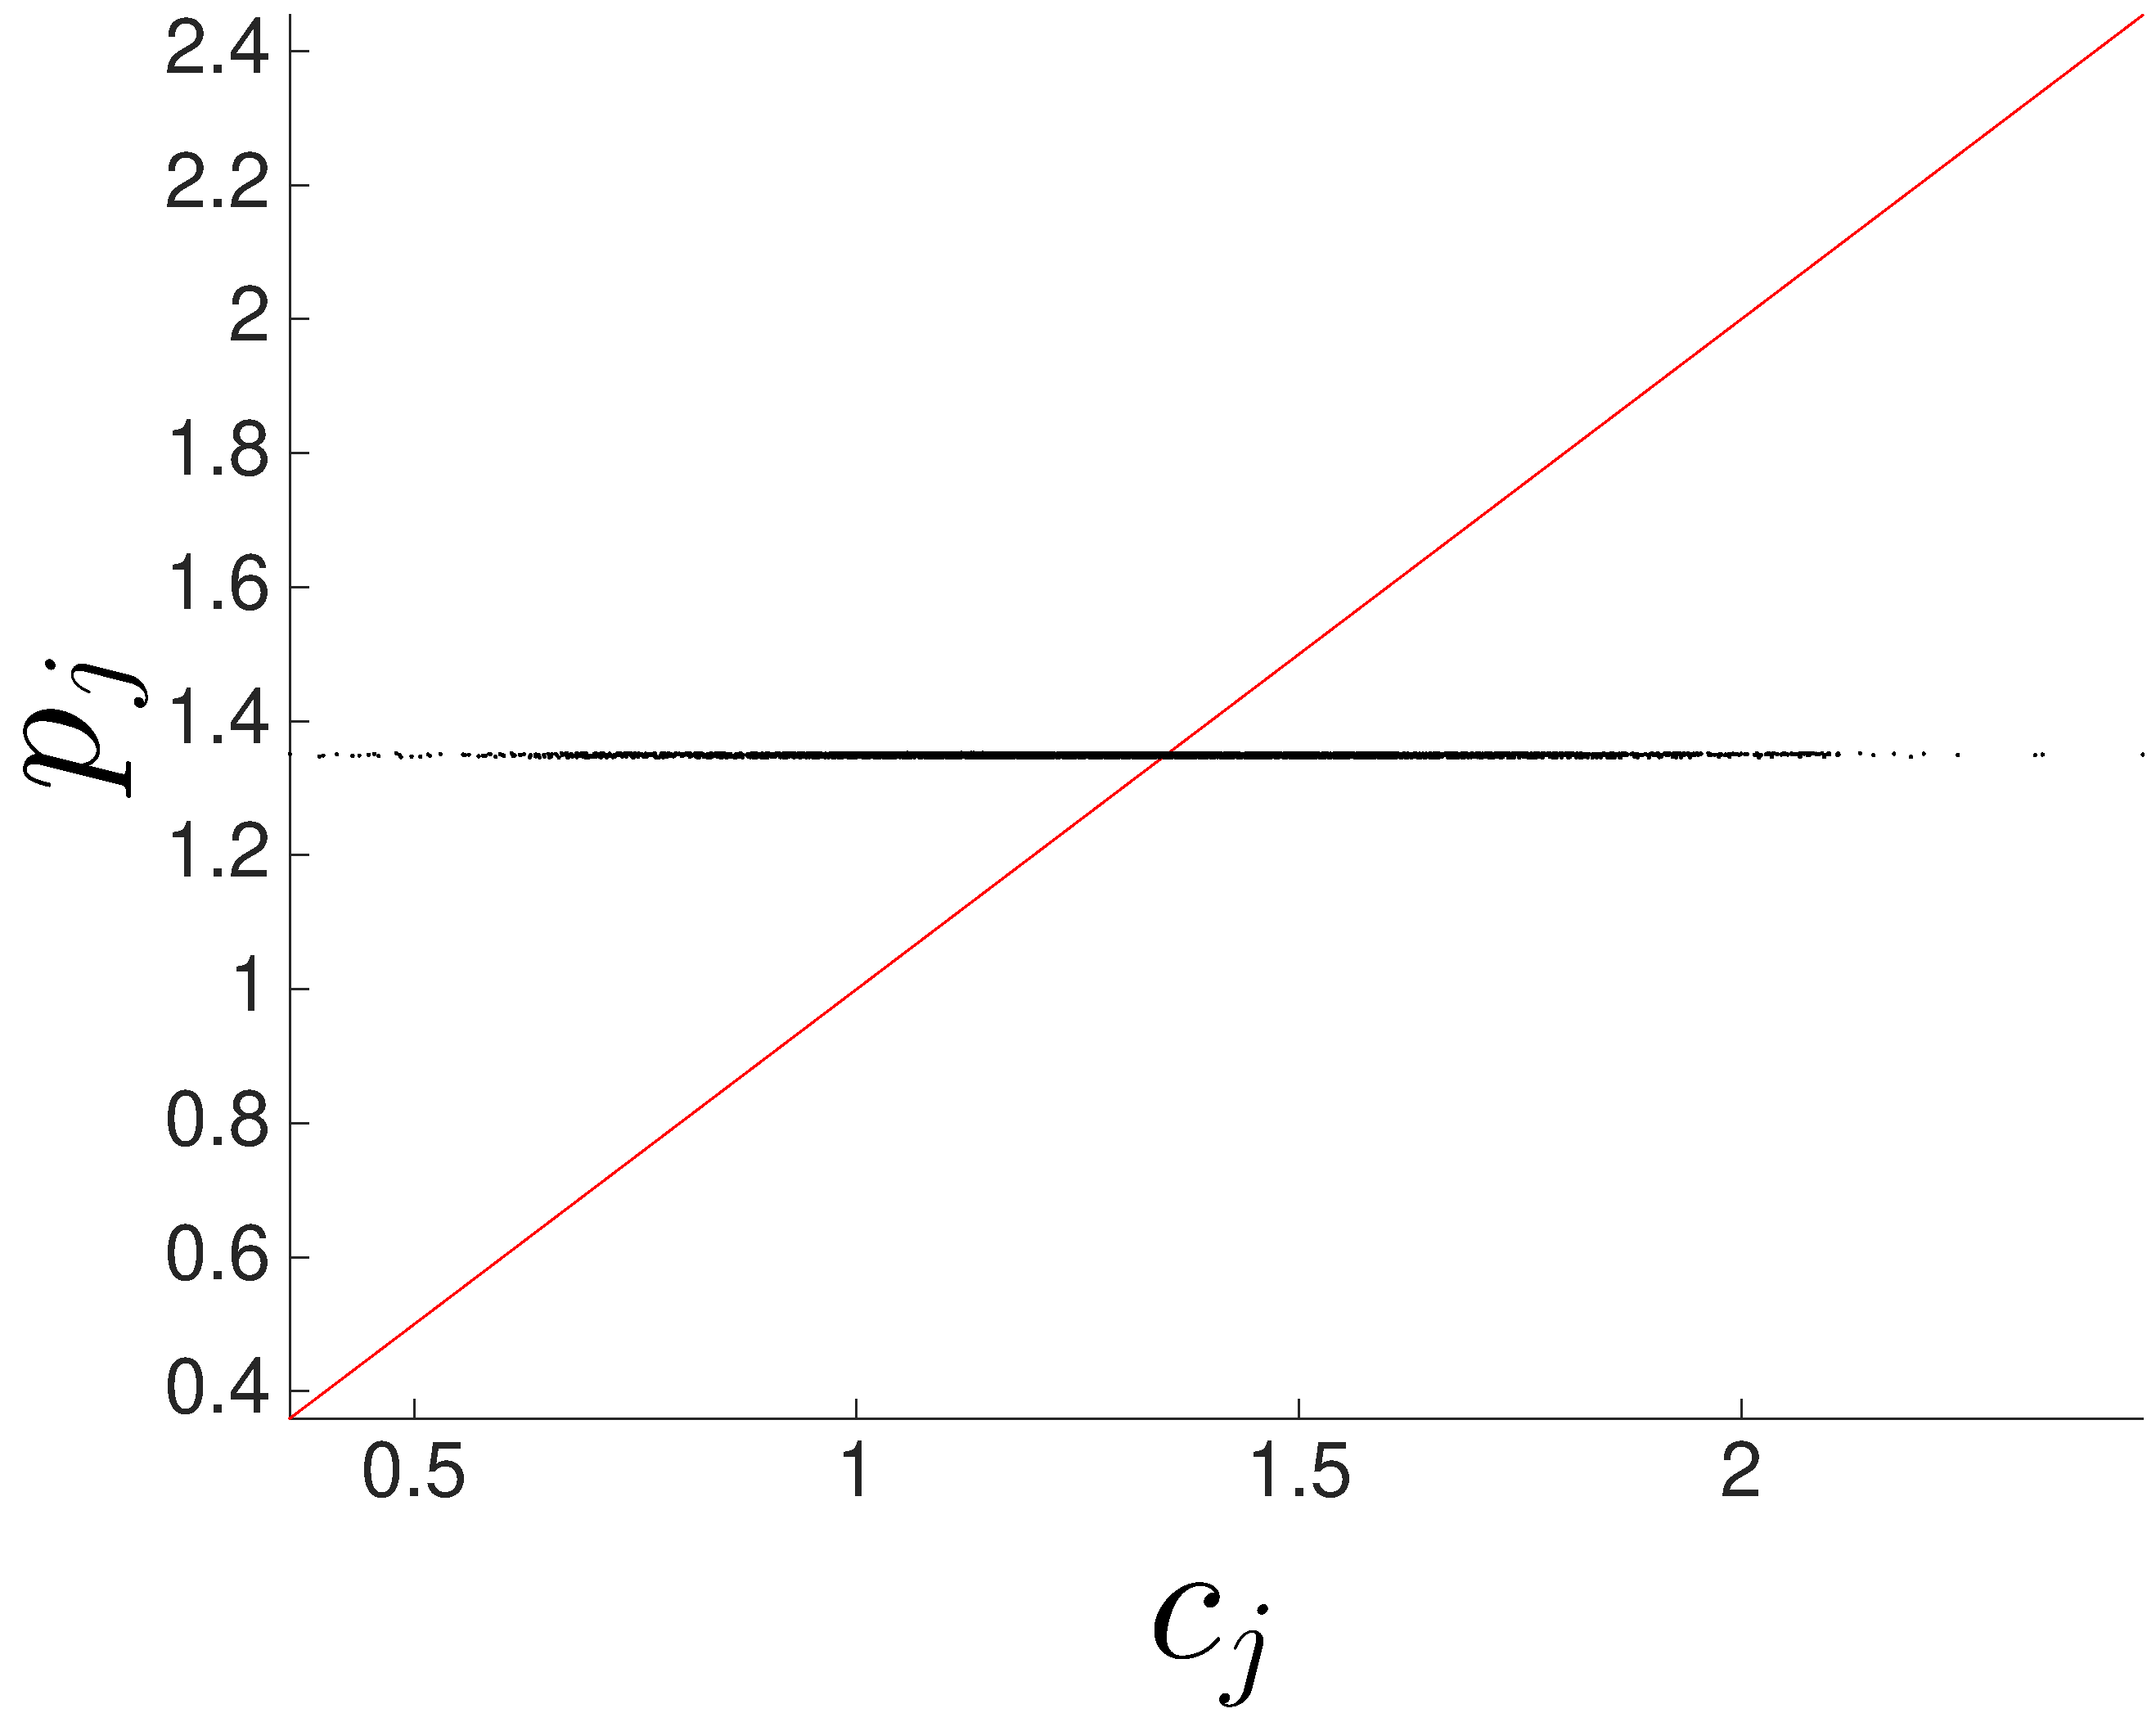
\includegraphics[width=0.6\columnwidth]{figs/gccMeanForecast} &
    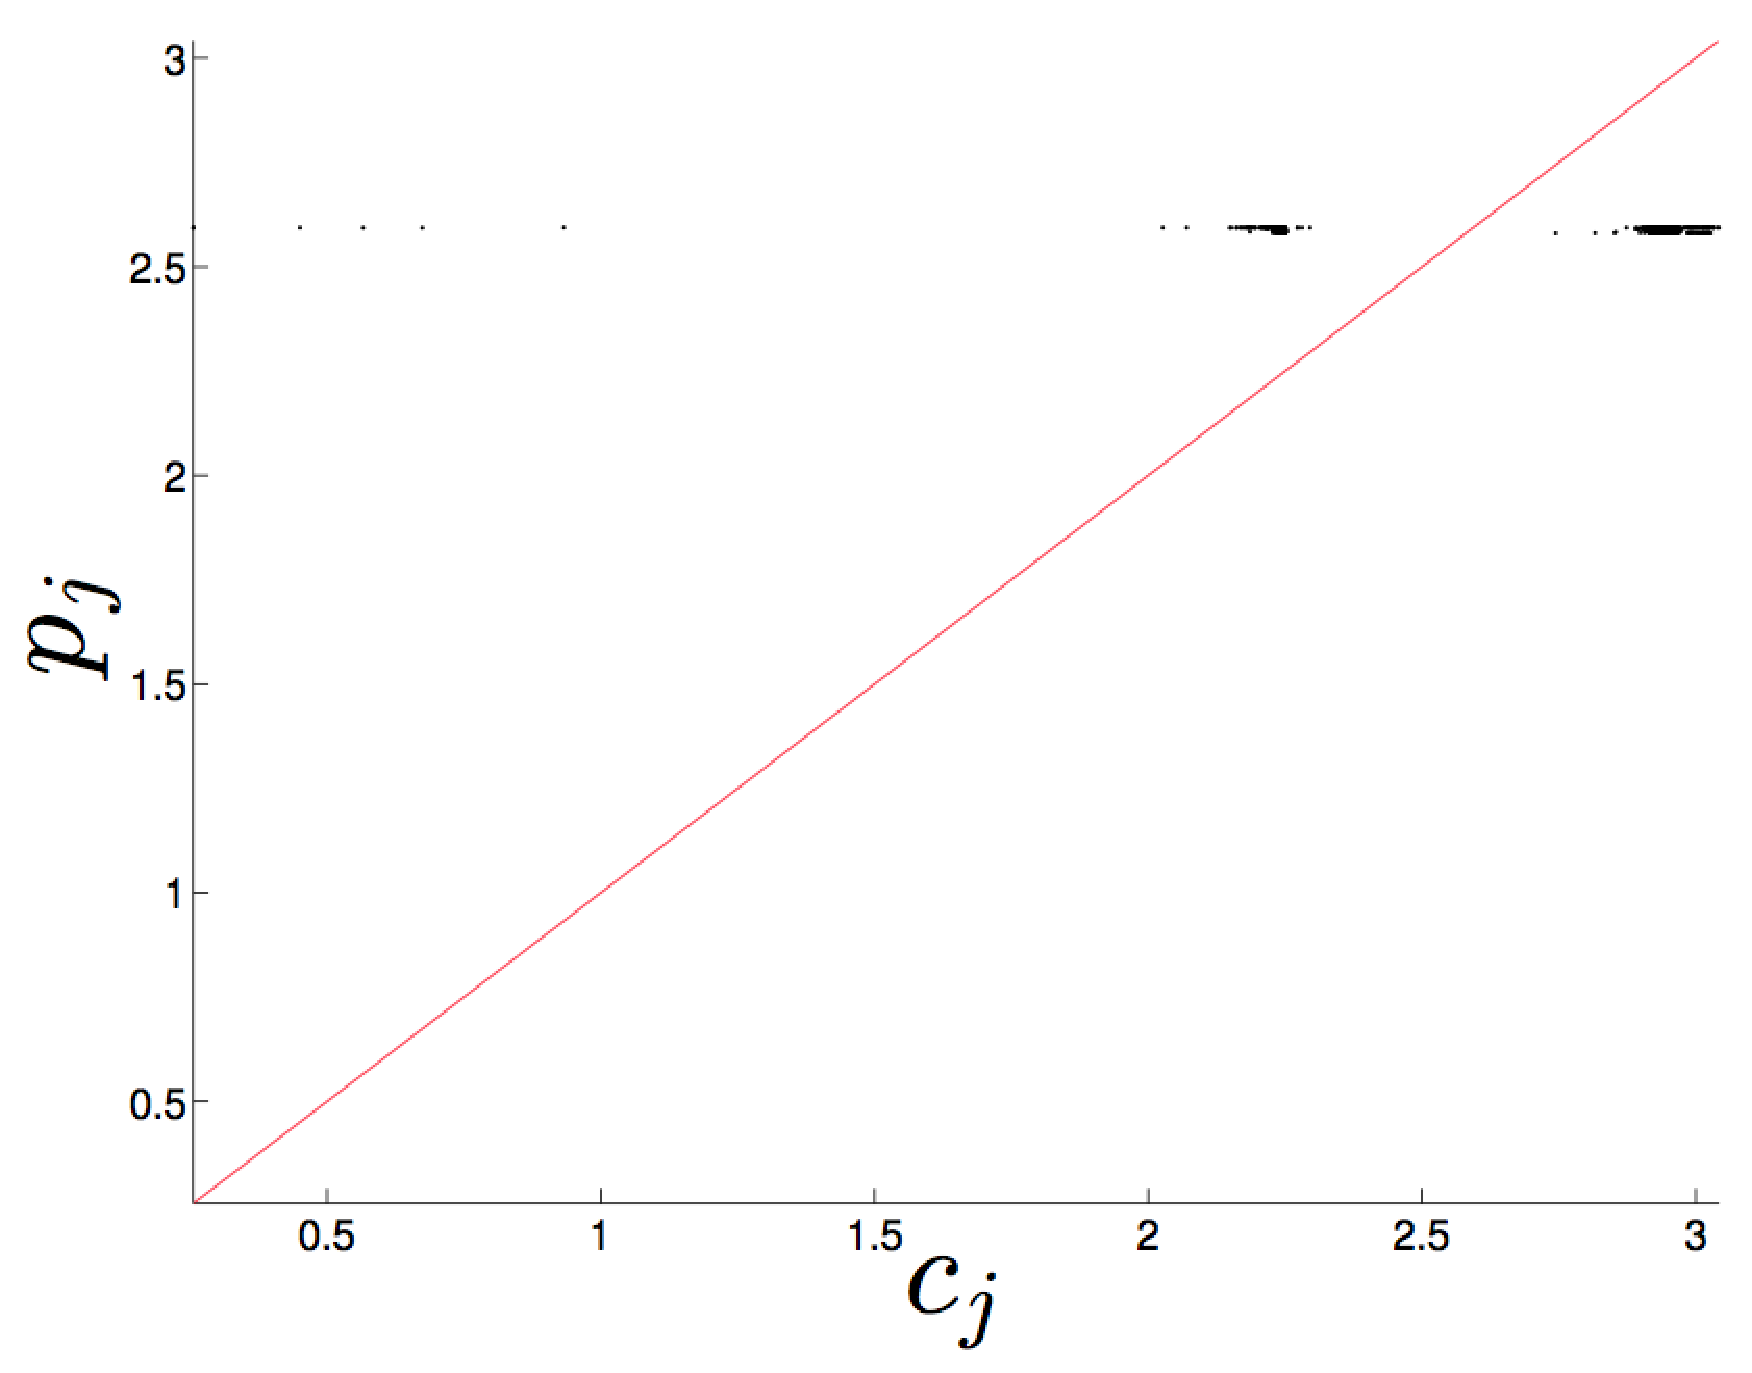
\includegraphics[width=0.6\columnwidth]{figs/svdfiveMeanForecast} \\
    \rotatebox{90}{\large \arima} &
    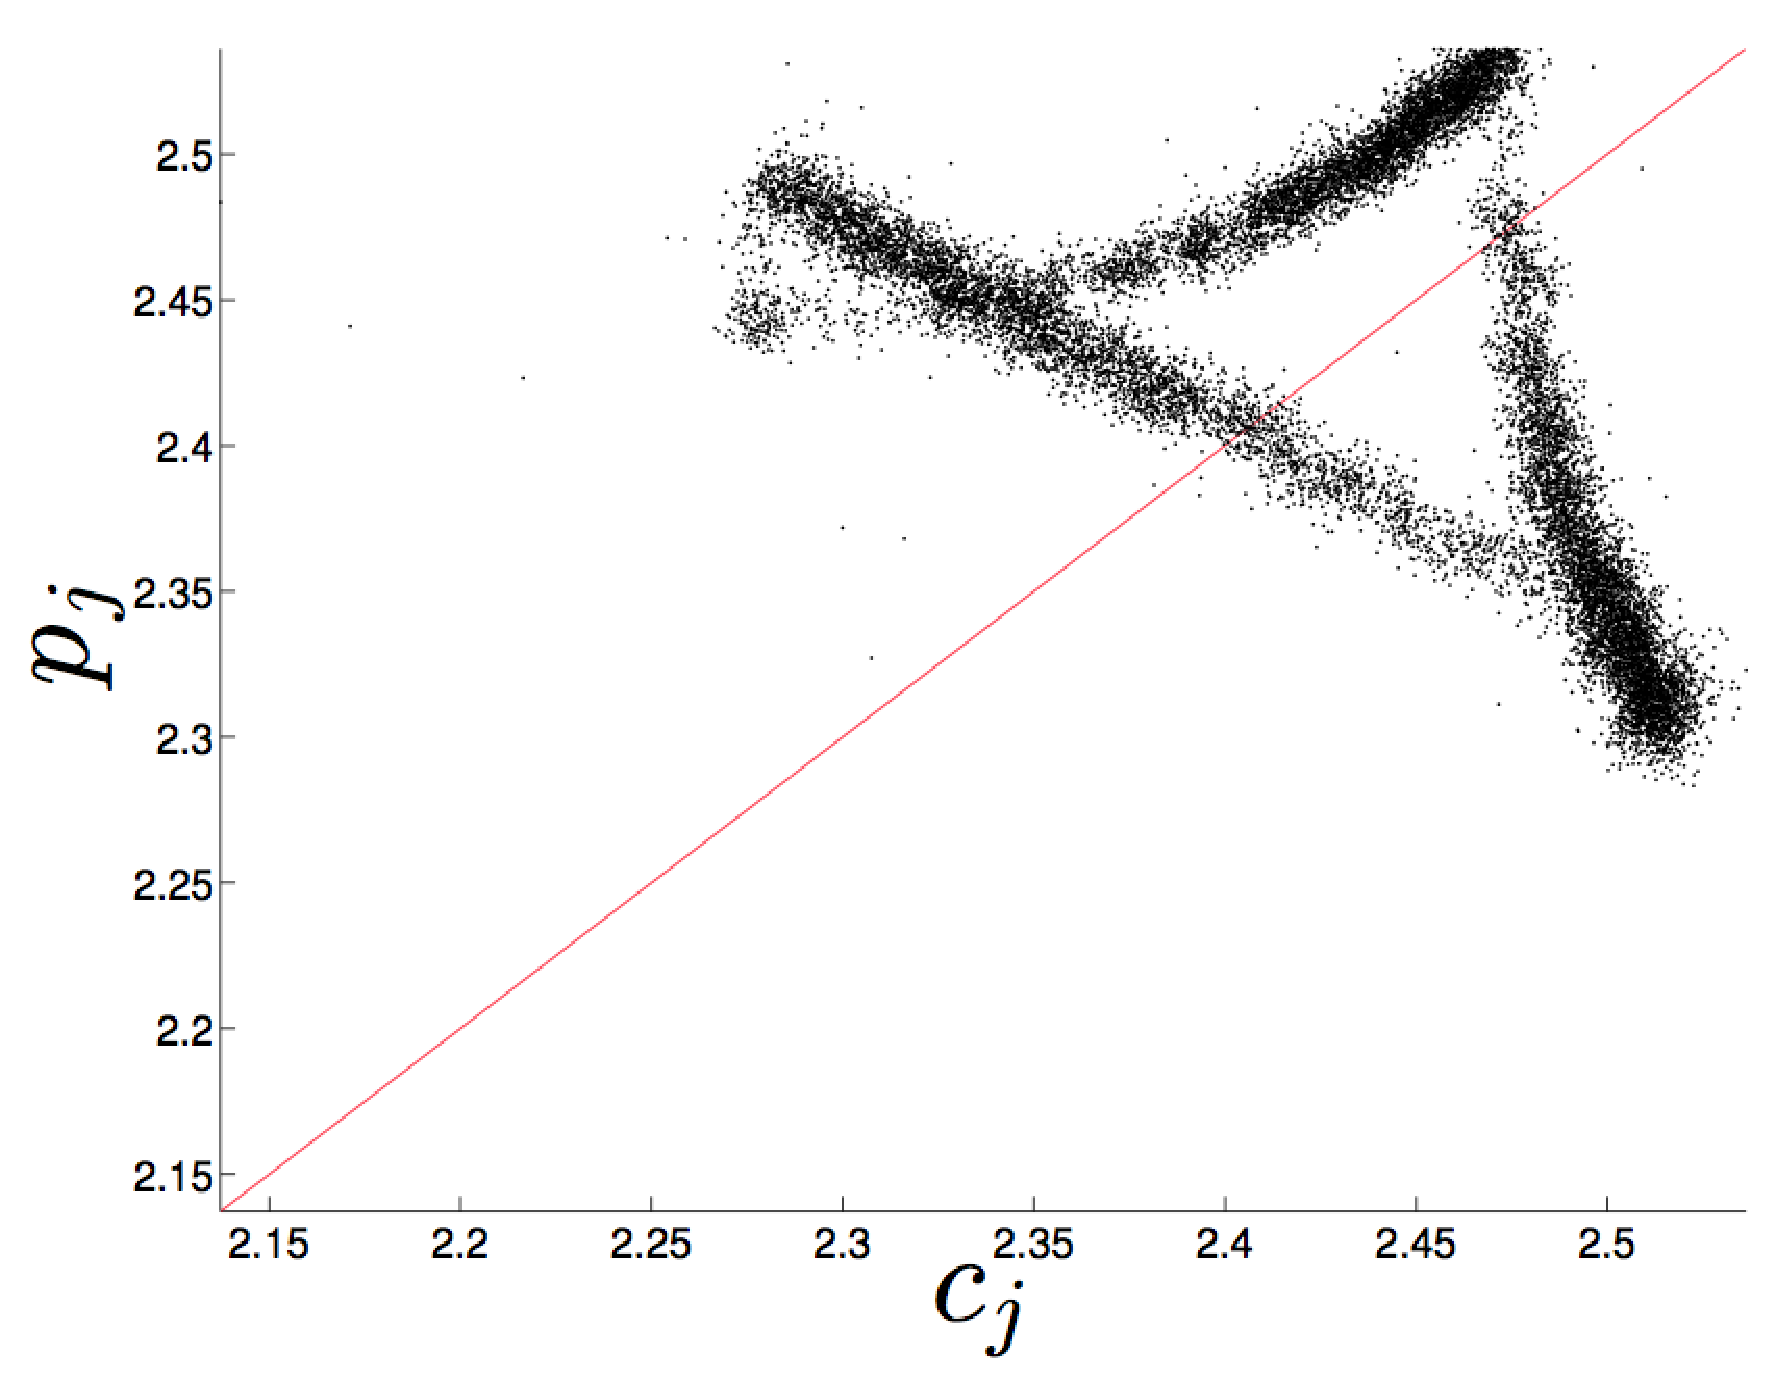
\includegraphics[width=0.6\columnwidth]{figs/colARIMAForecast} &
    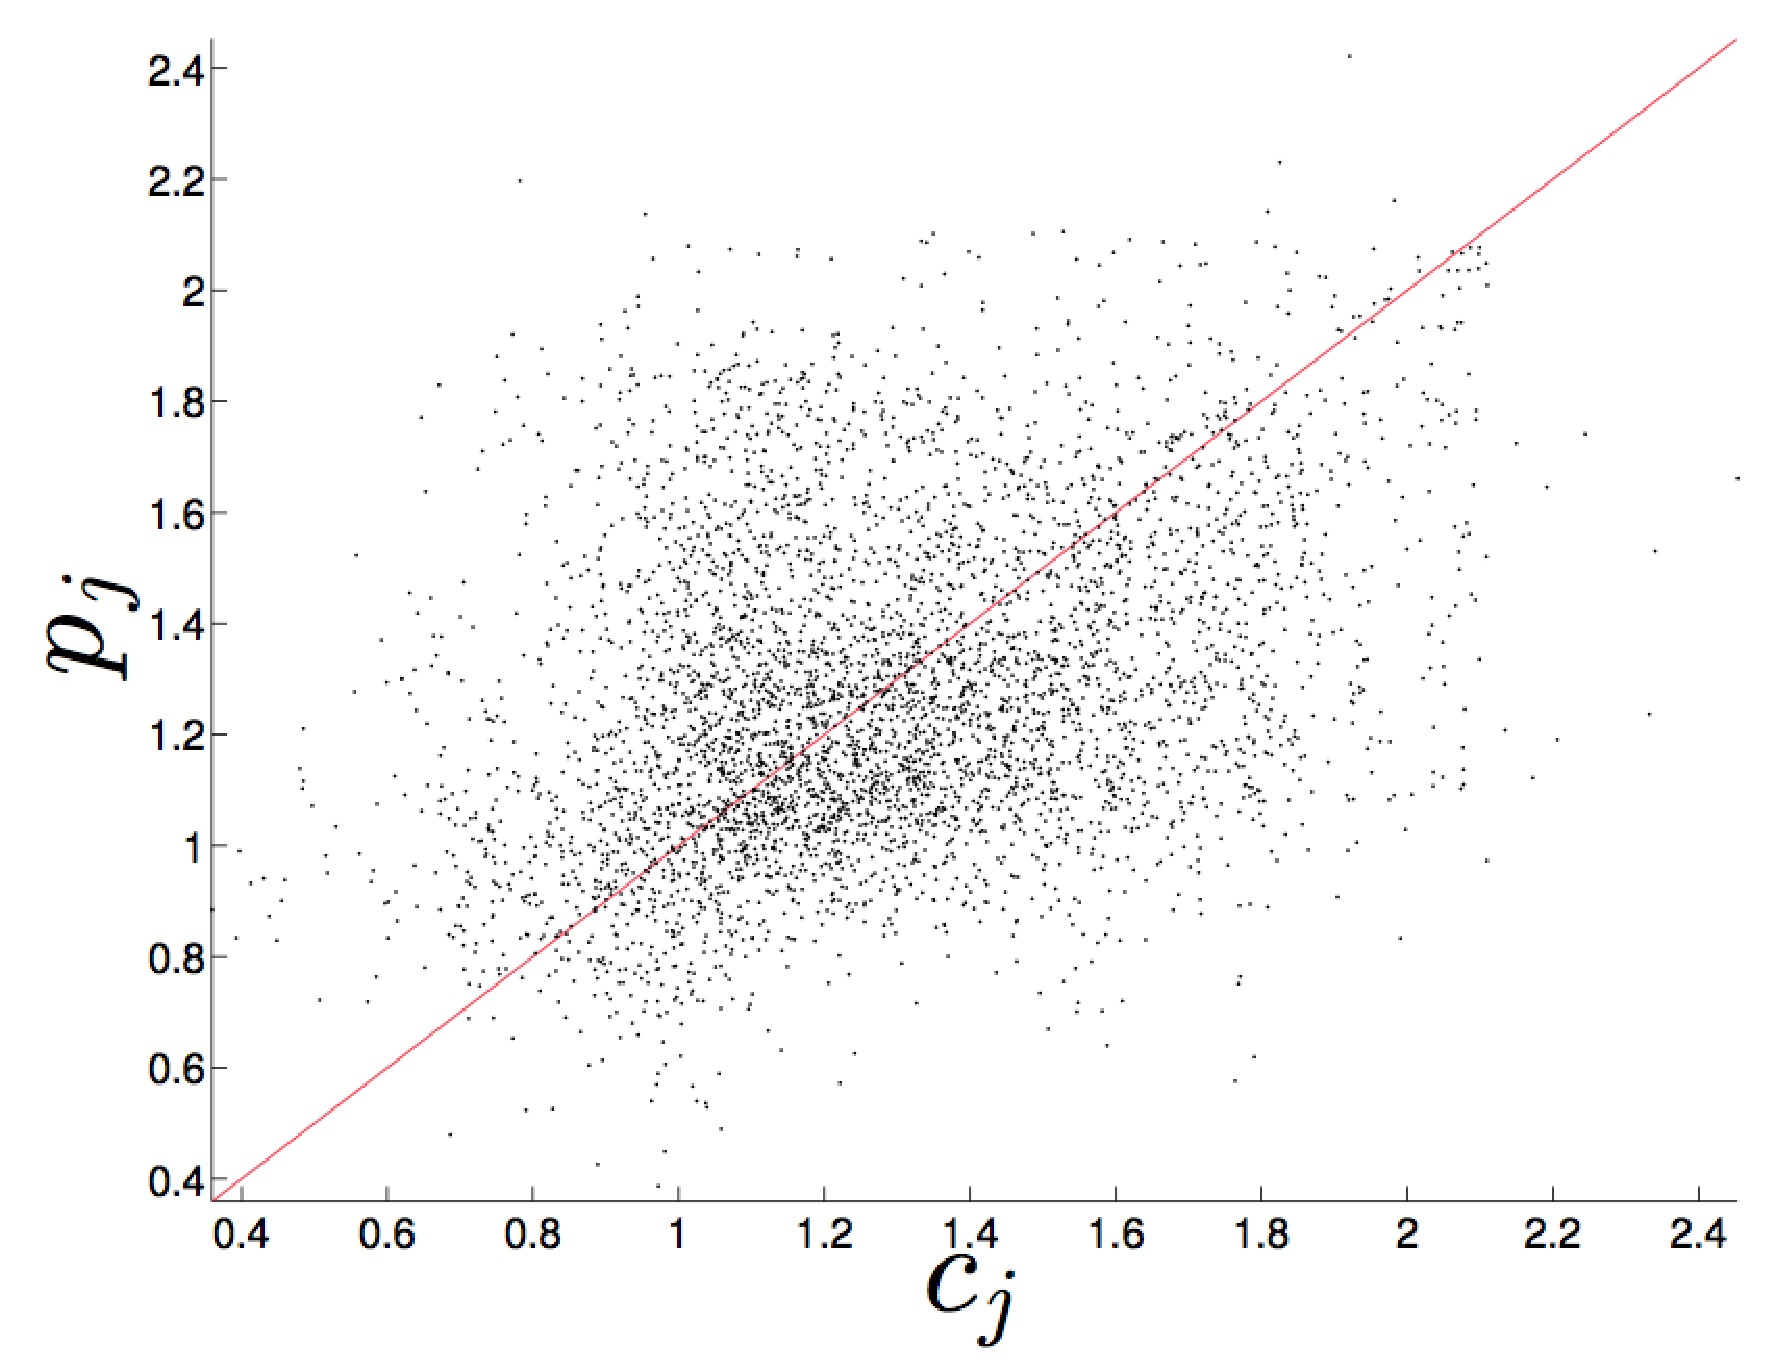
\includegraphics[width=0.6\columnwidth]{figs/gccARIMAForecast} &
    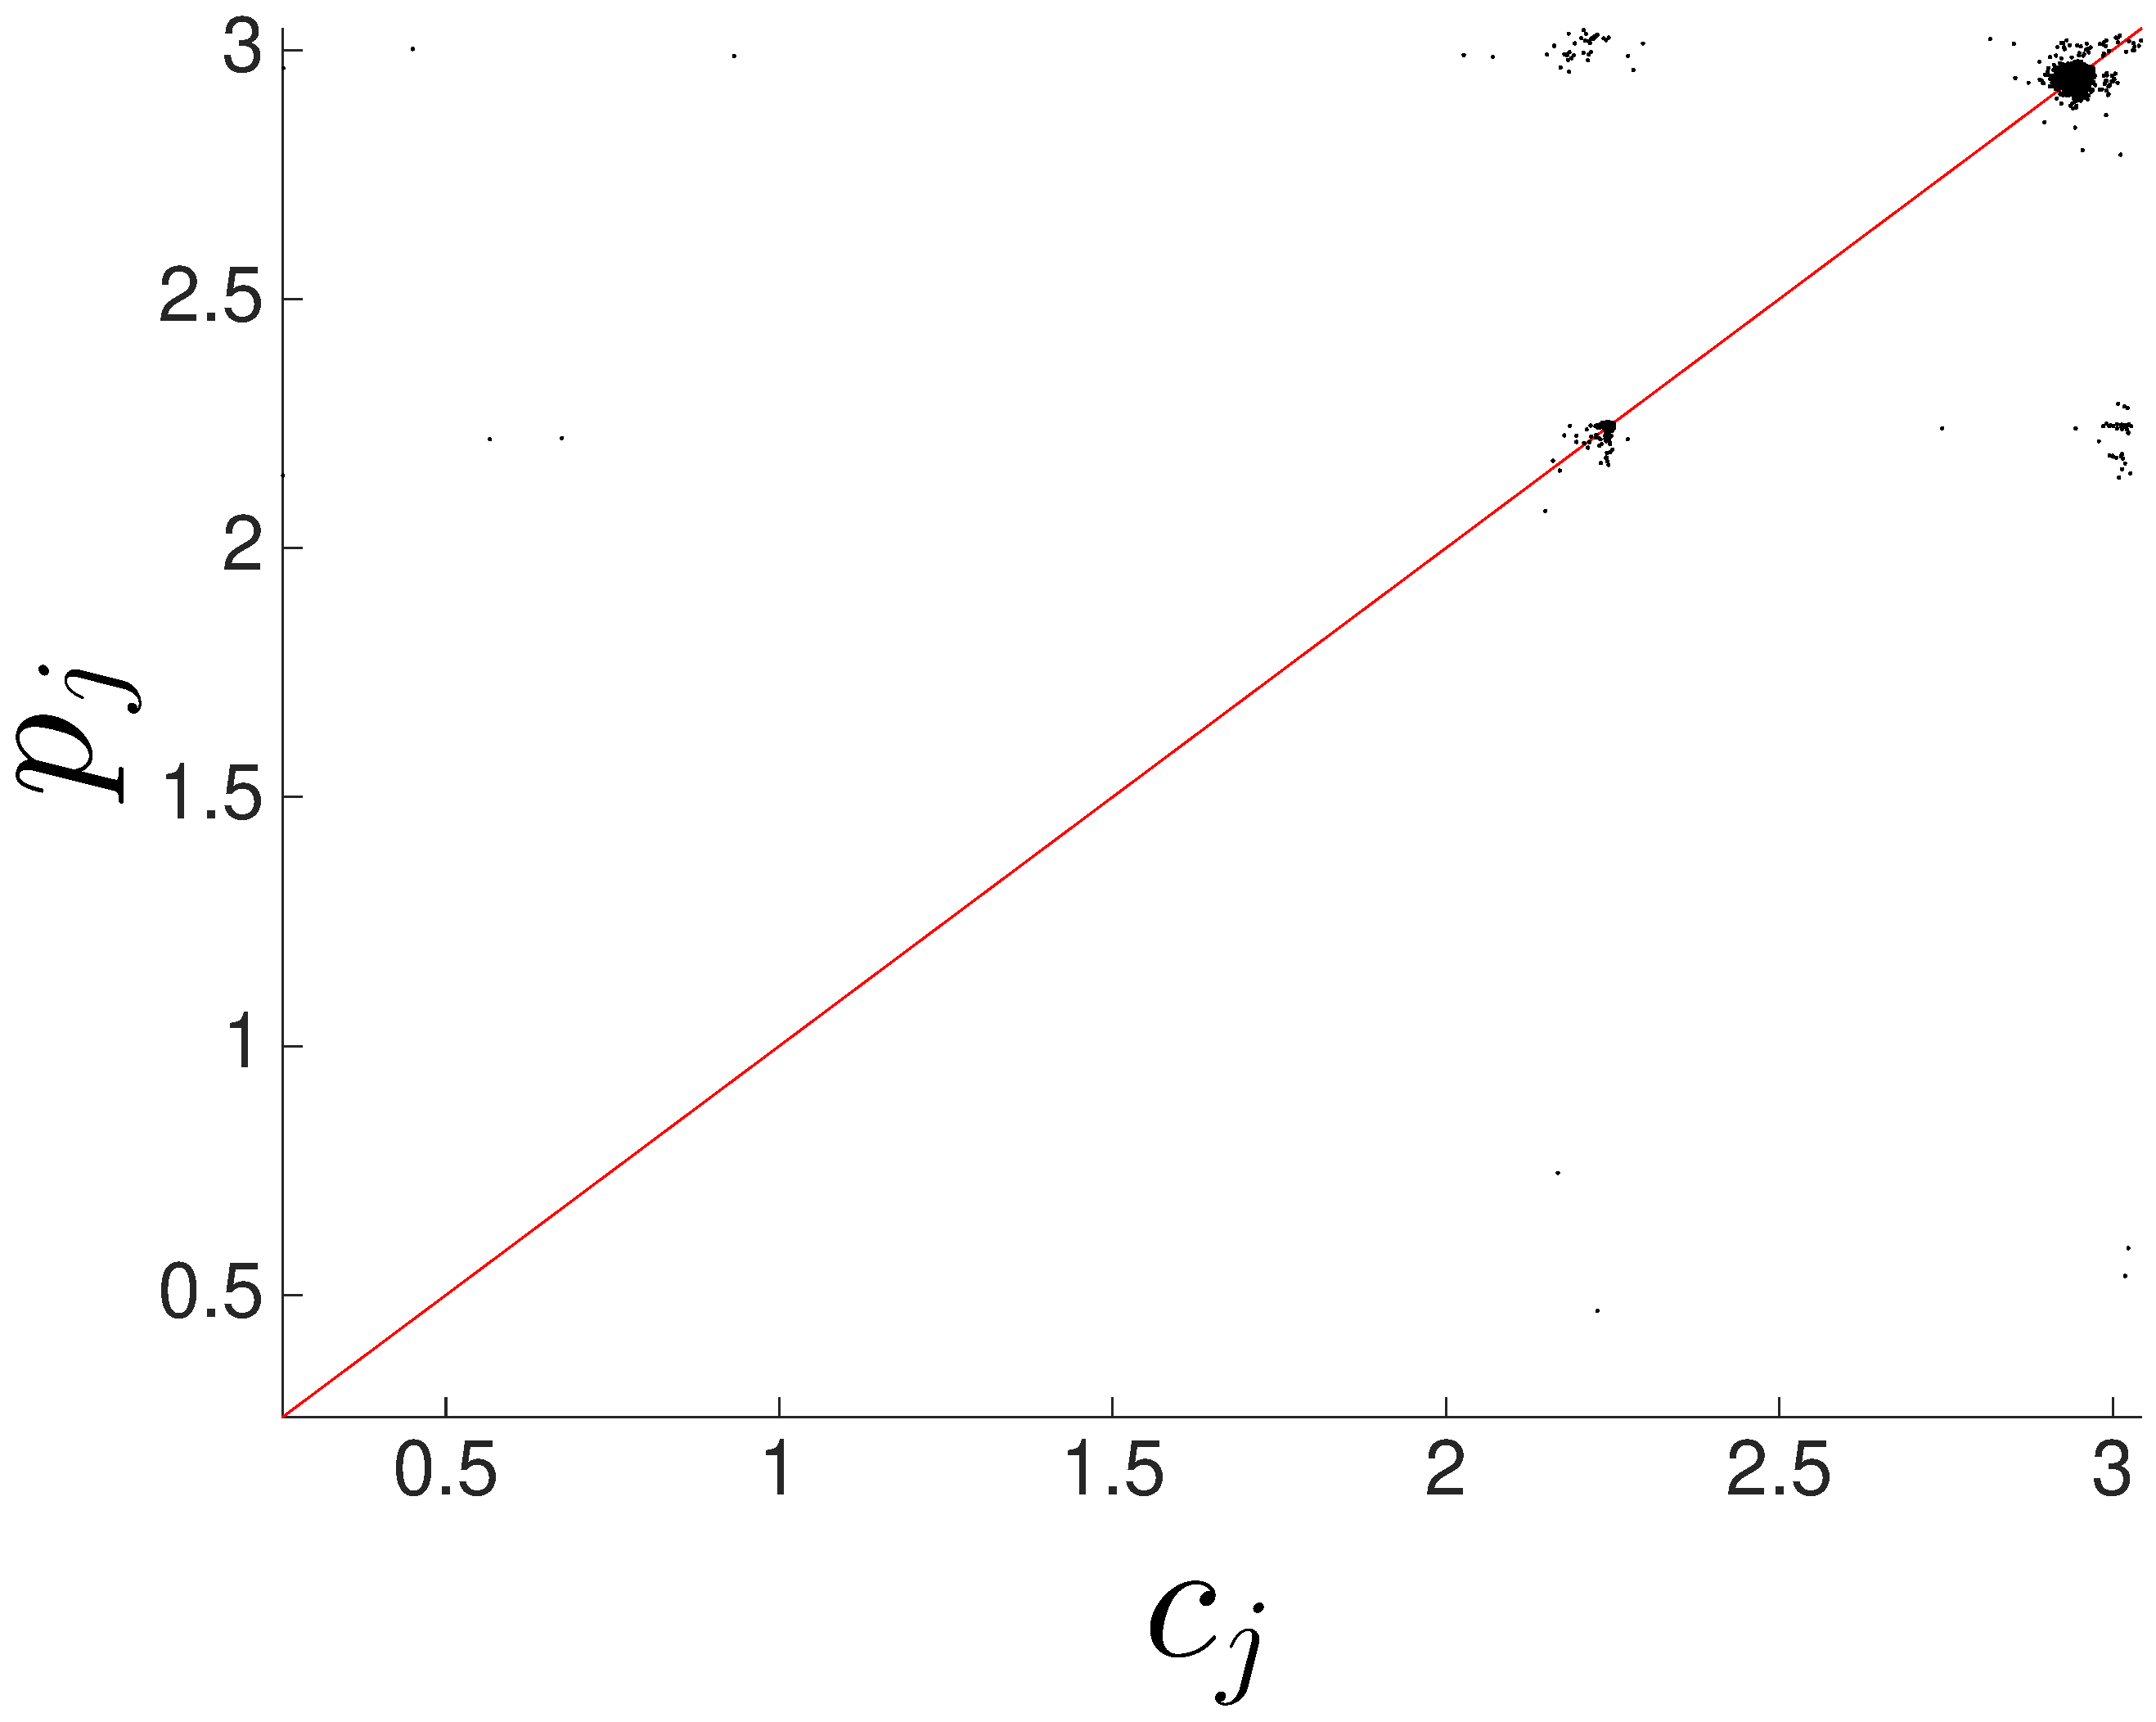
\includegraphics[width=0.6\columnwidth]{figs/svdfiveARIMAForecast} \\
    \rotatebox{90}{\large LMA} &
    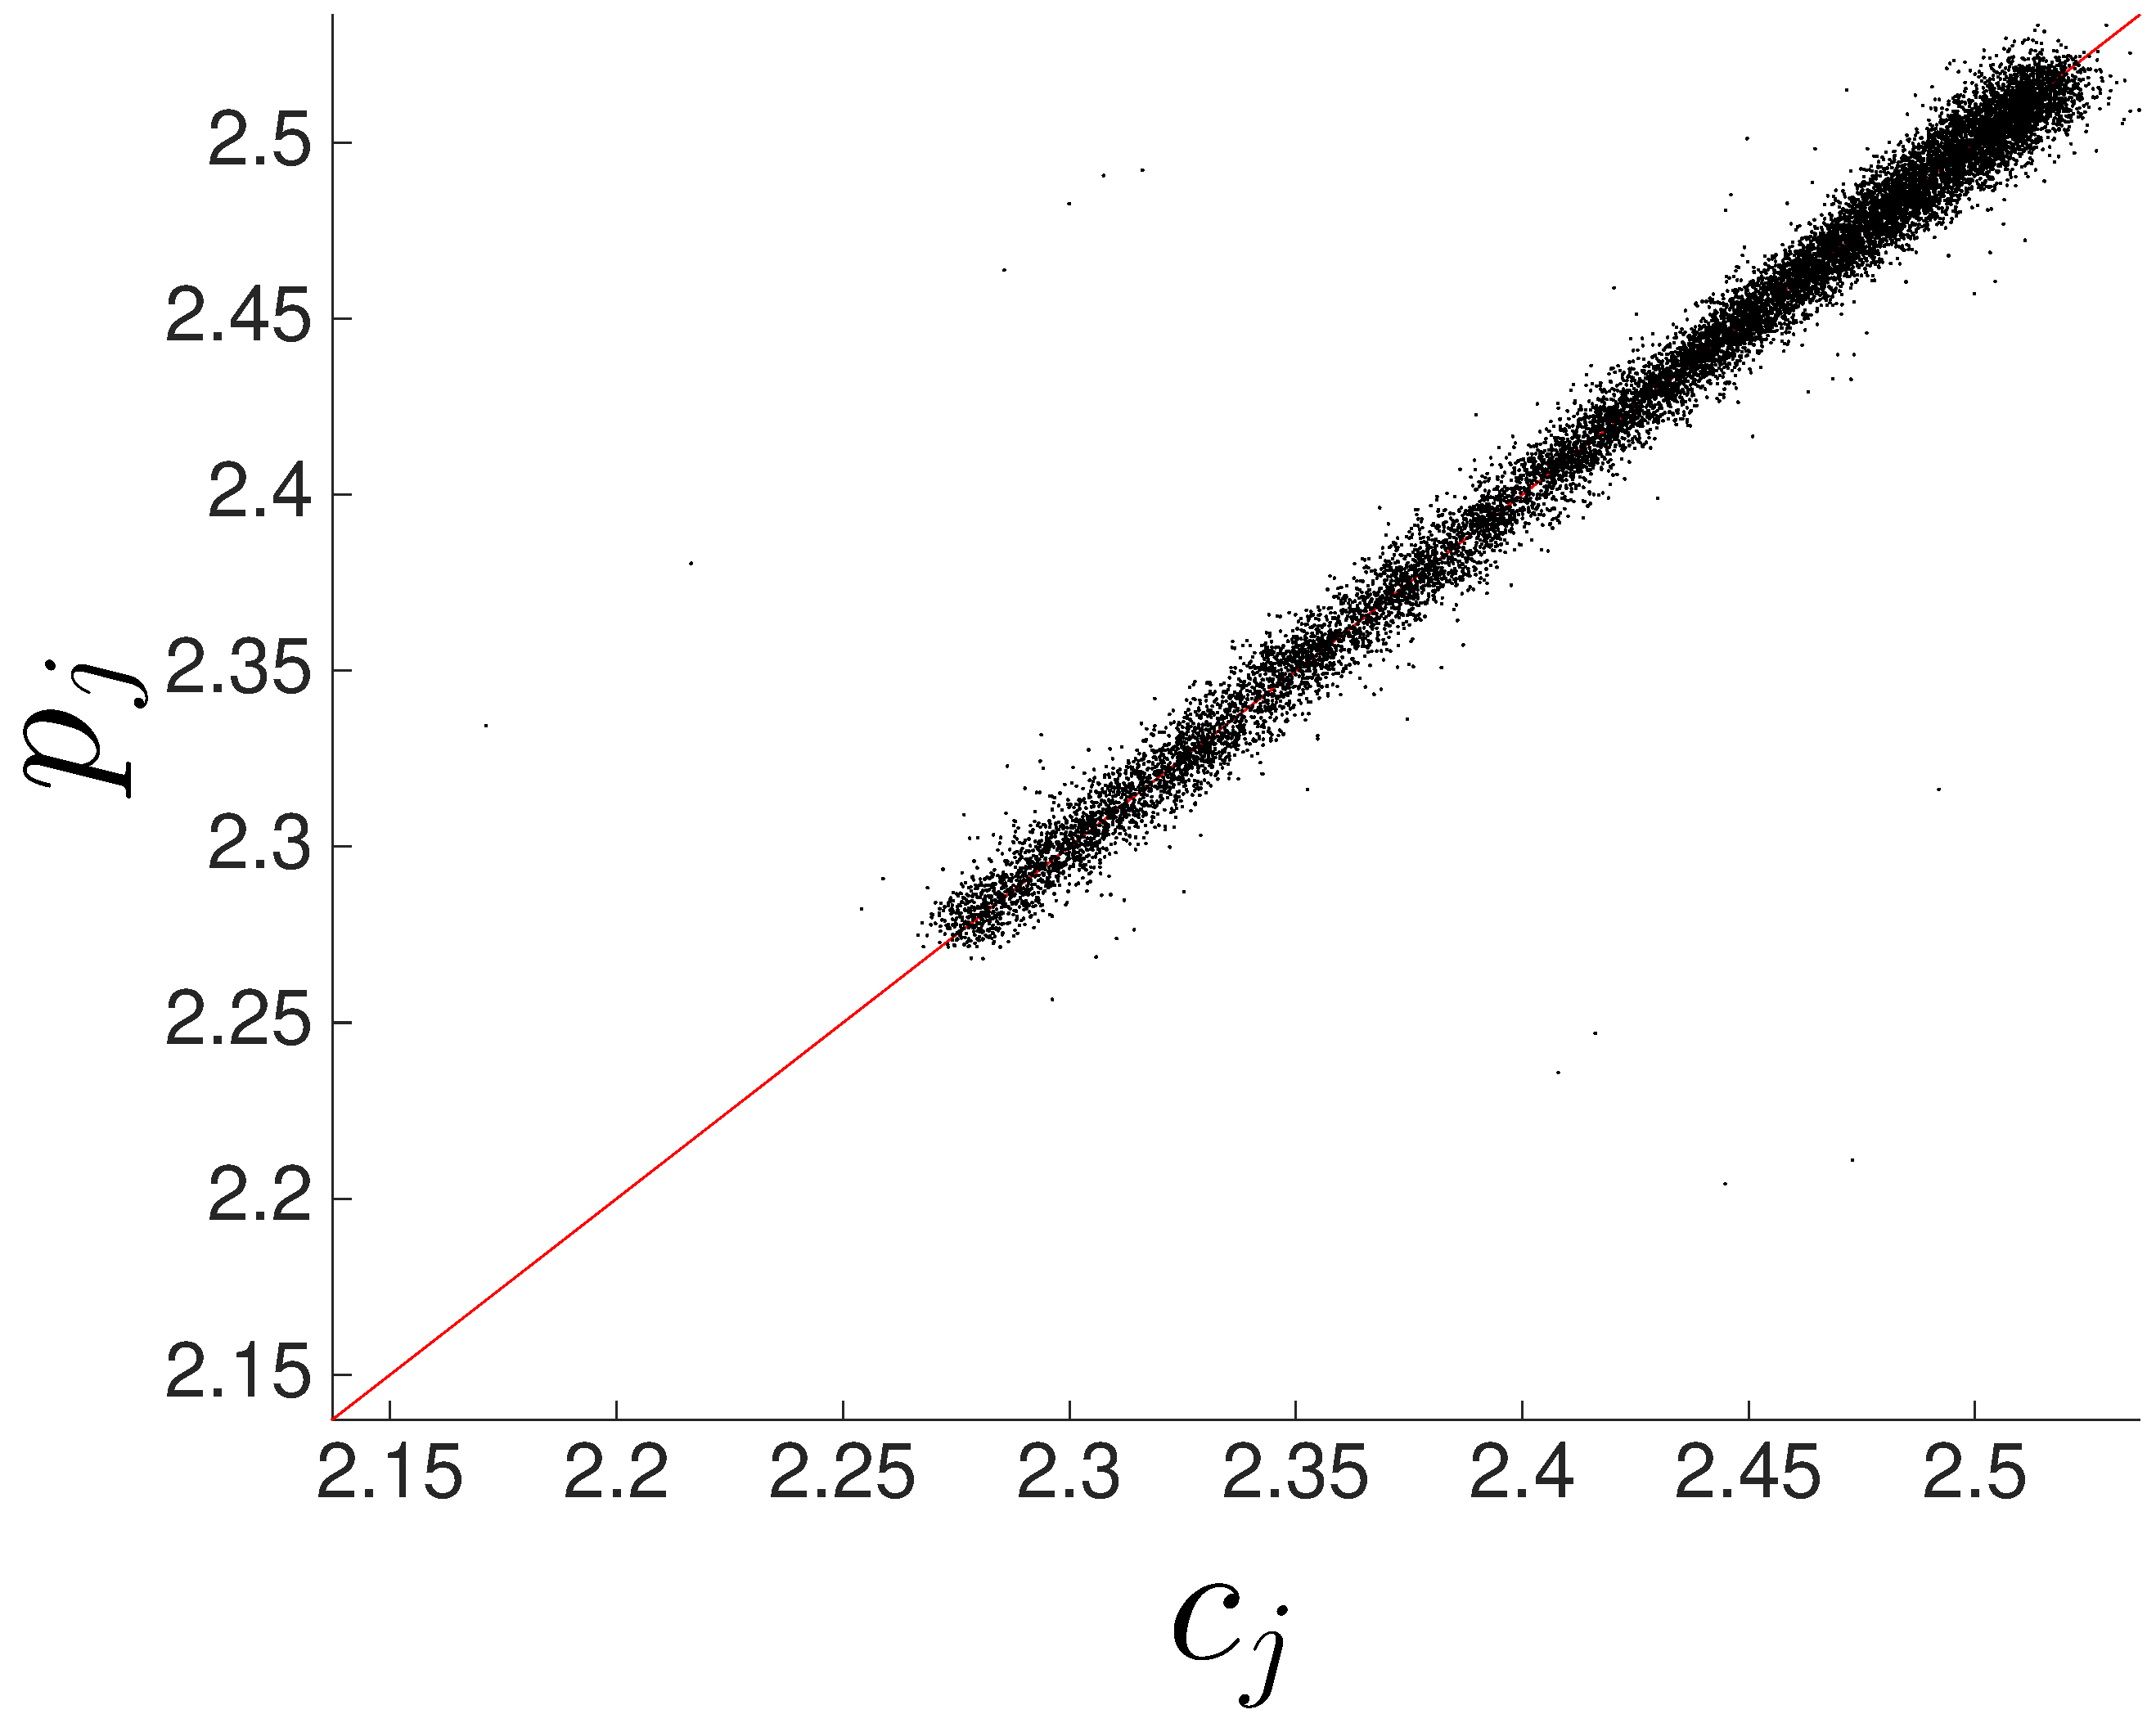
\includegraphics[width=0.6\columnwidth]{figs/colLMAForecast} &
    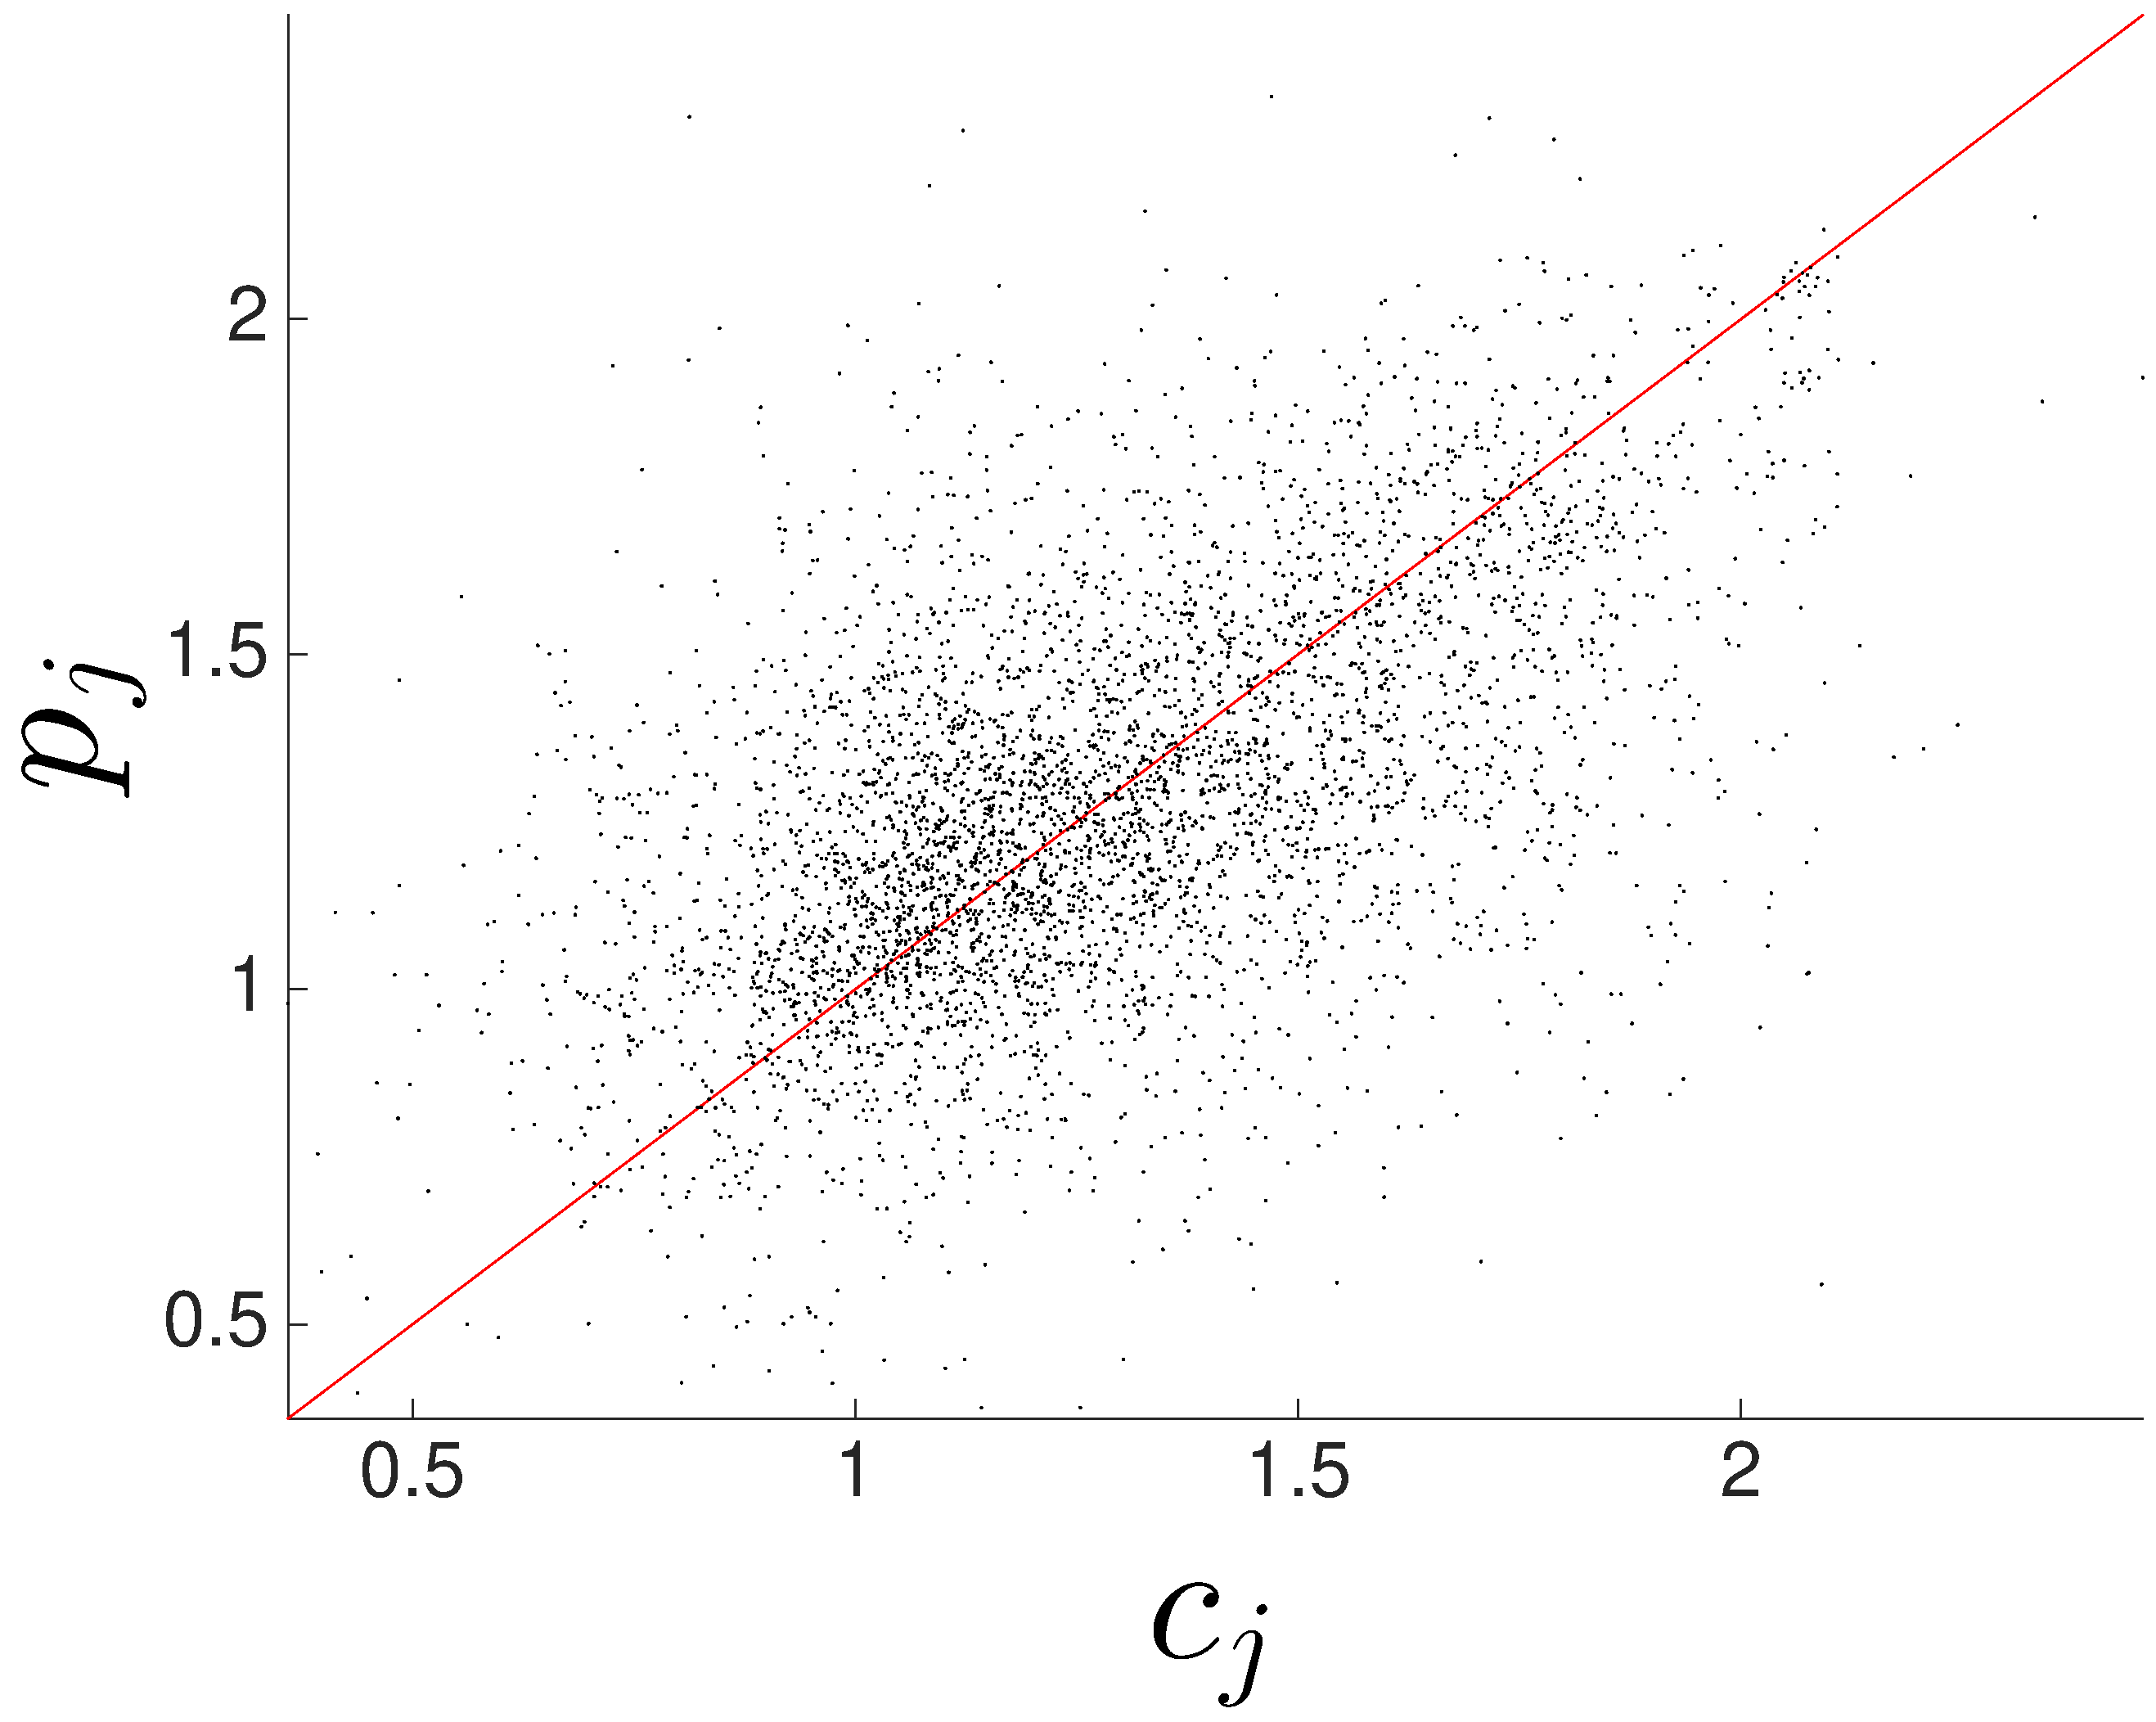
\includegraphics[width=0.6\columnwidth]{figs/gccLMAForecast} &
    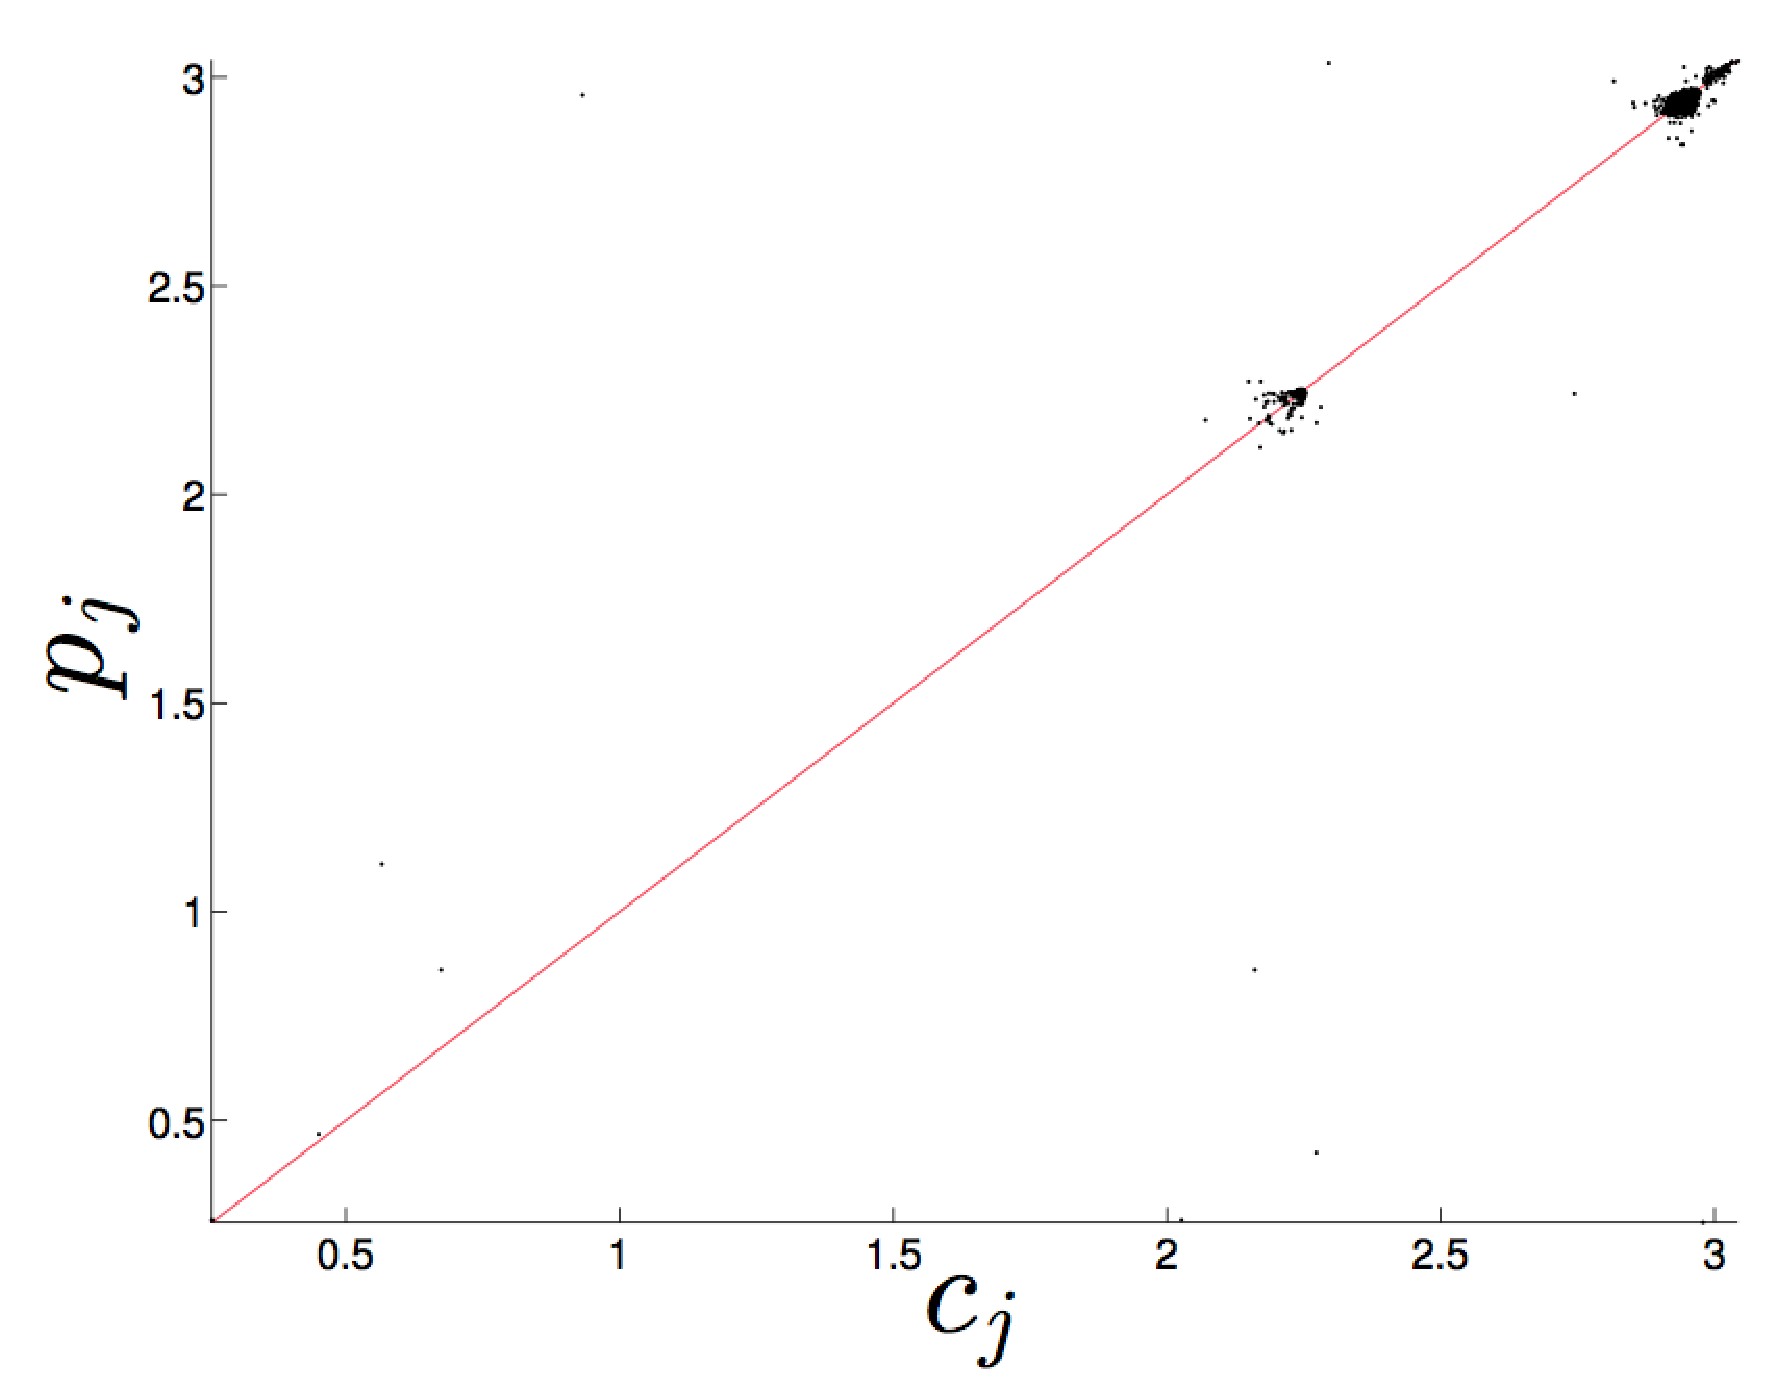
\includegraphics[width=0.6\columnwidth]{figs/svdfiveLMAForecast}
  \end{tabular}
  \caption{Predicted ($p_j$) versus true values ($c_j$) for forecasts
    of \col, \gcc, and \svdfive made using each of the four 
    strategies studied here.  }
  \label{fig:forecast-example}
\end{figure*}
In these images, the vertical axis is the prediction $p_j$ and the
horizontal axis is the true continuation $c_j$.  On such a plot, a
perfect prediction would lie on the diagonal.  LMA, for instance,
generates a very accurate prediction of the \col data, while \arima
does not.  Horizontal lines result when a constant predictor like the
\naive ~method is used on a non-constant signal.  Point clouds reflect
the structure of the distribution of the errors---roughly normally
distributed, for example, in the case of LMA on \gcc.  Note that the
shapes of some of the plots in Figure~\ref{fig:forecast-example}
(e.g., random walk and \arima on \col) are reminiscent of the
projected embedding in Figure~\ref{fig:embedding}(a).  Indeed, for a
random-walk predictor, a $p_j$ vs. $c_j$ plot is technically
equivalent to a two-dimensional embedding with $\tau=1$.  For \arima,
the correspondence is not quite as simple, since the $p_j$ values are
linear combinations of a number of past values of the $c_j$, but the
effect is largely the same\footnote{The temporal \emph{ordering} of
  the points on the \arima $p_j$ vs. $c_j$ plot does not match that of
  a projected embedding of the time series, however.}.

As a numerical measure of prediction accurary, we calculate the mean
absolute scaled error (MASE) between the true and predicted signals:
%
$$MASE = \sum_{j=n+1}^{k+n+1}\frac{|p_j-c_j|
}{\frac{k}{n-1}\sum^n_{i=2}|x_{i}-x_{i-1}|}$$
%
This error metric was introduced in \cite{MASE} as a ``generally
applicable measurement of forecast accuracy without the problems seen
in the other measurements."  Like many error metrics, MASE is a
normalized measure: the scaling term in the denominator
%
% of the MASE value
% $$\frac{1}{n-1}\sum^n_{i=2}|X_{i,obs}-X_{i-1,obs}|$$
%
is the average in-sample forecast error for a random-walk prediction
over the initial training signal $\{x_i\}^n_{i=1}$.  That is, MASE$<1$
means that the prediction error in question was, on the average,
smaller than the average error of a random-walk forecast on the
training data.  Analogously, MASE$>1$ means that the corresponding
prediction method did \emph{worse}, on average, than the random-walk
method.  While its comparative nature is somewhat different than
traditional metrics like normalized root mean squared error, MASE has
the significant advantage of allowing one to make a fair comparison
across varying methods, prediction horizons, and signal
scales---attributes that are key to any broad study of predictability.

MASE scores for all 360 experiments are tabulated in the four middle
columns in Table~\ref{tab:error}.
%\begin{table*}
%\caption{Mean absolute scaled error (MASE) scores and weighted
%  permutation entropies for all eight processes studied in this paper.
%  LMA $=$ Lorenz method of analogues; RW $=$ random-walk prediction.
%  \alert{please reorder the columns from left to right to match the
%    order in which the methods were introduced, rather than in the
%    reverse of that order}}
%  \begin{center}
%  \begin{tabular*}{\textwidth}{@{\extracolsep{\fill} } cccccc}
%  \hline\hline Signal & LMA MASE & \arima MASE & na\"{i}ve MASE & RW MASE & WPE \\
%  \hline
%
%  \col       & $0.050 \pm 0.002$ & $0.599 \pm 0.211$ & $0.571 \pm 0.002$  & $1.001 \pm 0.002$ & $0.513 \pm 0.003$ \\
%
%  \gcc       & $1.530 \pm 0.021$ & $1.837 \pm 0.016$ & $1.797 \pm 0.010$  & $1.138 \pm 0.011$ & $0.943 \pm 0.001$ \\
%
%  \svdone    & $0.827 \pm 0.076$ & $0.714 \pm 0.075$ & $2.676 \pm 4.328$  & $0.933 \pm 0.095$ & $0.957 \pm 0.016$ \\
%
%  \svdtwo    & $1.279 \pm 0.020$ & $2.163 \pm 0.027$ & $3.054 \pm 0.040$  & $1.125 \pm 0.012$ & $0.846 \pm 0.004$ \\
%
%  \svdthree  & $0.619 \pm 0.021$ & $0.713 \pm 0.010$ & $31.386 \pm 0.282$ & $0.707 \pm 0.009$ & $0.716 \pm 0.006$ \\
%
%  \svdfour   & $0.779 \pm 0.036$ & $0.979 \pm 0.032$ & $2.661 \pm 0.074$  & $1.034 \pm 0.035$ & $0.825 \pm 0.008$ \\
%
%  \svdfive   & $0.718 \pm 0.048$ & $2.370 \pm 0.051$ & $20.870 \pm 0.192$ & $1.001 \pm 0.047$ & $0.678 \pm 0.007$ \\
%
%  \svdsix    & $0.739 \pm 0.068$ & $1.438 \pm 0.061$ & $2.197 \pm 0.083$  & $1.060 \pm 0.055$ & $0.748 \pm 0.011$ \\
%
%  \hline\hline
%  \end{tabular*}
%  \end{center}
% \label{tab:error}
%  \end{table*}%
%  
 \begin{table*}
\caption{Mean absolute scaled error (MASE) scores and weighted
  permutation entropies for all eight processes studied in this paper.
  LMA $=$ Lorenz method of analogues; RW $=$ random-walk prediction.
  }
  \begin{center}
  \begin{tabular*}{\textwidth}{@{\extracolsep{\fill} } cccccc}
  \hline\hline 
Signal & RW MASE & na\"{i}ve MASE & \arima MASE & LMA MASE & WPE \\
\hline
  \col       & $1.001 \pm 0.002$ & $0.571 \pm 0.002$  & $0.599 \pm 0.211$ & $0.050 \pm 0.002$ & $0.513 \pm 0.003$ \\
  \gcc       & $1.138 \pm 0.011$ & $1.797 \pm 0.010$  & $1.837 \pm 0.016$ & $1.530 \pm 0.021$ & $0.943 \pm 0.001$ \\
  \svdone    & $0.933 \pm 0.095$ & $2.676 \pm 4.328$  & $0.714 \pm 0.075$ & $0.827 \pm 0.076$ & $0.957 \pm 0.016$ \\
  \svdtwo    & $1.125 \pm 0.012$ & $3.054 \pm 0.040$  & $2.163 \pm 0.027$ & $1.279 \pm 0.020$ & $0.846 \pm 0.004$ \\
  \svdthree  & $0.707 \pm 0.009$ & $31.386 \pm 0.282$ & $0.713 \pm 0.010$ & $0.619 \pm 0.021$ & $0.716 \pm 0.006$ \\
  \svdfour   & $1.034 \pm 0.035$ & $2.661 \pm 0.074$  & $0.979 \pm 0.032$ & $0.779 \pm 0.036$ & $0.825 \pm 0.008$ \\
  \svdfive   & $1.001 \pm 0.047$ & $20.870 \pm 0.192$ & $2.370 \pm 0.051$ & $0.718 \pm 0.048$ & $0.678 \pm 0.007$ \\
  \svdsix    & $1.060 \pm 0.055$ & $2.197 \pm 0.083$  & $1.438 \pm 0.061$ & $0.739 \pm 0.068$ & $0.748 \pm 0.011$ \\  
    \hline\hline
  \end{tabular*}
  \end{center}
 \label{tab:error}
  \end{table*}%
  
  
  
  
In view of the discussion at the end of the previous paragraph, the
fact that the values in the second-from-left column are not
identically equal to 1.00 may be somewhat surprising.  This can happen
due to differences between in-sample and out-of-sample forecasting;
the last 10\% of \svdthree, for instance---the out-of-sample
signal---was more amenable to random-walk prediction, on the average,
than the first 90\%.  See Section~\ref{sec:results} for a deeper
discussion of this effect.

Comparing the values in Table~\ref{tab:error} with the geometry of the
plots in Figure~\ref{fig:forecast-example}, one can see some obvious
correspondences.  The average LMA MASE score for the \col signals was
$0.050$, for instance, while \arima scored much worse ($0.599$).  That
is, LMA performed roughly 20 times better on \col signals than a
random-walk predictor, while \arima only outperformed random walk by a
factor of 1.7.  This is in accordance with the visual appearance of
the corresponding images in Figure~\ref{fig:forecast-example}.  

In other cases, the correspondence between MASE score and the visual
appearance of these kinds of plots is not so clear cut.  The plots of
LMA predictions of \col and \svdfive both lie near the diagonal, for
instance, but the corresponding MASE scores were very different:
$0.050$ for \col and $0.718$ for \svdfive (resp., 20 and 1.4 times
better than random-walk forecasts of the same signals).  This is a
result of the normalization in the MASE score calculation.  Recall
from Section~\ref{sec:simple} that the random-walk method performs
especially poorly on signals that oscillate rapidly.  \col fits this
description, so the random-walk error on this signal---the denominator
of the four MASE scores in the first row of the Table---is
pathologically high, which skews those scores down.  Random-walk
prediction is very effective for the \svdfive signal, on the other
hand, so the denominator is small and the MASE scores are skewed
upwards.  

Normalization is, as is often the case, a double-edged sword.  Here,
it facilitates comparisons across signals of different types and
lengths, but its particular pathologies must be taken into account
when analyzing the results, as discussed at more length in
Section~\ref{sec:results}.

% Table \ref{tab:error} provides the MASE distributions
% {\color{red}[Joshua: Ryan, Is this the right word? we give mean $\pm$
%       std. dev but some have very skewed right tails]} for each of
% the eight signals and three prediction strategies, these are averaged
% over 15 runs of each signal-method combination. For later comparison,
% Table \ref{tab:error} also has the complexity measure we introduce in
% Section \ref{sec:meaComplex}.

%[and cherry pick a few examples of \gcc and \col to put in the text ]


%---works quite well on the trace in Figure~%\ref{fig:ipc}, as%
%shown in Figure~\ref{fig:lmacol}.
%
%\begin{figure}
%   \centering
%\begin{subfigure}{\columnwidth}
%    \includegraphics[width=\columnwidth]{%colPredShortTS}
%    \caption{\col }
%    \label{fig:lmacol}
%  \end{subfigure}%
%
%    \begin{subfigure}{\columnwidth}
%    \includegraphics[width=\columnwidth]{%colPredShortTS}
%    \caption{\gcc}
%    \label{fig:lmagcc}
%  \end{subfigure}
%  \begin{subfigure}{\columnwidth}
%%    \includegraphics[width=\columnwidth]{%colPredShortTS}
%    \caption{\svdfive}
%    \label{fig:lmasvdfive}
%  \end{subfigure}%
%  \caption{{\color{red} [If Liz thinks we should %include these I actually need to generate this %figure]}An LMA-based forecast of
%       processor-efficiency performance trace from the%\col ,\gcc and \svdfive generating processes.  Red %circles and blue $\times$s are the true and
%       predicted values, respectively; vertical bars %show where these
%       values differ.}\label{fig:lmapredictions}
% \end{figure}
%
%\begin{figure}[htbp]
%  \centering
%   \includegraphics[width=\textwidth]{colPredShortTS}
%    \caption{A forecast of the last 4,000 points of the %signal in
%      Figure~\ref{fig:ipc} using an LMA-based strategy on %the
%      embedding in Figure~\ref{fig:embedding}.  Red circles %and blue
%      $\times$s are the true and predicted values, %respectively;
%      vertical bars show where these values differ.}
%\label{fig:lmacol}
%\end{figure}
%
%\begin{figure}[htbp]
%  \centering
%    \includegraphics[width=\textwidth]{colPredShortTS}
%     \caption{{\color{red} [actually need to generate this %figure]}An LMA-based forecast of the last 4,000 points of a
%       processor-load performance trace from the \gcc
%       benchmark.  Red circles and blue $\times$s are the %true and
%       predicted values, respectively; vertical bars show %where these
%       values differ.}
%\label{fig:lmagcc}
%\end{figure}
%
%On the other hand, if we use the same approach to %forecast the
%processor efficiency (IPC) of the \gcc time series, %the
%prediction is far less accurate; see Figure~%\ref{fig:lmagcc}.
%Figure~\ref{fig:lmasvdfive} is clearly a better %prediction than Figure~\ref{fig:gccLMA} but not nearly as good as the \col forecast.


%This gets at the utility of the contribution of this %paper: These time series all come from the same system---computers---but they are not equally predictable (at this point by LMA). For a practitioner is it the case that
%  Our
%conjecture is that while they come from similar systems \gcc produces processor load traces on the top of the complexity spectrum whereas \col produces processor loads with complexity in the mid to low region of the complexity spectrum. If this is the case then \gcc might be much better predicted using a method like Random Walk or \naive which can effectively predict in the presence of complexity. This is explored more rigorously in the results Section of this paper (Section \ref{sec:results}. So that we don't have to compare the forecast accuarcy by visual comparing the predictions we calculate a figure of merit to compare the predictions.






\section{Measuring Structural Complexity }\label{sec:meaComplex}
{\color{red} NOT EDITABLE}

THINGS TO DO
\begin{enumerate}
\item rewrite for consistency in notation. For example, some parts of the paper call word length $l$ and some call it $n$.

\item make sure it is clear and we justify that detecting and characterizing structural complexity is hard for real-valued noisy time series.
\item Quantifying structured and unstructured complexity is nontrivial in the case of real-valued noisy time series but WPE does this. [[talk about again here but justify in information theory section]]
\item justify and explain the regime split in \svd {\color{red} I(joshua) moved this justification in the experimental methods section, it just needs to be explored here by applying windowed wpe and explaining that method}
\end{enumerate}


For the purposes of this paper, one can view entropy as a measure of complexity
and predictability in a time series.  A high-entropy time series is almost
completely unpredictable---and conversely.  This can be made more rigorous:
Pesin's relation \cite{pesin77} states that in chaotic dynamical systems, the
Shannon entropy rate is equal to the sum of the positive Lyapunov exponents,
$\lambda_i$. The Lyapunov exponents directly quantify the rate at which nearby
states of the system will diverge with time: $\left| \Delta x(t) \right| \approx
e^{\lambda t} \left| \Delta x(0) \right|$.  The faster the divergence, the more
difficult prediction becomes.

Utilizing entropy as a measure of temporal complexity is by no means a new idea
\cite{Shannon1951, mantegna1994linguistic}.  Its effective usage requires
categorical data: $x_t \in \mathcal{S}$ for some finite or countably infinite
\emph{alphabet} $\mathcal{S}$, whereas data taken from real-world systems is
effectively real-valued.  To get around this, one must discretize the data---
typically achieved by binning.  Unfortunately, this is rarely a good solution to
the problem, as the binning of the values introduces an additional dynamic on
top of the intrinsic dynamics whose entropy is desired.  The field of symbolic
dynamics studies how to discretize a time series in such a way that the
intrinsic behavior is not perverted, but these methods are fragile in the face
of noise and require further understanding of the underlying system, which
defeats the purpose of measuring the entropy in the first place.

Bandt and Pompe introduced the \emph{permutation entropy} (PE) as a ``natural
complexity measure for time series" \cite{bandt2002per}.  Permutation entropy
employs a method of discretizing real-valued time series that follows the
intrinsic behavior of the system under examination.  Rather than looking at the
statistics of sequences of values, as is done when computing the Shannon
entropy, permutation entropy looks at the statistics of the \emph{orderings} of
sequences of values using ordinal analysis. Ordinal analysis of a time series is
the process of mapping successive time-ordered elements of a time series to
their value-ordered permutation of the same size.  By way of example, if $(x_1,
x_2, x_3) = (9, 1, 7)$ then its \emph{ordinal pattern}, $\phi(x_1, x_2, x_3)$,
is $231$ since $x_2 \leq x_3 \leq x_1$.  This method has many features; among
other things, it is generally robust to observational noise and requires no
knowledge of the underlying mechanisms.

\begin{mydef}[Permutation Entropy]

  Given a time series $\{x_t\}_{t = 1,\dots,T}$. Define $\mathcal{S}_n$ as all
  $n!$ permutations $\pi$ of order $n$. For each $\pi \in \mathcal{S}_n$ we
  determine the relative frequency of that permutation occurring in $\{x_t\}_{t
  = 1,\dots,T}$:
  \begin{align*}
    p(\pi) = \frac{\left|\{t|t \leq T-n,\phi(x_{t+1},\dots,x_{t+n}) = \pi\}\right|}{T-n+1}
  \end{align*}
  Where $|\cdot|$ is set cardinality. The \emph{permutation entropy} of order $n
  \ge 2$ is defined as
  \begin{align*}
  H(n) = - \sum_{\pi \in \mathcal{S}_n} p(\pi) \log_2 p(\pi)
  \end{align*}

\end{mydef}

Notice that $0\le H(n) \le \log_2(n!)$ \cite{bandt2002per}.  With this in mind,
it is common in the literature to normalize permutation entropy as follows:
$\frac{H(n)}{\log_2(n!)}$.  With this convention, ``low'' entropy is close to 0
and ``high'' entropy is close to 1. Finally, it should be noted that the
permutation entropy has been shown to be identical to the Shannon entropy for {\color{red}[[Ryan is this the case or is it the KS entropy?]]}
many large classes of systems \cite{amigo2012permutation}.

Here we will be utilizing a variation of the permutation entropy, the
\emph{weighted permutation entropy} (WPE)~\cite{fadlallah2013}. The weighted
permutation entropy attempts to correct for observational noise which is larger
than some trends in the data, but smaller than the larger scale features --- for
example, a signal that switches between two fixed points with noise about those
fixed points. The weighted permutation entropy would be dominated by the
switching rather than by the stochastic fluctuation. To accomplish this, the
\emph{weight} of a permutation is taken into account:
\begin{align*}
  w(x_{t+1:t+n}) = \frac{1}{n}
                 \sum_{x_i \in \{x_{t+1:t+n}\}}
                 \left( x_i - \bar{x}_{t+1:t+n} \right)^2
\end{align*}
where $x_{t+1:t+n}$ is a sequence of values $x_{t+1}, \ldots, x_{t+n}$, and
$\bar{x}_{t+1:t+n}$ is the arithmetic mean of those values.

The weighted probability of a permutation is then:
\begin{align*}
  p_w(\pi) = \frac{\displaystyle \sum_{t \le T - n} w(x_{t+1:t+n}) \cdot \delta(\phi(x_{t:t+n}), \pi) }{\displaystyle \sum_{t \le T - n} w(x_{t+1:t+n})}
\end{align*}
where $\delta(x, y)$ is 1 if $x = y$ and 0 otherwise. Effectively, this weighted
probability enhances permutations involved in ``large'' features and demotes
permutations which are small in amplitude relative to the features of the time
series. The weighted permutation entropy is then:
\begin{align*}
  H_w(n) = - \sum_{\pi \in \mathcal{S}_n} p_w(\pi) \log_2 p_w(\pi),
\end{align*}
which can also be normalized by dividing by $\log_2(n!)$, and will be in all the
results of this paper.

In practice, calculating permutation entropy and weighted permutation entropy
involves choosing a good value for the word length $n$. The primary
consideration is that the value be large enough that forbidden ordinals are
discovered, yet small enough that reasonable statistics over the ordinals are
gathered: e.g.:
\begin{align*}
  n = \operatornamewithlimits{argmax}_\ell \{ T \gtrapprox 100 \ell! \},
\end{align*}
assuming an average of 100 counts per ordinal is sufficient. In the literature,
$3 \le n \le 6$ is a standard choice --- generally without any formal
justification. In theory, the permutation entropy should reach an asymptote with
increasing $n$, but that requires an arbitrarily long time series. In practice,
what one should do is calculate the \emph{persistent} permutation entropy by
increasing $n$ until the result converges, but data length issues can intrude
before that convergence is reached.

\subsection{Regime Selection:Detecting complexity shift in a time series}\label{sec:wpeRegime}

{\color{red} this is from a previous paper I wrote, if this is used we need to update the plots to use wpe and windowed wpe instead of standard pe, also not sure how much of this is necessary but added as starting point}

Permutation entropy is a measure of the complexity of time series as a whole, but it can also be used to calculate a dynamical shift in a time series as illustrated in \cite{cao2004det}. To detect dynamical changes in a time series we follow the methods of \cite{cao2004det}. Partition the time series  $\{x_t\}_{t = 1,\dots,T}$ into overlapping\footnote{Following \cite{cao2004det} we use maximal overlapping block. (A window shift of 1.)} (or nonoverlapping) blocks. Calculate $H(n)$ for each block, and treat $H(n)$ as a function of time.  According to \cite{cao2004det} drastic changes in permutation entropy can indicate change in the underlying model.

In addition to introducing this block method, \cite{cao2004det} introduce the use of a \emph{lag} when calculating permutation entropy. This is identical to the lag used in delay coordinate embedding and often the same language is used. Cao et al. describe the process of symbolization in \cite{bandt2002per} as embedding the time series in an $m$ dimensional symbol space. When we symbolize a scalar time series,$\{x_t\}_{t = 1,\dots,T}$, we first embed the scalar time series into $m$ dimensional vectors before matching this to a symbol in $\mathcal{S}_m$. So pre-symbolization our time series changes from scalar to objects of the form:  $$[x(i),\,x(i+1),\,\dots,x(i+(m-1)]$$ This vector is then mapped by $\phi$ to a symbol in $\mathcal{S}_m$. Cao et al. argue that we can view this as embedding the time series in an $m$ dimensional space with lag 1. Cao et al. then state ``Since in practice the optimal $L$[lag] may be different from 1, we shall present the idea for any $m$[embedding dimension] and $L$."\footnote{No further explanation is given about why this is the case.} To not confuse notation we define $\tau$ to be the lag parameter. The process of symbolization then starts with transforming the scalar time series into a set of vectors of the form $$[x(i),\,x(i+\tau),\,\dots,x(i+(m-1)\tau]$$ where $\tau\ge1$.

\subsubsection{Example: Concatenated Time Series}\label{sec:concatenate}
As an example of this detection, consider Figure \ref{fig:ts-banded} (a). This is a plot of a concatenated time series comprised of several orbits of the Logistic map with varying parameters as well as intermittent noise. Each concatenated band (either an orbit of the Logistic map or noise) is 50,000 points. The bands of noise are generated with Matlab's \verb|randsample|, using the chaotic bands as the sampling population. Each Logistic map trajectory begins at $x=0.6$. The period-two trajectories have an $R$ of 3.2, the period-three trajectory has an R of 3.838, and the chaotic trajectories have an $R$ of 3.65.

The concatenated time series is comprised of two period-two trajectories($t=0-50,000$ and $t=250,000-300,000$), one period-three trajectory($t=100,000-150,000$), two chaotic trajectories ($t=50,000-100,000$ and $t=200,000-250,000$, and two different bands of noise($t=150,000-200,000$ and $t=300,000-350,000$). Visually the bands of noise and the chaotic trajectory are indistinguishable. If this were an observed time series from a real process, it would be impossible to visually identify which bands were generated deterministically and which were simply noise. If we calculate block permutation entropy as discussed in \cite{cao2004det} and plot this as a function of time it becomes very clear which bands have structure and which do not.

In Figure \ref{fig:ts-banded} (b) we plot the concatenated time series, as well as permutation entropy as a function of time(red, blue and green curves). The red, blue and green curves are the permutation entropy calculated using $m=5$ and $\tau = 1,2,3$ (respectively). Using these curves it is clear that bands 2 and 5 ($t=50,000-100,000$ and $t=200,000-250,000$) are chaotic because they have structure\footnote{Permutation entropy less than one.}. On the other hand, bands 4 and 7 ($t=150,000-200,000$ and $t=300,000-350,000$) have no structure\footnote{Permutation entropy of one.} and are the noise bands. This is in fact the case when comparing to the way the time series was constructed.

The main advantage we can see to the use of lags other than 1 is for analysis of periodicity. This is also the major advantage listed in \cite{cao2004det}. Notice in the period 2 bands the blue curve (permutation entropy calculated with a lag of 2) is zero. This means that with a lag of 2 the period 2 orbit is perfectly structured\footnote{Equivalently, not enough permutations are being realized to impact the calculation of $H(n)$}. If we increase the lag to 3 (the green curve) the two period-two bands have a little bit of structure(as some permutations will be realized) but the period 3 band has zero permutation entropy.

%TSLogistic = [period2Logistic;chaosLogistic;period3Logistic;randomSampleFromMap2;chaosLogistic;period2Logistic;randomSampleFromMap3];

%\begin{figure}
%  \centering
%  \subfigure{\includegraphics[width=\columnwidth]{unused-figs/ts-banded-alone}}
%    {(a)}
%
%  \subfigure{\includegraphics[width=\columnwidth]{unused-figs/ts-banded-pe}}
%  {(b)}
%  \caption{ (a) The concatenated time series discussed in Section~\ref{sec:concatenate}. (b) Plot of the concatenated time series from Section~\ref{sec:concatenate}, as well as permutation entropy as a function of time(blue,green and red curves). Each permutation entropy curve shown is calculated using $m=5$, however, the red,blue and green curve use a $\tau = 1,2,3$ respectively.}\label{fig:ts-banded}
%\end{figure}






and what is it good for with forward pointer to the other sections



\subsubsection{Example: The transient Logistic map}
In Section~\ref{sec:concatenate} we discussed a time series which stayed in a parameter regime for long amounts of time and then abruptly changed. As we showed, permutation was a great proxy to detect this change. Another type of parameter change that may occur in a physical system is constant parameter drift, i.e., some parameter slowly changes over time. To explore this type of parameter drift we construct the same time series as was used in \cite{cao2004det}. Iterate the logistic map, starting with $R=2.8$, then at every iteration increase $R$ by $10^{-5}$ until $R=4$. The time series, which can be seen in Figure~\ref{fig:translogistic} appears very similar to the standard bifurcation diagram for the Logistic map. The curves in red and blue are the permutation entropy calculated with $m=5$ and $\tau = 1,2$ (respectively).

 As we can see, as bifurcations occur in the dynamics the permutation entropy changes as well. An interesting feature of block calculations are the spikes that occur at bifurcation points. As the block begins to encompass multiple regimes, e.g., fixed point and  period two, permutations are being realized for both regimes. This overlap causes an increase in the time series complexity, and thus a spike in the permutation entropy. The dips you see in the second half correspond to bands of periodicity which occur between the chaos. It is worth noting, that the blue curve (permutation entropy with lag 2) does not go to zero in the period 2 parameter range. This is because this is not a true period 2 orbit but transient that is moving across \emph{several} period 2 orbits, thus it maintains a higher level of complexity, albeit still very low.

 This illustrates that permutation entropy can not only distinguish between instant (and drastic) parameter shifts but also very slow and gradual parameter drift.

\begin{figure}[ht]
  \centering
  \includegraphics[width=\columnwidth]{unused-figs/tstranslog-perm}
  \caption{Transient Logistic map time series and permutation entropy curves. Both permutation entropy curves are calculated with $m=5$, the red and blue correspond to $\tau = 1,2$ respectively.}
  \label{fig:translogistic}
\end{figure}
%\begin{enumerate}
%\item do with henon bifurcation. what happens near the broken chaotic window

%\end{enumerate}


The weighted permutation entropy for the \svd program is given in
Fig.~\ref{fig:wwpe}. To generate this image a window of 5,000 values slid over
the time series. Within each of those windows, the statistics over words of
length 4 are computed and the WPE is calculated. The gray bands denote regions
where the 5,000 value window overlapped visually-distinct regimes. It can be
seen that the behaviors of the weighted permutation entropy vary between
regimes. [[I think here it would be good to add a paragraph explaining the windowed WPE was used for regime choices on SVD...emphasizing  that over a time series permutation entropy fluctuates illustrating within a single time series different levels of complexity and predictability exist. Maybe point at some of the predicting predictability papers.]]

%\begin{figure}[htbp]
%  \centering
%  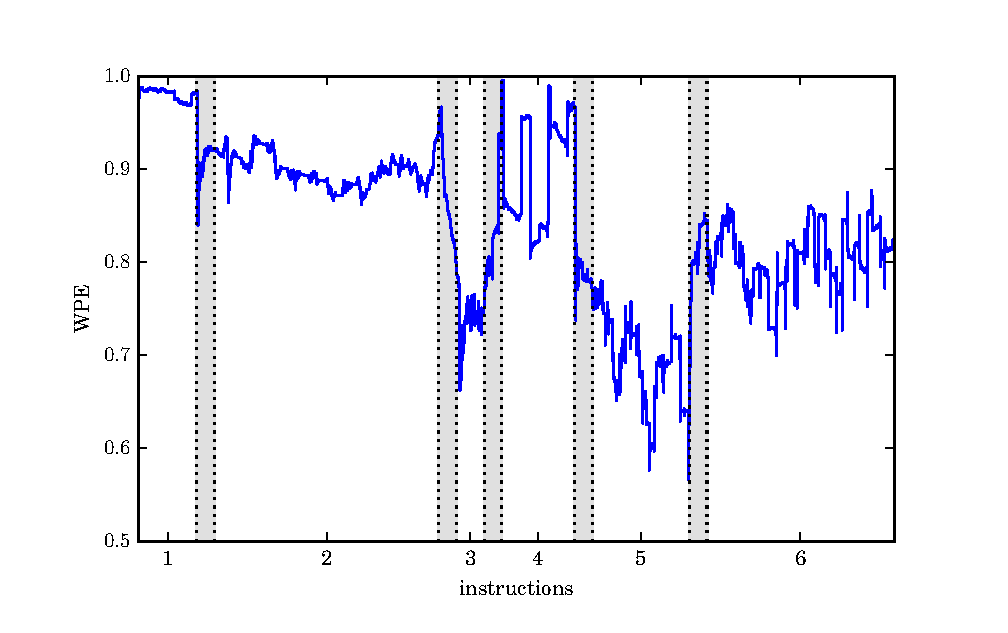
\includegraphics[width=1.0\textwidth]{figs/SVD_wwpe}
%  \caption{[[Joshua: I think adding the colored SVD trace to this would be %good or putting it above this figure]]The weighted permutation entropy of %one run of SVD. The gray bands
%    are regions where the window overlaps regimes. The window size used is
%    $5,000 \times 100,000$ instructions and the word length is $4$.}
%  \label{fig:wwpe}
%\end{figure}


%%FIGURE INTENT
%This figure shows that entropy changs over time with the signal as well as why the regimes for \svd were chosen. 
%%%%%%%%%%%%%%%%%
\begin{figure}[htbp]
  \centering
  %\begin{subfigure}{0.3\textwidth}
  %  \includegraphics[width=0.3\textwidth]{figs/svdipcregimescolored.png}
  %  \caption{The instructions per cycle of \svd. Each color corresonds to the different regimes as selected by rapid shifts in WPE, as seen in Figure \ref{fig:svd_wwpe}. From left to right each change in color represents a change in regime for 6 regimes in total. }
 %   \label{fig:svd_ts}
 % \end{subfigure}%
  %\\
 % \begin{subfigure}{\textwidth}

%Liz commented this image out temporarily so that her mac doesn't hang
%when she scrolls past p12
    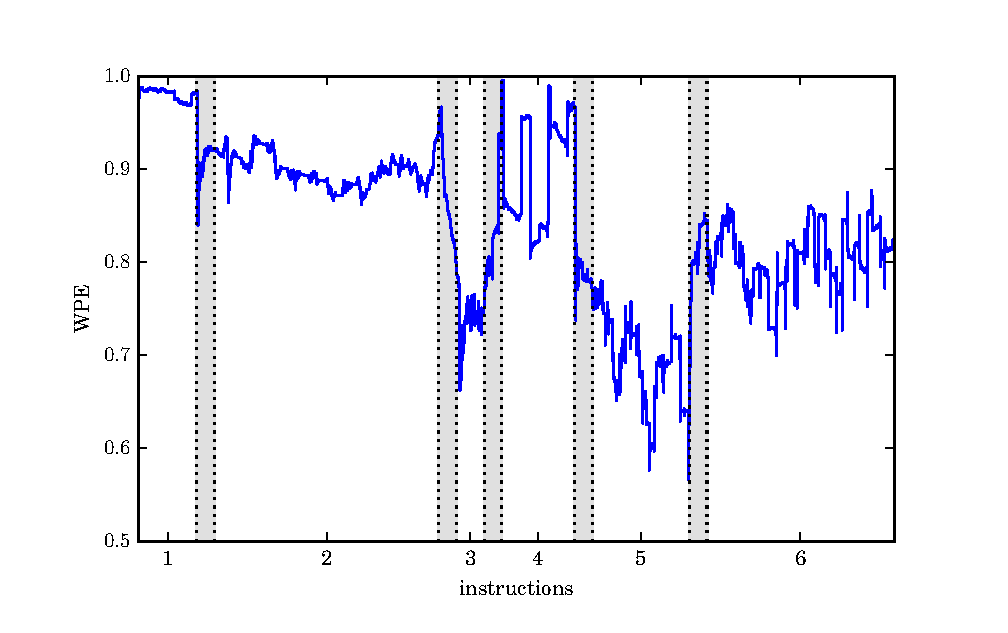
\includegraphics[width=\columnwidth]{figs/SVD_wwpe}
    %\caption{The MASE of ARIMA vs weighted permutation entropy. }
  \caption{The weighted permutation entropy of one run of
  SVD. The gray bands are regions where the window overlaps
  regimes. The window size used is 5,000 $\times$ 100,000 instructions
  and the word length is $6$. {\color{red} make sure this is actually updated to 6} For reference the instructions per cycle
  of \svd are plotted as a ghost behind this plot. Each color on the
  ghosted time series corresonds to the different regimes as selected
  by rapid shifts in WPE. From left to right each change in color
  represents a change in regime for 6 regimes in
  total.}\label{fig:wwpe}
\end{figure}







 \section{Validation of Primary Findings} % (fold)
 \label{sec:results}


%OUTLINE:
%\begin{enumerate}
%\item \cmark~Introduce MASE.
%\item \cmark~WPE is a good measure of predictability.  %Figure: best athlete MASE vs.
%its WPE.
%\item \cmark~Talk about structure analysis. Just because %there is forward information
%transfer, does not mean that linear predictors can get at %this.
%\subitem \cmark~For this show a figure of (a) ARIMA vs MASE %(b) LMA vs MASE in a side by%
%side plot.
%\item full results.  Image: MASE vs. WPE for both LMA \& %ARIMA.  Points to make:
%\begin{enumerate}
%\item \cmark~clusters are distributed differently
%\item \cmark~clusters are shaped differently---tight or not
%\item \cmark~clusters move differently between LMA and ARIMA
%\item finally, the diagonal line is important. If you're %below it, you could do
%better.
%\end{enumerate}
%\end{enumerate}

%BRAINSTORMING 
%\begin{itemize}
%\cmark\item The kind of complexity present matters, i.e., that is whether the complexity is structured or not.[[use here and mention in intro]] 
%\cmark\item Quantifying structured and unstructured complexity is nontrivial in the case of real-valued noisy time series but WPE does this. [[talk about again here but justify in information theory section]]
%\item Maybe plot a big chunk of \col and a big chunk of \gcc together and show that they both look complex. 

%\cmark\item \gcc appears visually very complex, *and* according to WPE this complexity is unstructured. And a constant, linear and nonlinear prediction strategy all fail. We should be able to conclude that guessing random values is the best we can do as is shown by MASE [[Use in this section]]

%\cmark\item \col is also complex (can even be chaotic/ point to CHAOS paper) but the complexity is structured according to WPE and as such that complexity is usable for prediction [[use in this section]]

%\cmark\item \col brings about the point nicely that some prediction strategies cannot utilize the processes internal information transfer method. That is a nonlinear internal information transfer system cannot be predicted effectively with a linear strategy. This gives a practitioner leverage on when to give up and when to keep working. [[use in this section as bridge to next section]]

%\end{itemize}


In this section we validate the two key primary findings of this work which we introduced in Section \ref{sec:intro}:



\begin{enumerate}

\item The existence of predictable structure in noisy real-valued time series is quantifiable by WPE and as a result WPE is correlated with prediction accuracy (MASE) of an ideal predictor. 

%\subitem [[Simply reminders not to be included]]WPE can quantify when a noisy real-valued time series is predictable.[[I am unsatisfied with predictable in this sentence, need a better word to say "better than random walk" or ``able to be forecast effectively" or ``has the structural capacity to transmit information in a way that the time series can be effectively forecast"

%\item The existence of complex structure in a noisy real-valued time series is quantifiable and this type of complexity is directly correlated with predictability

\item The way structure/information/complexity is processed internally by a given process plays a crucial role in predictability.


%\subitem [[Simply reminders not to be included]]We will have shown that the existence whether linear or nonlinear is picked up on with WPE but this point gets at whether the prediction model can use the structure or not (linear can't use nonlinear structure). The right to left shifts in \col and some of the \svd regimes and the lack of shift in \gcc illustrate this nicely.

%\subitem [[Simply reminders not to be included]]This is the linear vs nonliear vs random we see with the right to left shifts with lower complexity time series. 

\end{enumerate}



%This portion should justify the following claim%%%%%%%%%%%%%%%%%%%%%%
%\item The existence of predictable structure in noisy real-valued time series is quantifiable by WPE and as a result WPE is correlated with prediction accuracy (MASE)  
%%%%%%%%%%%%%%%%%%%%%%%%%





%\item First paragraph: WPE is a good measure of predictability.  Figure:
%best athlete MASE vs. its WPE. 


%\item Quantifying structured and unstructured complexity is nontrivial in the case of real-valued noisy time series but WPE does this. [[talk about again here but justify in information theory section]]

As we discussed in Section \ref{sec:meaComplex} distinguishing structured from unstructured complexity in the case of real-valued time series is non trivial, i.e., distinguishing when a complex signal omits predictable structure and when the signal is effectively random is not a trivial task. As described in Section \ref{sec:intro}, for a practitioner this can be frustrating because it can be nearly impossible to find the source of faulty predictions: Is it simply that we need to use a more ideal (possibly more advanced) predictor or is it the case that the time series is simply so complex that using a simple (yet inconsistent) forecast strategy such as random walk is the best we can do. Fortunately, weighted permutation entropy (WPE) allows us to make this distinction for noisy real-valued time series. 

In Figure~\ref{fig:pred_vs_wpe} we plot the best prediction (i.e., the lowest MASE over all 3 methods\footnote{LMA,ARIMA,na\"ive} over all 15 runs of that program) for each of the 8 programs under investigation. 
\begin{figure}[htbp]
  \centering
  \includegraphics[width=0.75\textwidth]{figs/prediction_vs_entropy}
  \caption{The best MASE among all runs and prediction methods vs weighted
  permutation entropy. For each of these, the word length used is $6$. The
  dashed line is a least-squares linear fit of all the points except for {\tt
  SVD$_1$} which we have excluded for reasons explained in the text.}
  \label{fig:pred_vs_wpe}
\end{figure}
What we see here is that the relationship between prediction accuracy (MASE) and the weighted permutation entropy is much as we conjectured: The existence of predictable structure in noisy real-valued time series as quantified by low to moderate WPE  is correlated with prediction accuracy (MASE) of the ``best"predictor\footnote{We do not claim to have found the ideal predictor for each signal, simply the best predictor over what we used; Which we believe to be a fair sampling of standard prediction techniques for this type of signal.}. We will not further validate this claim through some examples. 


To further validate this finding we present an in-depth analysis of three examples (\col, \svdfive and \gcc ) which nicely cover the range of complexity from low to high respectively. In Figures~\ref{fig:lma_vs_arima} and \ref{fig:arima_pred_vs_ent} we plot the MASE of LMA and ARIMA (respectively) against the weighted permutation entropy of each of the 15 runs of all 8 programs. We also list all of these values in Table \ref{tab:error}

\begin{table}[htdp]
\caption{MASE distributions for 1-step predictions at a 10\% prediction horizon over 15 runs for each signal and average wpe at word length 6 for each signal.}
\begin{center}
\begin{tabular}{|c|c|c|c|c|}
\hline
                   & MASE LMA    & MASE ARIMA &MASE na\"{i}ve   & $l=6$ \\
\hline
\gcc                  & $ 1.5296\pm 0.0214$ & $1.8366 \pm0.0157 $ & $0.9510 \pm 0.0011$ & $0.9430 \pm 0.0013$ \\

\col           & $ 0.0500 \pm0.0018  $ & $0.5989  \pm 0.2114 $ & $0.5707\pm0.0017$&  $0.5131 \pm 0.0034$ \\

\svd Reg. 1     & $ 0.8273\pm 0.0755$ & $ 0.7141\pm 0.0745 $ & $2.6763\pm4.3282$&  $0.9572 \pm 0.0156$ \\
\svd Reg. 2     & $1.2789 \pm0.0196 $ & $2.1626 \pm0.0265 $ &  $3.0543\pm0.0404$ &   $0.8464 \pm0.0044$ \\
\svd Reg. 3       & $0.6192 \pm0.0209 $ & $0.7129 \pm 0.0096 $ & $31.3857\pm 0.2820$ &  $0.7157 \pm 0.0056$ \\
\svd Reg. 4     & $ 0.7789\pm0.0358 $ & $0.9787 \pm0.0321 $ & $2.6613\pm0.0739$ & $0.8246 \pm 0.0077$ \\
\svd Reg. 5     & $ 0.7177\pm 0.0483 $ & $2.3700  \pm 0.0505 $ & $20.8703 \pm 0.1915$&  $0.6776 \pm 0.0068$ \\
\svd Reg. 6     & $ 0.7393\pm 0.0682 $ & $ 1.4379\pm 0.0609$ & $2.1967\pm0.0830$&  $0.7475 \pm 0.0106$ \\
\hline
\end{tabular}
\end{center}
\label{tab:error}
\end{table}%





\begin{figure}[htbp]
  \centering
       
  \begin{subfigure}{0.5\textwidth}
    \includegraphics[width=\textwidth]{figs/LMA_prediction_vs_entropy}
    \caption{The MASE of LMA vs weighted permutation entropy. }
    \label{fig:lma_pred_vs_ent}
  \end{subfigure}%
  \begin{subfigure}{0.5\textwidth}
    \includegraphics[width=\textwidth]{figs/ARIMA_prediction_vs_entropy}
    \caption{The MASE of ARIMA vs weighted permutation entropy. }
    \label{fig:arima_pred_vs_ent}
  \end{subfigure}
\caption{
For each of these, the word length used is $6$. The MASE values for LMA against ARIMA. The dashed line is the identity, delineating the traces for which either LMA or ARIMA performed better. All traces except those from \svd$_1$ lie above the line, indicating that LMA is better suited prediction method for the computer traces considered.}\label{fig:lma_vs_arima}  
\end{figure} 

We will start with the lowest complexity program: \col. Conceptually this program is very simple but due to computer design choices this program can result in highly complex even chaotic time series traces, see \cite{mytkowicz09}. If we forecast this signal using an out-of-the-box linear forecaster (ARIMA) or an out-of-the-box constant predictor we receive MASE ($0.59 \pm 0.21$ and $0.57 \pm$ 0.001 respectively) which suggest that on average we can only predict this signal twice as well as the simple random walk prediction. This would suggest that there is some predictive structure present but not that much. However, if we quantify the predictive structure present in this signal using WPE we see that this signal is highly structured with a WPE of ($0.51 \pm 0.003$.) The existence of structured which we quantified with WPE implies that an ideal predictor capable of using this signals information should be able to predict this signal much better than the random walk due to the high amount of predictive structure or equivalently the low complexity. This is in fact the case. \col is a complex signal, i.e., chaotic, but it is complex in a structured way. Using a prediction technique that can process nonlinear information yields forecasts with a MASE of $0.05 \pm 0.001$, this is a prediction 20 times more accurate than a random walk forecast. The existence of predictive structure as quantified by WPE could be precisely the information needed to continue searching for an ideal predictor like LMA. 

Maybe even more convincing than a low complexity signal like \col is a moderately complex signal like \svdfive. This signal omits a WPE of $0.677 \pm 0.006$, this is a significantly higher complexity than \col but still implies the existence of a great deal of predictive structure. However, this increase in complexity is enough to really throw off the constant and linear prediction strategies. The MASE scores for ARIMA and na\"ive imply 2.5 and 20 times worse prediction than using a simple random walk forecast. This may be discouraging to someone using an out-of-the-box predictor that the signal is too complex to predict. However by \emph{knowing} that there exists predictable  in this signal we can try to use a more advanced technique, in particular LMA. If we do this we get forecasts which score 1.5 times better than the random walk. Showing that this usable structure (although hidden to the linear and constant method) was quantifiable by WPE.

Finally, we consider the most complex program: \gcc. The complexity of \gcc is $0.94 \pm 0.001$. This implies that almost no predictive structure exists in this structure. Recall that a WPE $\approx 1$ are similar in complexity to white noise or a random walk process as they do not transmit any information from past to future. This would mean that the WPE of $>0.95$ would suggest little to no predictive structure exists and that the signal is simply too complex. In this case it should be safe to assume that a random walk forecast would be (on-average) superior to forecast methods which required structure or information to intelligently predict the next time step. This is in fact what we see, with each prediction scheme we used we see a MASE which implies (on-average) 1.5-1.8 times worse predictions that performing a simple random walk forecast. 

There is a single outlier in this study which is \svdone. This signal has a WPE of $0.95 \pm 0.02$ and both LMA and ARIMA do slightly better than random walk ($0.82 \pm 0.08$ and $0.7141 \pm 0.07$ respectively). The na\"ive method did significantly worse than random walk and was highly inconsistent with an average MASE of 2.67 but a standard deviation of 4.33 due to the massive right tail this distribution exhibited in reaction to wildly inconsistent forecasts. We do not believe this outlier is really a problem but it does bring about a potential weaknesses of this method. MASE is scaled by a random walk forecast which can be very inconsistent in the case of drastic signal changes which occur on a regular basis, e.g., a signal which oscillates from the top to the bottom of the signals scale at every time click. In this case a random walk forecast would have error with magnitude of the scale of the signal at every forecast, since guessing the last step will be exactly out of phase with the new forecast. A signal like this would normally cause a very low WPE much like \col and a very high Random Walk error resulting in low MASE for methods that can take into account this structure like ARIMA or LMA. 

To understand why this causes \svdone to be an outlier we examine Figure \ref{fig:svdone-ts} in more detail. This is a small snippet of the time series of \svdone to illustrate the strucutre of this signal. We provide a small snippet as opposed to the full time series simply for visual clarity.
\begin{figure}[htbp]
  \centering
    \includegraphics[width=\textwidth]{figs/svdonets2}
\caption{ For each of these, the word length used is $6$. The MASE values for LMA against ARIMA. The dashed line is the identity, delineating the traces for which either LMA or ARIMA performed better. All traces except those from \svd$_1$ lie above the line, indicating that LMA is better suited prediction method for the computer traces considered.}\label{fig:svdone-ts}  
\end{figure} 
As can be seen in Figure \ref{fig:svdone-ts}, \svdone has a highly unstructured small band on top, which is approximately 0.05 instructions per cycle wide. Approximately 80\% of the signal exists within this band of noise, this causes the WPE to be driven up as many words are being omitted by this band of the signal. The remaining 20\% of the signal are drops in instructions per cycle away from this band, ranging in size from 0.1 to 0.6 instructions per cycle\footnote{Some of the large drops are not shown for the sake of clarity of the smaller scale}. These drastic drops seem to happen every 5-7 points but the drop locations are inconsistent as well as the drops magnitude (ranging from 0.1-0.6 instructions per cycle). As discussed in Section \ref{sec:RWMethod} drops of this fashion are the bane of random walk forecasting. At every one of these drops a random walk predictor would produce two forecasts with an error 2-12 times the magnitude of the smaller band, i.e., about 40\% of the time the random walk forecast would predict with error 2-12 times the magnitude of the scale exhibited by $\approx$80\% of the signal. This inconsistency in random walk would cause cause random walk error to be high and as a result MASE scores to be artificially low. The combination of a band of noise with a high number of random drops is a weakness of this method which is present in \svdone and as a result makes this signal an outlier.


[[Joshua: I am not sure if this paragraph is strong enough or even worth having]]These results support that time series with low to moderate complexity ($0\le WPE \le 0.85$) can be predicted more efficiently than a na\"ive random walk \emph{and} that complexity can be qualitatively measured for a real-valued noisy time series using WPE. This will allow practitioners to stop spinning their wheels in the case of signals who are simply better predicted with a simple strategy like random walk. The analysis of these results illuminates an interesting point: The way structure, information and complexity are processed by a generating process plays a crucial role in the success of a given prediction scheme. 











%This portion should justify the following claim%%%%%%%%%%%%%%%%%%%%%%
%\item The way structure/information/complexity is processed internally by a given process plays a crucial role in predictability.
%%%%%%%%%%%%%%%%%%%%%%%%%






Comparing Figures~\ref{fig:lma_pred_vs_ent} and \ref{fig:arima_pred_vs_ent} also elucidates another key finding: usable and quantifiable predictive structure can be present in a time series without a prediction scheme being able to utilize it. In particular, information may be transferred from past to future through the present but because of the mechanism the underlying process uses to process that information  (e.g., linear or nonlinear) certain prediction strategies may be blind to or not be able to efficiently utilize this information. For example, consider \col, programs like this have been shown to exhibit deterministic chaos \cite{mytkowicz09}. If this were the case with \col, an out-of-the-box linear method like ARIMA would simply be ill-equipped to model and utilize the kind of structure present, as is evident in Figure \ref{fig:arima_pred_vs_ent}. In contrast, a nonlinear predictor like LMA which is built to handle deterministic chaos, can interpret and utilize this type of structure just fine. We believe that many of the shifts in forecast accuracy for low-to-moderate WPE programs between ARIMA and LMA is precisely happening for this reason: Just because there is forward information transfer, does not mean that an arbitrary predictor can interpret or utilize it, but luckily WPE can tell us when this structure is present as shown in Figure \ref{fig:lma_vs_arima}.

%In Figures~\ref{fig:lma_pred_vs_ent} and \ref{fig:arima_pred_vs_ent} we directly compare the performance of the LMA and ARIMA prediction methods (respectively) to the value of the weighted permutation entropy for all runs of each program under consideration. The LMA MASE values are largely similar to those of the best predictions, primarily because LMA often performed superior to ARIMA (and the na\"ive method). On the other hand, the ARIMA MASE values are largely uncorrelated with WPE values. As was hinted at while discussing the previous results, the fact that ARIMA is uncorrelated with WPE brings about an interesting perspective on information transfer and WPE. The WPE is sensitive to both linear and nonlinear structure. When you have a low WPE and a high ARIMA it could be that the structure WPE is picking up is simply nonlinear structure that LMA can handle but ARIMA cannot. So while ARIMA is consistently out performed by random walk,  there is plenty of structure present as suggested by WPE and taken advantage of by LMA but since it is nonlinear ARIMA can't take it into account and does bad.



%is in large part one of the major findings of this work. More specifically, say we tried to predict an arbitrary noisy real-valued time series with an ``out-of-the-box" prediction strategy like ARIMA as proposed in \cite{autoArima} and say we got inconsistent and bad forecasts, (i.e., perform worse than the na\"ive random walk strategy (MASE$>1$). How do we determine if the prediction strategy is not adequate for the prediction task, or if the signal is simply too complex to predict. If a signal is too complex and too little forward information transfer is present we may not be able to do better than the random walk, in which case we should not worry ourselves over finding a more complicated prediction strategy. However, if we measure the complexity to be low, $\textrm{WPE}<0.85$ (see Fig.~\ref{fig:pred_vs_wpe}) we can most likely do much better than the random walk and should search for more adequate prediction strategies. 




 


Other noteworthy features of the LMA and ARIMA results are the cluster locations
and distributions. The WPE values of each run of any particular program tend to
have little variance, leading to the clusters in
Figures~\ref{fig:arima_pred_vs_ent} and \ref{fig:lma_pred_vs_ent} to be fairly
constrained in the $y$ direction. For most traces, the LMA and ARIMA variance is
low as well, resulting is small, tight clusters. The ARIMA MASE values of the \col
traces, however, have a large variance resulting in the spread seen in
Figure~\ref{fig:arima_pred_vs_ent}. Not only are the MASE values of that cluster
bad, in that other predictors vastly outperform it, but they are inconsistent.
Furthermore, since LMA can predict nonlinear behavior while ARIMA cannot, we
see that the clusters in Figure ~\ref{fig:arima_pred_vs_ent} are mostly further to
the right than those in Figure~\ref{fig:lma_pred_vs_ent}.



\section{ Conclusions \& Future Work }\label{sec:conc}

Forecast strategies that are designed to capture predictive structure
are ineffective when signal complexity outweighs information
redundancy.  This poses a number of serious challenges in practice.
First, without knowing anything about the generating process, it is
difficult to determine how much predictive structure is present in a
given time series.  And even if predictive structure exists, a given
forecast method may not work, simply because it cannot exploit the
structure that is present (e.g., a linear model of a nonlinear
process).  If a forecast model is not producing good results, a
practitioner needs to know why: is the reason that the time series
contains no predictive structure---i.e., that no model will work---or
is the model that s/he is using simply not good enough?

In this paper, we have argued that redundancy~\cite{crutchfield2003}
is a useful definition of the inherent predictability of a time
series.  To operationalize that definition, we use an approximation of
the Kolmogorov-Sinai entropy~\cite{lind95}, estimated using a weighted
version of the permutation entropy of~\cite{bandt2002per}.  This WPE
technique---an ordinal calculation of forward information transfer in
a time series---is ideal for our purposes because it works with
real-valued data and is known to converge to the true entropy value.
Using a variety of forecast models and more than a hundred time-series
data sets from a computer-performance experiment, we have shown that
prediction accuracy is indeed correlated with weighted permutation
entropy: the higher the WPE, in general, the higher the prediction
error.  There are some exceptions: [[Liz to do: summarize \& discuss
    here.]]

% Further, the persistent WPE values of 0.5--0.6 for the {\tt
%   col\_major} trace are consistent with dynamical chaos, further
% corroborating the results of~\cite{mytkowicz09}.

An important practical corollary to this empirical correlation of
predictability and WPE is a practical strategy for assessing
appropriateness of forecast methods.  If the forecast produced by a
particular method is poor but the time series contains a significant
amount of predictive structure, one can reasonably conclude that that
method is inadequate to the task and that one should seek another
method.  The nonlinear LMA method, for instance, performs better in
most cases because it is more general.  The \naive ~method, which
simply predicts the mean, works better in noisy signals because it
effects a filtering operation.  The simple random-walk strategy is
better than LMA, ARIMA, or the \naive ~method on the \gcc signal,
which is extremely complex---i.e., extremely low redundancy.
{\color{red} I suggest we don't mention \svdone here since it's a
  pretty detailed thing and conclusions are for high-level summaries.
  It's a good point, though, and I'll leave it in comments in the
  file.}
%  \naive ~wins on \svdone with the exception to the 5 outliers.
The dashed line in Figures~\ref{fig:wpe_vs_mase_best}
and~\ref{fig:wpe_vs_mase_all} is a useful empirical guideline for
knowing when a model is not well-matched to the task at hand: a $MASE$
score that is more than {\color{red}[[what's the equation for that
      line, Ryan?]]} times the WPE of the corresponding signal is an
indication that that time series has more predictive structure than
that forecast model can capture and exploit.

Given that information is a fundamental limitation in predictability,
then gathering and using more information is an obvious next step.
But there is an equally obvious tension here between data length and
prediction speed: a forecast that requires half a second to compute is
not useful for the purposes of real-time control of a computer system
with a MHz clock rate.  Another alternative is to sample several
system variables simultaneously and build multivariate models.  This
is a particular challenge in nonlinear LMA-type models, since
multivariate delay-coordinate embedding (e.g.,
\cite{cao-multivariate-embedding,deyle-sugihara2011}) can be
computationally prohibitive.  We are working on alternative methods
that sidestep that complexity.

%Paragraphs on the issues that come up, including one about the "amount
%of info" one: if one could sample more variables, for instance, one
%might be able to do a better job of predicting more-complex traces.
%Segue to some handwaving about multivariable LMA models; tie this back
%to the "computers are NLD systems" stuff in the intro.  This is a real
%challenge; current approaches to this modelling problem have the major
%issue of taking way too long to build.  And that's a big issue if
%you're trying not just to classify, but to predict.  In a system that
%runs at MHz speeds, a prediction that takes milliseconds to compute is
%not useful.
%\end{it}

Nonstationarity is a serious challenge in any time-series modeling
problem.  Indeed, one of the first applications of permutation entropy
was regime-shift detection for the purposes of recognizing seizure
onset in brainwave data~\cite{cao2004det}.  Recall that the signal in
Figure~\ref{fig:svd-ts-colored} was especially useful for the study in
this paper because it contained a number of different regimes.  We
segmented this signal visually, but one could imagine using
permutation entropy to do so instead.  Automating regime-shift
detection would be an important step towards a fully adaptive modeling
strategy, where old models are discarded and new ones are rebuilt
whenever shifts are detected.  WPE would be particularly powerful in
this scenario, as its value can suggest what kind of model might work
well in each new regime.

All of the experiments described in this paper involve a particular
physical system.  We chose that system because its behavior spans a
broad spectrum of classical time series patterns.  We believe that our
results will generalize far beyond this particular system; proving
that claim with examples is another important next step.  [[Liz to do:
    insert some examples.  Close with mention of what that could
    enable (viz., adaptive models like ones at end of prev paragraph
    used as the core of controllers).]]

% The way structure, information and complexity are processed by a
% generating process play a crucial role in the success of a given
% prediction scheme.




\section*{Acknowledgment}
This work was partially supported by NSF grant \#CMMI-1245947 and ARO
grant \#W911NF-12-1-0288.

\section{Appendix}

\begin{table}[h]
  \begin{center}
  \begin{tabular}{|c|c|c|c|c|}
  \hline
            & MASE LMA    & MASE ARIMA &MASE na\"{i}ve   & $l=6$ \\
 \hline 
 
 \col           & $ 0.050 \pm0.002  $ & $0.599  \pm 0.211 $ & $0.571\pm0.002$&  $0.513 \pm 0.003$ \\

\gcc           & $ 1.530\pm 0.021$ & $1.837 \pm0.016 $ & $0.951 \pm 0.001$ & $0.943 \pm 0.001$ \\

\svdone     & $ 0.827\pm 0.076$ & $ 0.714\pm 0.075 $ & $2.676\pm4.328$&  $0.957 \pm 0.016$ \\

 \svdtwo    & $1.279 \pm0.020 $ & $2.163 \pm0.027 $ &  $3.054\pm0.040$ &   $0.846 \pm0.004$ \\
 
 \svdthree     & $0.619 \pm0.021 $ & $0.713 \pm 0.010 $ & $31.386\pm 0.282$ &  $0.716 \pm 0.006$ \\

 \svdfour     & $ 0.779\pm0.036 $ & $0.979 \pm0.032 $ & $2.661\pm0.074$ & $0.825 \pm 0.008$ \\
 
 \svdfive     & $ 0.718\pm 0.048 $ & $2.370  \pm 0.051 $ & $20.870 \pm 0.192$&  $0.678 \pm 0.007$ \\
 
 \svdsix     & $ 0.739\pm 0.068 $ & $ 1.438\pm 0.0610$ & $2.197\pm0.083$&  $0.748 \pm 0.011$ \\
  \hline
  \end{tabular}
  \end{center}
 \label{default}
 \caption{Detailed MASE scores}
 \label{tab:error}
  \end{table}%




\bibliographystyle{aipauth4-1}
\bibliography{bibliofile}


\end{document}
